%!TEX root = ../THESIS.tex

\usepackage[utf8]{inputenc}
\usepackage[english]{babel}
\usepackage{textgreek}

\usepackage{breakurl}
\usepackage{hyperref}

\usepackage[
    style=alphabetic,
    sorting=nyt,
    backend=biber,
    maxbibnames=99,
    doi=true,
    isbn=false,
    url=true
]{biblatex}
\renewcommand*{\bibfont}{\raggedright\small}

% https://tex.stackexchange.com/questions/154864/biblatex-use-doi-only-if-there-is-no-url/154875#154875
\DeclareSourcemap{
  \maps[datatype=bibtex]{
    \map{
      \step[fieldsource=doi,final]
      \step[fieldset=url,null]
      \step[fieldset=urldate,null]
    }
    \map{
      \step[fieldsource=eprint,final]
      \step[fieldset=url,null]
      \step[fieldset=urldate,null]
    }
  }
}

% https://tex.stackexchange.com/questions/163774/biblatex-print-bibliography-for-a-single-entry-within-an-enumeration
\DeclareBibliographyCategory{enumpapers}

\newcommand{\enumcite}[1]{%
  \nocite{#1}
  \addtocategory{enumpapers}{#1}%
  \defbibcheck{key#1}{
    \iffieldequalstr{entrykey}{#1}
      {}
      {\skipentry}}%
  \printbibliography[heading=none,check=key#1]%
}

\usepackage{amsthm, amssymb, amsmath}

\usepackage{setspace}
\renewcommand{\baselinestretch}{1.25}

\usepackage[frozencache]{minted}
\usemintedstyle{lovelace}
\setminted{frame=lines,fontseries=mono,fontsize=\footnotesize}
\setmintedinline{fontsize=auto}
\BeforeBeginEnvironment{minted}{\vspace{-16pt}}
\AfterEndEnvironment{minted}{\vspace{-8pt}}

\newcommand{\py}[1]{{\color{brown}\mintinline{python}{#1}}}

\newcommand{\inputpython}[1]{
{\vspace{-10pt} \footnotesize \inputminted[baselinestretch=1]{python}{#1}} \vspace{-10pt}}

\usepackage{caption}
\usepackage{subcaption}

\usepackage{graphicx}
\graphicspath{ {./img/} }

\usepackage{tikz}
\usepackage{tikz-cd}
\usepackage{src/tikzit}
\input{src/qcs.tikzstyles}

\usepackage[perpage]{footmisc}

\usepackage{ragged2e}
\usepackage{epigraph}
\setlength{\epigraphwidth}{0.55\textwidth}
\newcommand{\justepigraph}[2]{
\epigraph{\footnotesize \justifying #1}{#2}}


%!TEX root = ../THESIS.tex

\newcommand{\xto}[1]{\xrightarrow{#1}}
\newcommand{\sub}{\subseteq}
\newcommand{\s}{\enspace}
\newcommand{\eval}[1]{[ \! [ #1 ] \! ]}

\newcommand{\bra}[1]{\langle#1|}
\newcommand{\ket}[1]{|#1\rangle}
\newcommand{\braket}[2]{\langle#1|#2\rangle}

\newcommand{\dom}{\mathtt{dom}}
\newcommand{\cod}{\mathtt{cod}}
\newcommand{\id}{\mathtt{id}}
\newcommand{\then}{\mathtt{then}}
\newcommand{\tensor}{\mathtt{tensor}}
\newcommand{\len}{\mathtt{len}}

\renewcommand{\S}{\mathbb{S}}
\newcommand{\B}{\mathbb{B}}
\newcommand{\N}{\mathbb{N}}
\newcommand{\Z}{\mathbb{Z}}
\newcommand{\R}{\mathbb{R}}
\renewcommand{\C}{\mathbb{C}}

\def\fcmp{\mathbin{\raise 0.6ex\hbox{\oalign{\hfil$\scriptscriptstyle      \mathrm{o}$\hfil\cr\hfil$\scriptscriptstyle\mathrm{9}$\hfil}}}}


\newcommand{\downmapsto}{\rotatebox[origin=c]{-90}{$\mapsto$}\mkern2mu}


\newtheorem{definition}{Definition}[section]
\newtheorem{proposition}[definition]{Proposition}
\newtheorem{theorem}[definition]{Theorem}
\newtheorem{conjecture}[definition]{Conjecture}
\newtheorem{lemma}[definition]{Lemma}
\newtheorem{corollary}[definition]{Corollary}
\newtheorem{example}[definition]{Example}
\newtheorem{remark}[definition]{Remark}
\newtheorem{python}[definition]{Listing}


\title{Category Theory for Quantum\\
Natural Language Processing}
\author{Alexis TOUMI}
\college{Wolfson College}

\degree{Doctor of Philosophy}
\degreedate{\today}

\addbibresource{THESIS.bib}

\begin{document}
\begin{romanpages}
\maketitle

This thesis introduces quantum natural language processing (QNLP) models based on a simple yet powerful analogy between computational linguistics and quantum mechanics: grammar as entanglement.
The grammatical structure of text and sentences connects the meaning of words in the same way that entanglement structure connects the states of quantum systems.
Category theory allows to make this language-to-qubit analogy formal: it is a monoidal functor from grammar to vector spaces.
We turn this abstract analogy into a concrete algorithm that translates the grammatical structure onto the architecture of parameterised quantum circuits.
We then use a hybrid classical-quantum algorithm to train the model so that evaluating the circuits computes the meaning of sentences in data-driven tasks.

The implementation of QNLP models motivated the development of DisCoPy (Distributional Compositional Python), the toolkit for applied category theory of which the first chapter gives a comprehensive overview.
String diagrams are the core data structure of DisCoPy, they allow to reason about computation at a high level of abstraction.
We show how they can encode both grammatical structures and quantum circuits, but also logical formulae, neural networks or arbitrary Python code.
Monoidal functors allow to translate these abstract diagrams into concrete computation, interfacing with optimised task-specific libraries.

The second chapter uses DisCopy to implement QNLP models as parameterised functors from grammar to quantum circuits.
It gives a first proof-of-concept for the more general concept of functorial learning: generalising machine learning from functions to functors by learning from diagram-like data.
In order to learn optimal functor parameters via gradient descent, we introduce the notion of diagrammatic differentiation: a graphical calculus for computing the gradients of parameterised diagrams.


% \flushbottom
\tableofcontents

% The Roman pages, like the Roman Empire, must come to its inevitable close.
\end{romanpages}

\chapter*{Introduction}
\addcontentsline{toc}{chapter}{Introduction}
\markboth{Introduction}{Introduction}

%!TEX root = ../THESIS.tex

\section*{What are quantum computers good for?}
\addcontentsline{toc}{section}{What are quantum computers good for?}

\justepigraph{
Nature isn't classical, dammit, and if you want to make a simulation of nature, you'd better make it quantum mechanical, and by golly it's a wonderful problem, because it doesn't look so easy.
}{\textit{Simulating Physics with Computers}, Feynman (1981)}

Quantum computers harness the principles of quantum theory such as superposition and entanglement to solve information-processing tasks.
In the last 42 years, quantum computing has gone from theoretical speculations to the implementation of machines that can solve problems beyond what is possible with classical means.
This section will sketch a brief and biased history of the field and of its future challenges.

In 1980, Benioff~\cite{Benioff80} takes the abstract definition of a computer and makes it physical: he designs a quantum mechanical system whose time evolution encodes the computation steps of a given Turing machine.
In retrospect, this may be taken as the first proof that quantum mechanics can simulate classical computers.
The same year, Manin~\cite{Manin80} looks at the opposite direction: he argues that it would take exponential time for a classical computer to simulate a generic quantum system.
Feynman~\cite{Feynman82,Feynman85} comes to the same conclusion and suggests a way to simulate quantum mechanics much more efficiently: building a quantum computer!

So what are quantum computers good for? Feynman's intuition gives us a first, trivial answer: at least quantum computers could simulate quantum mechanics efficiently. Deutsch~\cite{Deutsch85a} makes the question formal by defining quantum Turing machines and the circuit model.
Deutsch and Jozsa~\cite{DeutschJozsa92} design the first quantum algorithm and prove that it solves \emph{some} problem exponentially faster than any classical \emph{deterministic} algorithm.\footnote
{A classical \emph{randomised} algorithm solves the problem in constant time with high probability.}
Simon~\cite{Simon94} improves on their result by designing a problem that a quantum computer can solve exponentially faster than any classical algorithm.
Deutsch-Jozsa and Simon relied on oracles\footnote{An oracle is a black box that allows a Turing machine to solve a certain problem in one step.}
and promises\footnote{The input is promised to satisfy a certain property, which may be hard to check.} and their problems have little practical use.
However, they inspired Shor's algorithm~\cite{Shor94} for prime factorisation and discrete logarithm. These two problems are believed to require exponential time for a classical computer and their hardness is at the basis of the public-key cryptography schemes currently used on the internet.

In 1997, Grover provides another application for quantum computers: ``searching for a needle in a haystack''~\cite{Grover97}.
Formally, given a function $f : X \to \{0, 1\}$ and the promise that there is a unique $x \in X$ with $f(x) = 1$, Grover's algorithm finds $x$ in $O(\sqrt{|X|})$ steps, quadratically faster than the optimal $O(|X|)$ classical algorithm.
Grover's algorithm may be used to brute-force symmetric cryptographic keys twice bigger than what is possible classically~\cite{BernsteinEtAl09}.
It can also be used to obtain quadratic speedups for the exhaustive search involved in the solution of NP-hard problems such as constraint satisfaction~\cite{Ambainis04}.
Independently, Benett et al.~\cite{BennettEtAl97} prove that Grover's algorithm is in fact optimal, adding evidence to the conjecture that quantum computers cannot solve these NP-hard problems in polynomial time.
Chuang et al.~\cite{ChuangEtAl98} give the first experimental demonstration of a quantum algorithm, running Grover's algorithm on two qubits.

Shor's and Grover's discovery of the first real-world applications sparked a considerable interest in quantum computing.
The core of these two algorithms has then been abstracted away in terms of two
subroutines: phase estimation~\cite{Kitaev95} and amplitude
amplification~\cite{BrassardEtAl02}, respectively.
Making use of both these subroutines, the HHL\footnote{Named after its discoverers Harrow, Hassidim and Lloyd.} algorithm~\cite{HarrowEtAl09} tackles one of the most ubiquitous problems in scientific computing: solving systems of linear equations.
Given a matrix $A \in \mathbb{R}^{n \times n}$ and a vector ${b} \in \mathbb{R}^{n}$, we want to find a vector ${x}$ such that $A {x} = {b}$.
Under some assumptions on the sparsity and the condition number of $A$, HHL finds (an approximation of) $x$ in time logarithmic in $n$ when a classical algorithm would take quadratic time simply to read the entries of $A$.
This initiated a new wave of enthusiasm for quantum computing with the promise of exponential speedups for machine learning tasks such as regression~\cite{WiebeEtAl12}, clustering~\cite{LloydEtAl13}, classification~\cite{RebentrostEtAl14}, dimensionality reduction~\cite{LloydEtAl14} and recommendation~\cite{KerenidisPrakash16}.
The narrative is appealing: machine learning is about finding patterns in large amounts of data represented as high-dimensional vectors and tensors, which is precisely what quantum computers are good at.
The argument can be formalised in terms of complexity theory: HHL is \texttt{BQP}-complete\footnote
{A \texttt{BQP}-complete problem is one that is polynomial-time  equivalent to the circuit model, the hardest problem that a quantum computer can solve with bounded error in polynomial time.}
hence if there is an exponential advantage for quantum algorithms at all there must be one for HHL.

However, the exponential speedup of HHL comes with some caveats, thoroughly analysed by Aaronson~\cite{Aaronson15}.
Two of these challenges are common to many quantum algorithms:
1) the efficient encoding of classical data into quantum states and
2) the efficient extraction of classical data via quantum measurements.
Indeed, what HHL really takes as input is not a vector ${b}$ but a quantum state $\ket{b} = \sum_{i=1}^n b_i \ket{i}$ called its amplitude encoding.
Either the input vector ${b}$ has enough structure that we can describe it with a simple, explicit formula.
This is the case for example in the calculation of electromagnetic scattering cross-sections~\cite{CladerEtAl13}.
Or we assume that our classical data has been loaded onto a quantum random-access memory (qRAM) that can prepare the state in logarithmic time~\cite{GiovannettiEtAl08}.
Not only is qRAM a daunting challenge from an engineering point of view, in some cases it also requires too much error correction for the state preparation to be efficient \cite{ArunachalamEtAl15}.
Symmetrically, the output of HHL is not the solution vector ${x}$ itself but a quantum state $\ket{x}$ from which we can measure some observable $\bra{x} M \ket{x}$.
If preparing the state $\ket{b}$ requires a number of gates exponential in the number of qubits, or if we need exponentially many measurements of $\ket{x}$ to compute our classical output, then the quantum speedup disappears.

Shor, Grover and HHL all assume \emph{fault-tolerant} quantum computers~\cite{Shor96}.
Indeed, any machine we can build will be subject to noise when performing quantum operations, errors are inevitable: we need an error correcting code that can correct these errors faster than they appear.
This is the content of the \emph{quantum threshold theorem}~\cite{AharonovBen-Or08} which proves the possibility of fault-tolerant quantum computing given physical error rates below a certain threshold.
One noteworthy example of such a quantum error correction scheme is Kitaev's toric code~\cite{Kitaev03} and the general idea of topological quantum computation~\cite{FreedmanEtAl03} which offers the long-term hope for a quantum computer that is fault-tolerant ``by its physical nature''.
However this hope relies on the existence of quasi-particles called Majorana zero-modes, which as of 2021 has yet to be experimentally demonstrated~\cite{Ball21}.

The road to large-scale fault-tolerant quantum computing will most likely be a long one.
So in the meantime, what can we do with the noisy intermediate-scale quantum machines we have available today, in the so-called NISQ era~\cite{Preskill18}?
Most answers involve a hybrid classical-quantum approach where a classical algorithm is used to optimise the preparation of quantum states~\cite{McCleanEtAl16}.
Prominent examples include the quantum approximate optimisation algorithm (QAOA~\cite{FarhiEtAl14}) for combinatorial problems such as maximum cut and the variational quantum eigensolver (VQE~\cite{PeruzzoEtAl14}) for approximating the ground state of chemical systems.
These variational algorithms depend on the choice of a parameterised quantum circuit called the \emph{ansatz}, based on the structure of the problem and the resources available.
Some families of ansätze such as instantaneous quantum polynomial-time (IQP) circuits are believed to be hard to simulate classically even at constant depth \cite{ShepherdBremner09}, opening the door to potentially near-term NISQ speedups.

Although the hybrid approach first appeared in the context of machine learning~\cite{BangEtAl08}, the idea of using parameterised quantum circuits as machine learning models went mostly unnoticed for a decade~\cite{BenedettiEtAl19}.
It was rediscovered under the name of quantum neural networks~\cite{FarhiNeven18} then implemented on two-qubits~\cite{HavlicekEtAl19}, generating a new wave of attention for quantum machine learning.
The idea is straightforward: 1) encode the input vector ${x} \in \mathbb{R}^n$ as a quantum state $\ket{\phi_{x}}$ via the ansatz of our choice, 2) initialise a random vector of parameters ${\theta} \in \mathbb{R}^d$ and encode it as a measurement $M_\theta$, again via some choice of ansatz 3) take the probability $y = \bra{\phi({x})} M_\theta \ket{\phi({x})}$ as the prediction of the model.
A classical algorithm then uses this quantum prediction as a subroutine to find the optimal parameters $\theta$ in some data-driven task such as classification.

One of the many challenges on the way to solving real-world problems with parameterised quantum circuits is the existence of \emph{barren plateaus}~\cite{McCleanEtAl18}:
with random circuits as ansatz, the probability of non-zero gradients is exponentially small in the number of qubits and our classical optimisation gets lost in a flat landscape.
One can help but notice the striking similarity with the vanishing gradient
problem for classical neural networks, formulated twenty years earlier~\cite{Hochreiter98}.
Barren plateaus do not appear in circuits with enough structure such as quantum convolutional networks~\cite{PesahEtAl21}, they can also be mitigated by structured initialisation strategies~\cite{GrantEtAl19}.
Another direction is to avoid gradients altogether and use \emph{kernel methods}~\cite{SchuldKilloran19}:
instead of learning a measurement $M_\theta$, we use our NISQ device to estimate the distance $|\braket{\phi_{x'}}{\phi_x}|^2$ between pairs of input vectors $x, x' \in \mathbb{R}^n$ embedded in the high-dimensional Hilbert space of our ansatz.
We then use a classical support vector machine to find the optimal hyperplane that separates our data, with theoretical guarantees to learn quantum models at least as good as the variational approach~\cite{Schuld21}.

Random quantum circuits may be unsuitable for machine learning, but they play a crucial role in the quest for \emph{quantum advantage}, the experimental demonstration of a quantum computer solving a task that cannot be solved by classical means in any reasonable time.
We are back to Feynman's original intuition: sampling from a random quantum circuit is the perfect candidate for such a task.
The end of 2019 saw the first claim of such an advantage with a 53-qubit computer~\cite{AruteEtAl19}.
The claim was almost immediately contested by a classical simulation of 54 qubits in two and a half days~\cite{PednaultEtAl19} then in five minutes~\cite{YongEtAl21}.
Zhong et al.~\cite{ZhongEtAl20} made a new claim with a 76-photon linear optical quantum computer followed by another with a 66-qubit computer~\cite{WuEtAl21,ZhuEtAl21}.
They estimate that a classical simulation of the sampling task they completed in a couple of hours would take at least ten thousand years.

Now that quantum computers are being demonstrated to compute something beyond classical, the question remains: can they compute something \emph{useful}?

%!TEX root = ../../THESIS.tex

\section*{Why should we make NLP quantum?}
\addcontentsline{toc}{section}{Why should we make NLP quantum?}

\justepigraph{
A girl operator typed out on a keyboard the following Russian text in English characters: ``Mi pyeryedayem mislyi posryedstvom ryechi''.
\linebreak
The machine printed a translation almost simultaneously: ``We transmit thoughts by means of speech.''
\linebreak
The operator did not know Russian.
}{
\textit{New York Times} (8th January 1954)
}

The previous section hinted at the fact that quantum computing cannot
simply solve any problem faster.
There needs to be some structure that a quantum computer can exploit:
its own structure in the case of physics simulation or the group-theoretic structure of cryptographic protocols in Shor's algorithm.

So why should we expect quantum computers to be any good at natural language processing (NLP)?
This section will argue that natural language shares a common structure with quantum theory, in the form of two linguistic principles: \emph{compositionality}
and \emph{distributionality}.

We start our history of artificial intelligence (AI) in 1950 with a philosophical question from Turing~\cite{Turing50}: ``Can machines think?'' reformulated in terms of a game, now known as the Turing test, in which a machine tries to convince a human interrogator that it is human too.
In order to put human and machine on an equal footing, Turing suggests to let them communicate only via written language: his thought experiment actually defined an NLP task.
Only four years later, NLP goes from philosophical speculation to experimental demonstration: the IBM 701 computer successfully translated sentences from Russian to English such as ``They produce alcohol out of potatoes.''~\cite{Hutchins04}.
With only six grammatical rules and a 250-word vocabulary taken from organic chemistry and other general topics, this first experiment generated a great deal of public attention and the overly-optimistic prediction that machine translation would be an accomplished task in ``five, perhaps three'' years.

Two years later, Chomsky~\cite{Chomsky56, Chomsky57} proposes a hierarchy of models for natural language syntax which hints at why NLP would not be solved so fast.
In the most expressive model, which he argues is the most appropriate for studying natural language, the parsing problem is in fact Turing-complete.
Let alone machine translation, merely deciding whether a given sequence of words is grammatical can go beyond the power of any physical computer.
Chomsky's parsing problem is a linguistic reinterpretation of an older problem from Thue~\cite{Thue14}, now known as the \emph{word problem for monoids}\footnote
{Historically, Thue, Markov and Post were working with \emph{semigroups}, i.e. unitless monoids.
} and proved undecidable by Post~\cite{Post47} and Markov~\cite{Markov47} independently.
This reveals a three-way connection between theoretical linguistics, computer science and abstract algebra which will pervade much of this thesis.
But if we are interested in solving practical NLP problems, why should we care about such abstract constructions as formal grammars?

Most NLP tasks of interest involve natural language \emph{semantics}: we want machines to compute the \emph{meaning} of sentences.
Given the grammatical structure of a sentence, we can compute its meaning as a function of the meanings of its words.
This is known as the \emph{principle of compositionality}, usually attributed to Frege.\footnote
{Compositionality does not appear in any of Frege's published work~\cite{Pelletier01}.
Frege~\cite{Frege84} did state what is known as the \emph{context principle}:
``it is enough if the sentence as whole has meaning; thereby also its parts obtain their meanings''.
This can be taken as a kind of dual to compositionality: the meanings of the words are functions of the meaning of the sentence.}
It was already implicit in Boole's \emph{laws of thought}~\cite{Boole54} and then made explicit by Carnap~\cite{Carnap47}.
Montague~\cite{Montague70,Montague70a,Montague73} applied this principle in linguistics for the first time, arguing that there is ``no important theoretical difference between natural languages and the artificial languages of logicians''.
From a theoretical principle, one may argue that compositionality became the basis of the symbolic approach to NLP, also known as \emph{good old-fashioned AI} (GOFAI)~\cite{Haugeland89}.
Word meanings are first encoded in a machine-readable format, then the machine can compose them to answer complex questions.
This approach culminated in 2011 with IBM Watson defeating a human champion at \emph{Jeopardy!}~\cite{LallyFodor11}.

The same year, Apple deploy their virtual assistant in the pocket of millions of users, soon followed by internet giants Amazon and Google.
While Siri, Alexa and their competitors have made NLP mainstream, none of them make any explicit use of formal grammars.
Instead of the complex grammatical analysis and knowledge representation of expert systems like Watson, the AI of these next-generation NLP machines is powered by deep neural networks and machine learning of big data.
Although their architecture got increasingly complex, these neural networks implement a simple statistical concept: \emph{language models}, i.e. probability distributions over sequences of words.
Instead of the compositionality of symbolic AI, these statistical methods rely on another linguistic principle, \emph{distributionality}: words with similar distributions have similar meanings.
Intuitively,

This principle may be traced back to Wittgenstein's \emph{Philosophical Investigations}: ``the meaning of a word is its use in the language''~\cite{Wittgenstein53}, usually shortened into the slogan \emph{meaning is use}.
It was then formulated in the context of computational linguistics by Harris~\cite{Harris54}, Weaver~\cite{Weaver55} and Firth~\cite{Firth57}, who coined the famous quotation: ``You shall know a word by the company it keeps!''
Before deep neural networks took over, the standard way to formalise distributionality had been \emph{vector space models}~\cite{SaltonEtAl75}.
We have a set of $N$ words appearing in a set of $M$ documents and we simply count how many times each word appears in each document to get a $M \times N$ matrix.
We normalise it with a weighting scheme like tf-idf (term frequency by inverse document frequency), factorise it (via e.g. singular value decomposition or non-negative matrix factorisation) and we're done!
The columns of the matrix encode the meanings of words, taking their inner product yields a measure of word similarity which can then be used in tasks such as classification or clustering.
This method has the advantage of simplicity and it works surprisingly well in a wide range of applications from spam detection to movie recommendation~\cite{TurneyPantel10}.
Its main limitation is that a sentence is represented not as a sequence but as a \emph{bag of words}, the word vectors will be the same whether the corpus contained ``dog bites man'' or ``man bites dog''.
A standard way to fix this is to compute vectors not for words in isolation but for $n$-grams, windows of $n$ consecutive words for some fixed size $n$.
However the fix has its own limits: if $n$ is too small we cannot detect any long-range correlations, if it is too big then the matrix is so sparse that we cannot detect anything at all.

In contrast, the recurrent neural networks (RNNs) of Rumelhart, Hinton and Williams~\cite{RumelhartEtAl86} are inherently sequential and their internal state can encode arbitrarily long-range correlations.
At each step, the network processes the next word in a sequence and updates its internal state.
This internal memory can then be used to predict the rest of the sequence, or fed as input to another network e.g. for translation into another language.
Once the obstacles to training were overcome (such as the vanishing gradients mentioned above), RNN architectures such as long short-term memory (LSTM)~\cite{HochreiterSchmidhuber97} set records in a variety of NLP tasks such as language modeling~\cite{SutskeverEtAl11}, speech recognition~\cite{GravesEtAl13} and machine translation~\cite{SutskeverEtAl14}.
The purely sequential approach of RNNs turned out to be limited: when the network is done reading, the information from the first word has to propagate through the entire text before it can be translated.
Bidirectional RNNs~\cite{SchusterPaliwal97} fix this issue by reading both left-to-right and right-to-left.
Nonetheless, it is somewhat unsatisfactory from a cognitive perspective (humans manage to understand text without reading backward, why should a machine do that?) and also harder to use in online settings where words need to be processed one at a time.

Attention mechanisms provide a much more elegant solution: instead of assuming that the ``company'' of a word is its immediate left and right neighbourhood, we let the neural network itself learn which words are relevant to which.
First introduced as a way to boost the performance of RNNs on translation tasks~\cite{BahdanauEtAl15}, attention has then become the basis of the \emph{transformer model}~\cite{VaswaniEtAl17}: a stack of attention mechanisms which process sequences without recurrence altogether.
Starting with BERT~\cite{DevlinEtAl19}, transformers have replaced RNNs as the state-of-the-art NLP model, culminating with the GPT-3 language generator authoring its own article in \emph{The Guardian}~\cite{GPT-320}:
``A robot wrote this entire article. Are you scared yet, human?''

Indeed \emph{why} should we be scared?
Because we are ignorant of \emph{how} the robot wrote the article and we cannot explain what in its billions of parameters made it write the way it did.
Transformers and neural networks in general are \emph{black boxes}: we can probe the way they map inputs to outputs, but if we look at the terabytes of weights in between, we find no interpreation of the mapping.
Moreover without explanability there can be no fairness: if we cannot explain how its decisions are made, we can hardly prevent the network from reproducing the discriminations present both in the datasets and in the assumptions of the data scientist.
We argue that explainable AI requires to make the distributional black boxes transparent by endowing them with a compositional structure: we need \emph{compositional distributional} (DisCo) models that reconcile symbolic GOFAI with deep learning.

DisCo models have their roots in neuropsychology rather than AI.
Indeed, they first appeared as models of the brain rather than architectures of learning machines.
In their seminal work~\cite{McCullochPitts43}, McCullogh and Pitts give the first formal definition of neural networks and show how their ``all-or-nothing'' behaviour\footnote
{A neuron's response is either maximal or zero, regardless of the stimulus strength.}
allow them to encode a fragment of propositional logic.
Hebb~\cite{Hebb49} then introduced the first biological mechanism to explain learning and structured perception: ``neurons that fire together, wire together''.
These computational models of the brain became the basis of \emph{connectionism}~\cite{Smolensky87,Smolensky88} and the \emph{neurosymbolic}~\cite{Hilario97} approach to AI: high-level symbolic reasoning emerges from low-level neural networks.
An influential example is Smolensky's \emph{tensor product representation}~\cite{Smolensky90}, where discrete structures such as lists and trees are embedded into the tensor product of two vector spaces, one for variables and one for values.
Concretely, a list $x_1, \dots, x_n$ of $n$ vectors of dimension $d$ is represented as a tensor $\sum_{i \leq n} \ket{i} \otimes x_i \in \mathbb{R}^n \otimes \mathbb{R}^d$.
Smolensky~\cite{Smolensky90} is also the first to make the analogy between the distributional representations of compositional structures in AI and the group representations of quantum physics.
He argues that symbolic structures embed in neural networks in the same way that the symmetries of particles embed in their state space: via \emph{representation theory}, a precursor of \emph{category theory} which we discuss in the next section.

Clark and Pulman~\cite{ClarkPulman07} propose to apply this tensor product representation to NLP, but they note its main weakness: lists of different lengths do not live in the same space, which makes it impossible to compare sentences with different grammatical structures.
The categorical compositional distributional (DisCoCat) models of Clark, Coecke and Sadrzadeh~\cite{ClarkEtAl08,ClarkEtAl10} overcome this issue by taking the analogy with quantum one step further.
Word meanings and grammatical structure are to linguistics what quantum states and entanglement structure are to physics.
DisCoCat word meanings live in vector spaces and they compose with tensor products: the states of quantum theory do too.
Grammar tells you how words are connected and how information flows in a sentence and in the same way, entanglement connects quantum states and tells you how information flows in a complex quantum system.
This analogy allows to borrow well-established mathematical tools from quantum theory, and it was implemented on classical hardware with some empirical success on small-scale tasks such as sentence comparison~\cite{GrefenstetteEtAl11} and word sense disambiguation~\cite{GrefenstetteSadrzadeh11,KartsaklisEtAl13}.
However representing the meaning of sentences as quantum processes comes with a price: they can be exponentially hard to simulate classically.

If DisCoCat models are intractable for classical computers, why not use a quantum computer instead?
Zeng and Coecke~\cite{ZengCoecke16} answered this question with the first quantum natural language processing (QNLP) algorithm\footnote
{We do not consider previous algorithms that are inspired by quantum theory but run on classical computers such as the frameworks of Chen~\cite{Chen02} and Blacoe et al.~\cite{BlacoeEtAl13}.}
and the proof of a quadratic speedup on a sentence classification task.
Wieber et al. ~\cite{WiebeEtAl19} later defined a QNLP algorithm based on a generalisation of the tensor product representation and proved it is \texttt{BQP}-complete: if any quantum algorithm has an exponential advantage, then in principle there must be one for QNLP.
However promising they may be, both algorithms assume fault-tolerance and they are at least as far away from solving real-world problems as Grover and HHL.

This is where the work presented in this thesis comes in: we show it is possible to implement DisCoCat models on the machines available today.
The author and collaborators~\cite{MeichanetzidisEtAl20a,CoeckeEtAl20} introduced the first NISQ-friendly framework for QNLP by translating DisCoCat models into variational quantum algorithms.
We then implemented this framework and demonstrated the first QNLP experiment on a toy question-answering task~\cite{MeichanetzidisEtAl20} and more recent experiments showed empirical success on a larger-scale classification task~\cite{LorenzEtAl21}.
Our framework was later applied to machine translation~\cite{AbbaszadeEtAl21,VicenteNieto21}, word-sense disambiguation~\cite{Hoffmann21} and even to generative music~\cite{MirandaEtAl21}.
Future experiments will have to demonstrate that QNLP is more than a mere analogy and that it can achieve \emph{quantum advantage on a useful task}.
But before we can discuss our implementation in detail, we have to make the DisCoCat analogy formal.

%!TEX root = ../../THESIS.tex

\section*{How can category theory help?}
\addcontentsline{toc}{section}{How can category theory help?}

\justepigraph{
I should still hope to create a kind of \emph{universal symbolistic} (\emph{spécieuse générale}) in which all truths of reason would be reduced to a kind of calculus.
}{\emph{Letter to Nicolas Remond}, Leibniz (1714)}

``Every sufficiently good analogy is yearning to become a functor''~\cite{Baez06} and we will see that the analogy behind DisCoCat models is indeed a functor.
Coecke et al.~\cite{CoeckeEtAl13} make a meta-analogy between their models of natural language and \emph{topological quantum field theories} (TQFTs).
Intuitively, there is an analogy between regions of spacetime and quantum processes: both can be composed either in sequence or in parallel.
TQFTs formalise this analogy: they assign a quantum system to each region of space and a quantum process to each region of spacetime, in a way that respects sequential and parallel composition.
In the same structure-preserving way, DisCoCat models assign a vector space to each grammatical type and a linear map to each grammatical derivation.
Both TQFTs and DisCoCat can be given a one-sentence definition in terms of category theory: they are examples of \emph{functors into the category of vector spaces}.

How can the same piece of general abstract nonsense (category theory's nickname) apply to both quantum gravity and natural language processing?
And how can this nonsense be of any help in the implementation of QNLP algorithms?
This section will answer with a brief and biased history of category theory and its applications to quantum physics and computational linguistics, from an abstract framework for meta-mathematics to a concrete toolbox for NLP on quantum hardware.
First, a short philosophical digression on the etymology of the words ``functor'' and ``category'' shall bring some light to their divergent meanings in mathematics and linguistics.

The word ``functor'' first appears in Carnap's \emph{Logical syntax of language}~\cite{Carnap37} to describe what would be called a \emph{function symbol} in a modern textbook on first-order logic.
He introduces them as a way to reduce the laws of empirical sciences like physics to the pure syntax of his formal logic, taking the example of a \emph{temperature functor} $T$ such that $T(3) = 5$ means ``the temperature at position 3 is 5''\footnote
{MacLane~\cite{MacLane38} would later remark that Carnap's formal language cannot express the coordinate system for positions, nor the scale in which temperature is measured.}.
In the linguistics community, this meaning has then drifted to become synonymous with \emph{function words} such as ``such'', ``as'', ``with'', etc. These words do not refer to anything in the world but serve as the grammatical glue between the \emph{lexical words} that describe things and actions.
They represent less than one thousandth of our vocabulary but nearly half of the words we speak~\cite{ChungPennebaker07}.

Categories (from the ancient Greek \emph{\foreignlanguage{greek}{κατηγορία}}, ``that which can be said'') have a much older philosophical tradition.
In his \emph{Categories}~\cite{Aristotle66}, Aristotle first makes the distinction between the simple forms of speech (the things that are ``said without any combination'' such as ``man'' or ``arguing'') and the composite ones such as ``a man argued''.
He then classifies the simple, atomic things into ten categories: ``each signifies either substance or quantity or qualification or a relative or where or when or being-in-a-position or having or doing or being-affected''.
A common explanation~\cite{Ryle37} for how Aristotle arrived at such a list is that it comes from the possible \emph{types of questions}: the answer to ``What is it?'' has to be a substance, the answer to ``How much?'' a quantity, etc.
Although he was using language as a tool, his system of categories aims at classifying things in the world, not forms of speech: it was meant as an \emph{ontology}, not a grammar.
In his \emph{Critique of Pure Reason}~\cite{Kant81}, Kant revisits Aristotle's system to classify not the world, but the mind: he defines categories of understanding rather than categories of being.
The idea that every object (whether in the world or in the mind) is an object of a certain type has then become foundational in mathematical logic and Russell's \emph{theory of types}~\cite{Russell03}.
The same idea has also had a great influence in linguistics and especially in the \emph{categorial grammar} tradition initiated by Ajdukiewicz~\cite{Ajdukiewicz35} and Bar-Hillel~\cite{Bar-Hillel53,Bar-Hillel54}, where categories have now become synonymous with \emph{grammatical types} such as nouns, verbs, etc.

Independently of their use in linguistics, a series of papers from Eilenberg and MacLane~\cite{EilenbergMacLane42,EilenbergMacLane42a,EilenbergMacLane45} gave categories and functors their current mathematical definition.
Inspired by Aristotle's categories of things and Kant's categories of thoughts, they defined categories as types of \emph{mathematical structures}: sets, groups, spaces, etc.
Their great insight was to focus not on the content of the objects (elements, points, etc.) but on the composition of the \emph{arrows} between them: functions, homomorphisms, continuous maps, etc.
Applying the same insight to categories themselves, what really matters are the arrows between them: \emph{functors}, maps from one category to another that preserve the form of arrows.\footnote
{We can play the same game again: what matters are not so much the functors themselves but the \emph{natural transformations} between them, which is what category theory was originally meant to define.
To keep playing that game is to fall in the rabbit hole of infinity category theory~\cite{RiehlVerity16}.}
A prototypical example is Poincaré's construction of the fundamental group of a topological space~\cite{Poincare95}, which can be defined as a functor from the category of (pointed) topological spaces to that of groups: every continuous map between spaces induces a homomorphism between their fundamental groups, in a way that respects composition and identity.
Thus, the abstraction of category theory allowed to formalise the analogies between topology and algebra, proving results about one using methods from the other.
It was then used as a tool for the foundation of algebraic geometry by the school of Grothendieck~\cite{GrothendieckDieudonne60}, which brought the analogy between geometric shapes and algebraic equations to a new level of abstraction and led to the development of \emph{topos theory}.

The establishment of category theory as an independent discipline and as a foundation for mathematics owes much to the work of Lawvere.
His influential Ph.D. thesis~\cite{Lawvere63} on \emph{functorial semantics} set up a framework for model theory where logical theories are categories and their models are functors.
He then undertook the axiomatisation of the category of sets~\cite{Lawvere64} and the category of categories~\cite{Lawvere66}.
The resulting notion of elementary topos~\cite{Lawvere70a} subsumed Grothendieck's definition and emphasised the foundational concept of \emph{adjunction}~\cite{Lawvere69a,Lawvere70}.
``Adjoint functors arise everywhere'' became the slogan of MacLane's classic textbook \emph{Categories for the working mathematician}~\cite{MacLane71}.
Lambek~\cite{Lambek68,Lambek69,Lambek72} used the related notion of \emph{cartesian closed categories} to extend the Curry-Howard correspondance between logic and computation into a trinity with category theory: proofs and programs are arrows, logical formulae and data types are objects.
The discovery of this three-fold connection resulted in a wide range of applications of category theory to theoretical computer science, surveyed in Scott~\cite{Scott00}.

This unification of mathematics, logic and computer science has been followed by a program for the categorical foundations for physics, initiated by Lawvere's topos-theoretic treatment of classical dynamics~\cite{Lawvere79} and continuum physics~\cite{LawvereSchanuel86} with Schanuel.
As we mentioned at the start of this section, the work of Atiyah~\cite{Atiyah88}, Baez and Dolan~\cite{BaezDolan95} on TQFTs showed categories and functors to be essential tools in the grand unification project of quantum gravity~\cite{Baez06}.
This now quaternary analogy between physics, mathematics, logic and computation was popularised by Baez and Stay in their \emph{Rosetta Stone}~\cite{BaezStay10}.
On more concrete grounds, this connection between category theory and quantum physics appeared in Selinger's proposal of a quantum programming language~\cite{Selinger04} and the development of a quantum lambda calculus~\cite{VanTonder04,SelingerValiron06,SelingerEtAl09}.
The same insight blossomed in the school of \emph{categorical quantum mechanics} (CQM) led by Abramsky and Coecke~\cite{AbramskyCoecke04}, where quantum processes are arrows in \emph{compact closed categories}.
This approach culminated in the \emph{ZX calculus} of Coecke and Duncan~\cite{CoeckeDuncan08,CoeckeDuncan11}, a categorical axiomatisation which was proved complete for qubit quantum computing~\cite{JeandelEtAl18a,HadzihasanovicEtAl18}
with applications including error correction \cite{ChancellorEtAl18,GidneyFowler19}, circuit optimisation~\cite{KissingerVanDeWetering20,DuncanEtAl20,DeBeaudrapEtAl20}, compilation \cite{CowtanEtAl20,DeGriendDuncan20} and extraction \cite{BackensEtAl21}.

In quantum computing as well, adjunction is fundamental: it underlies the definition of entanglement and the proof of correctness for the \emph{teleportation protocol}.
Back in 2004 when Coecke first presented this result at the McGill category theory seminar, Lambek immediately pointed out the analogy with his \emph{pregroup grammars}~\cite{Lambek99,Lambek01} where adjunction is the only grammatical rule\footnote
{See \cite{Coecke19} for a first-hand account of this story and a praise of Jim Lambek.}.
Half a century beforehand, Lambek~\cite{Lambek58,Lambek59,Lambek61} had started to unravel the analogy between the derivations in categorial grammars and proof trees in mathematical logic.
He then extended this analogy in \emph{Categorial and categorical grammar}~\cite{Lambek88} where he showed that these grammatical derivations are in fact arrows in \emph{closed monoidal categories} and proposed to cast Montague semantics as a topos-valued functor.
Later, he argued not ``that categories should play a role in linguistics, but rather that they already do''~\cite{Lambek99b}.
Indeed, Hotz~\cite{Hotz66} had already proved that Chomsky's generative grammars were \emph{free monoidal categories}, although his original German article was never translated to English and remains confidential.
The idea of using functors as semantics had appeared implicitly in Knuth~\cite{Knuth68a} in the context-free case and was made explicit by Benson~\cite{Benson70a} for unrestricted grammars.
From this categorical formulation of linguistics, Lambek~\cite{Lambek10} first suggested the analogy between linguistics and physics which is the basis of this thesis: \emph{pregroup reductions as quantum processes}.

It is remarkable that Lambek could foresee QNLP without \emph{string diagrams}\footnote
{String diagrams do not appear in any of Lambek's published work.
Instead, he either uses lines of equations, proof trees or ``underlinks'' for pregroup adjunctions~\cite{Lambek08}.
He admits ``not having had the patience to absorb'' the topological definition of Joyal-Street string diagrams~\cite{Lambek10}.
}, probably the most powerful tool in the hands of the applied category theorist.
They first appeared in another confidential article from Hotz~\cite{Hotz65} as a formalisation of the diagrams commonly used in electronics.
Penrose~\cite{Penrose71} then used the same notation as an informal shortcut for tedious tensor calculations, and later applied it to relativity theory with Rindler~\cite{PenroseRindler84}.
Joyal and Street~\cite{JoyalStreet88,JoyalStreet91,JoyalStreet95} gave the first topological definition of string diagrams and characterised them as the arrows of free monoidal categories.
At first a piece of mathematical folklore that was hand-drawn on blackboards and rarely included in publications, string diagrams were published at a much bigger scale with the advent of typesetting tools like \LaTeX and Ti\emph{k}Z.
Selinger's survey~\cite{Selinger10}, makes the hierarchy of categorical structures (symmetric, compact closed, etc.) correspond to a hierarchy of graphical gadgets (swaps, wire bending, etc.).
In \emph{Picturing Quantum Processes}~\cite{CoeckeKissinger17}, Coecke and Kissinger introduce quantum theory with over a thousand diagrams.
And the list of applications keeps growing:
electronics~\cite{BaezFong15} and chemistry~\cite{BaezPollard17},
control theory~\cite{BaezErbele14} and concurrency~\cite{BonchiEtAl14a},
databases~\cite{BonchiEtAl18} and knowledge representation \cite{Patterson17},
Bayesian inference~\cite{CoeckeSpekkens12,ChoJacobs19} and causality~\cite{KissingerUijlen19},
cognition~\cite{BoltEtAl17} and game theory~\cite{GhaniEtAl18},
functional programming \cite{Riley18} and machine learning~\cite{FongEtAl17}.

If they are a great tool for writing scientific papers, string diagrams can also be a powerful data structure for developing software applications:
quantomatic~\cite{KissingerZamdzhiev15} and its successor PyZX~\cite{KissingerVanDeWetering19} perform automatic rewriting of diagrams in the ZX calculus,
globular~\cite{BarEtAl18} and its successor homotopy.io~\cite{ReutterVicary19} are proof assistants for higher category theory,
cartographer~\cite{SobocinskiEtAl19} and catlab~\cite{PattersonEtAl21} implement diagrams in symmetric monoidal categories, which are also implicit in the circuit data structure of the t$|$ket$\rangle$ compiler~\cite{SivarajahEtAl20}.
String diagrams are the main data structure of our QNLP algorithms: we translate the diagrams of sentences into diagrams of quantum circuits.
As none of the existing category theory software was flexible enough, we had to implement our own: DisCoPy~\cite{FeliceEtAl20}, a Python library for computing with functors and diagrams in monoidal categories.
DisCoPy then became the engine underlying lambeq~\cite{KartsaklisEtAl21}, a high-level library for experimental QNLP.
Although its development was driven by the implementation of DisCoCat models on quantum computers, DisCoPy was designed as a general-purpose toolkit for applied category theory.
It is freely available\footnote{\url{https://github.com/oxford-quantum-group/discopy}} (as in free beer and in free speech), reliable (with 100\% code coverage) and extensively documented\footnote{\url{https://discopy.readthedocs.io/}}.

In conclusion, category theory can really be a \emph{theory of anything}: from algebraic geometry and quantum gravity to natural language processing.
There is a striking analogy between category theory and string diagrams as a universal graphical language and the \emph{characteristica universalis} and \emph{calculus ratiocinator} dreamt by Leibniz three hundred years ago, a formal language and computational framework that would be able to express all of mathematics, science and philosophy.
Indeed, not only can categories be tools for the working mathematicians and scientists, they can also be of help to the philosophers.
In the footsteps of Grassmann's \emph{Ausdehnungslehre}~\cite{Grassmann44} and his project of an algebraic formalisation of Hegel, Lawvere~\cite{Lawvere89,Lawvere91,Lawvere92,Lawvere96} set out to formulate Hegelian dialectics in terms of adjunctions.
This led to the ongoing effort of Schreiber, Corfield and their collaborators on the nLab~\cite{SchreiberEtAl21} to translate \emph{Wissenschaft Der Logik}~\cite{Hegel12} in terms of category theory.
Not only can it accommodate the absolute idealism of Hegel, category theory can also deal with the pragmatism of Peirce~\cite{Peirce06},
who developed first-order logic independently of Frege using what was later recognised as the first string diagrams~\cite{BradyTrimble98,BradyTrimble00,MelliesZeilberger16,HaydonSobocinski20}.
String diagrams have also been used to model Wittgenstein's language games as functors from a grammar to a category of games~\cite{HedgesLewis18}.
In recent work~\cite{FeliceEtAl20a}, we applied these functorial language games to question answering, going from philosophy to NLP via category theory.

%!TEX root = ../../THESIS.tex

\section*{Contributions}
\addcontentsline{toc}{section}{Contributions}

The first chapter is an extended version of the DisCoPy paper~\cite{FeliceEtAl20a}.
It emerged from a dialectic teacher-student collaboration with Giovanni de Felice: implementing our own category theory library was a way to teach him Python programming.
Bob Coecke then added the capital letters to the name of DisCoPy.
We list the contributions of each section.

\begin{enumerate}
\item We\footnote
{The ``we'' of this section refers to the author of this thesis.
Although we believe that science is collaboration and that the notion of personal contribution is obsolete, it is in fact required by university regulations: ``Where some part of the thesis is not solely the work of the candidate or has been carried out in collaboration with one or more persons, the candidate shall submit a clear statement of the extent of his or her own contribution.''}
give an introduction to elementary category theory for the Python programmer which is at the same time an introduction to object-oriented programming for the applied category theorist.
This includes an implementation of:
\begin{itemize}
    \item the category $\mathbf{Pyth}$ with Python types as objects and functions as arrows (listing~\ref{listing:Function}),
    \item the category $\mathbf{Mat}_\S$ with natural numbers as objects and matrices with entries in a rig $\S$ as arrows (listing~\ref{listing:matrix}),
    \item free categories (listing~\ref{listing:cat.py}) with quantum circuits as example (\ref{example:Circuit}),
    \item the category $\mathbf{Cat}$ with categories as objects and functors as arrows (listing~\ref{listing:Functor}),
    \item quotient categories (section~\ref{subsection:quotient-categories}),
    \item categories with a dagger structure, i.e. an identity-on-objects contravariant involutive endofunctor, and categories enriched in commutative monoids (section~\ref{subsection:dagger-sums-bubbles}),
    \item categories with bubbles, i.e. arbitrary unary operators on homsets, with the example of neural networks (\ref{example:neural-net}) and propositional logic (\ref{example:propositional-logic}).
\end{itemize}

\item We give an elementary definition of string diagrams for monoidal categories.
Our construction decomposes the free monoidal category construction into three basic steps: 1) a layer endofunctor on the category of monoidal signatures, 2) the free premonoidal category as a free category of layers and 3) the free monoidal category as a quotient by interchangers.
To the best of our knowledge, this \emph{premonoidal approach} had been relegated to mathematical folklore: it was known by those who knew it, yet it never appeared in print.
The monoidal categories we implement are all strict and furthermore they are \emph{free on objects} (foo), lemma~\ref{lemma:foo-monoidal} shows that every monoidal category is monoidally equivalent to a foo one.
This includes:
\begin{itemize}
    \item $\mathbf{Pyth}$ with lists of types as objects and tupling as tensor (listing~\ref{listing:monoidal.Function}),
    \item $\mathbf{Tensor}_\S \simeq \mathbf{Mat}_\S$ with lists of natural numbers as objects and Kronecker product as tensor (listing~\ref{listing:tensor}),
    \item free monoidal categories (listing~\ref{listing:monoidal.Diagram}) with quantum circuits as example (\ref{example:circuit-diagrams}),
    \item quotient monoidal categories (listing~\ref{subsection:quotient-monoidal}) with quantum circuit optimisation as example (\ref{example:simplify-circuits}),
    \item monoidal categories with daggers, sums and bubbles (section~\ref{subsection:monoidal-daggers-sums-bubbles}) with the example of post-processed quantum circuits (\ref{example:postprocessed-circuit}) and first-order logic à la Peirce (\ref{example:monoidal-formula}).
\end{itemize}
DisCoPy uses a \emph{point-free} or \emph{tacit programming} style where diagrams are described only by composition and tensor.
We discuss how to go from tacit to explicit programming, defining diagrams using the standard syntax for Python functions (section~\ref{subsection:tacit-to-explicit}).

\item We prove the equivalence between our elementary definition of diagrams in terms of list of layers and the topological definition in terms of \emph{labeled generic progressive plane graphs}.
One side of this equivalence underlies the drawing algorithm of DisCoPy, the other side is the basis of a prototype for an automatic diagram recognition algorithm.
We then discuss how to extend this to non-generic, non-progressive, non-planar, non-graph-like diagrams, which opens the door to the next section.

\item We describe our object-oriented implementation of monoidal categories with extra structure.
The hierarchy of categorical structures (monoidal, closed, rigid, etc.) is encoded in a hierarchy of Python classes and an inheritance mechanism implements the free-forgetful adjunctions between them.
This includes an implementation of:
\begin{itemize}
\item free rigid categories, for which we introduce the \emph{snake removal} algorithm to compute normal forms (section~\ref{subsection:rigid}),
\item the syntax for diagrams in free braided, symmetric, tortile and compact-closed categories (section~\ref{subsection:symmetric}),
\item the syntax for diagrams in free hypergraph categories, i.e. with coherent special commutative Frobenius algebras on each object (section~\ref{subsection:hypergraph}),
\item the syntax for diagrams in free cartesian and cocartesian diagrams (section~\ref{subsection:cartesian}) with $\mathbf{Pyth}$ as an example of a \emph{rig category} with two monoidal structures (listing~\ref{listing:python-co-cartesian}),
\item the free biproduct completion as the category of matrices with arrows as entries (section~\ref{subsection:biproducts}), taking quantum measurements as example (\ref{example:biproduct-measurement}),
\item the syntax for diagrams in closed monoidal categories (section~\ref{subsection:closed}) with currying of functions in $\mathbf{Pyth}$ as example (\ref{example:closed-function}),
\item an implementation of $\mathbf{Pyth}$ as a traced cartesian and cocartesian category (listing~\ref{listing:traced-python}) and $\mathbf{Mat}_\B \simeq \mathbf{FinRel}$ as a traced biproduct category (listing~\ref{listing:traced-matrix}).
\end{itemize}

\item We discuss the relationship between our premonoidal approach and the existing graph-based data structures for diagrams in symmetric monoidal categories.
This includes:
\begin{itemize}
\item a comparison between our definition of \emph{premonoidal diagrams} as lists of layers and the free premonoidal category as a state construction over a monoidal category (section~\ref{subsection:state-construction}),
\item an implementation of \emph{hypergraph diagrams}, i.e. the arrows of free hypergraph categories, and the subcategories of compact, traced and symmetric diagrams (section~\ref{subsection:hypergraph-vs-premonoidal}),
\item an implementation of free sesquicategories (i.e. 2-categories without interchangers) with \emph{coloured diagrams} as 2-cells (listing~\ref{listing:free-sesquicategory}),
\item an implementation of $\mathbf{Cat}$ as a sesquicategory with (not-necessarily-natural) transformations as 2-cells (listing~\ref{listing:Transformation}),
\item an implementation of free monoidal 2-categories with diagrams as 1-cells and rewrites as 2-cells (listing~\ref{listing:free-monoidal-2-category}).
\end{itemize}
\end{enumerate}
The second chapter deals with QNLP, building on joint work with Bob Coecke, Giovanni de Felice and Konstantinos Meichanetzidis \cite{MeichanetzidisEtAl20,CoeckeEtAl20,MeichanetzidisEtAl20a}.
\begin{itemize}
\item Section~\ref{section:NLP} gives a very short introduction to formal grammars and ambiguity (\ref{subsection:chomsky}), the Lambek calculus, Montague semantics and DisCocat models (\ref{subsection:lambek-discocat}).
We conclude with a discussion of previous work on anaphora and the quantum complexity of language (\ref{section:anaphora}).
\item Section~\ref{section:discocat-qnlp} defines QNLP models as functors from grammar to quantum circuits and show that any DisCoCat model can be implemented in this way.
We discuss our implementation of classical-quantum channels and mixed quantum circuits (\ref{section:mixed-circuits}) and the use of our snake removal algorithm to reduce both the number of qubits and the amount of post-selection required for QNLP models (\ref{subsection:snake-removal}).
\item We review previous implementations of DisCoCat models and study their relationship with \emph{knowledge graph embeddings} (\ref{subsection:kge}) and  hybrid classical-quantum algorithm to train QNLP models on a question-answering task (\ref{subsection:vqqa}).
The underlying idea of \emph{functorial learning}, i.e. learning structure-preserving functors from diagram-like data, provides a theoretical framework for machine learning on structured data.
\end{itemize}
The last section has been published in joint work with Richie Yeung and Giovanni de Felice~\cite{ToumiEtAl21a}.
It introduces \emph{diagrammatic differentiation}, a graphical calculus for computing the gradients of parameterised diagrams which applies to the training of QNLP models but also to functorial learning in general.
\begin{itemize}
\item In section~\ref{2-dual-diagrams}, we generalise the dual number construction from rings to monoidal categories. Dual diagrams are formal sums of a string diagram (the real part) and its derivative with respect to some parameter (the epsilon part).
We use bubbles to encode differentiation of diagrams and express the standard rules of calculus (linearity, product, chain) entirely in terms of diagrams.
\item In section~\ref{2b-differentiating-zx}, we study diagrammatic differentiation for the ZX calculus.
This allows to compute the gradients of linear maps with respect to phase parameters.
\item In section~\ref{3-dual-circuits}, we look at the diagrammatic differentiation of mixed quantum circuits, this yields a definition of the parameter-shift rules used in quantum machine learning.
\item In section~\ref{4-bubbles}, we define the gradient of diagrams with bubbles in terms of the chain rule. This allows to differentiate quantum circuits with neural networks as classical post-processing.
\end{itemize}

\section*{Publications}
\addcontentsline{toc}{section}{Publications}

The material presented in this thesis builds on the following publications.
\begin{itemize}[label={}]
\item \enumcite{FeliceEtAl19}\vspace{-10pt}
\item \enumcite{MeichanetzidisEtAl20a}\vspace{-10pt}
\item \enumcite{FeliceEtAl20a}\vspace{-10pt}
\item \enumcite{CoeckeEtAl20}\vspace{-10pt}
\item \enumcite{MeichanetzidisEtAl20}\vspace{-10pt}
\item \enumcite{KartsaklisEtAl21}\vspace{-10pt}
\item \enumcite{ToumiEtAl21a}
\item \enumcite{ToumiKoziell-Pipe21}\vspace{5pt}
\end{itemize}\vspace{10pt}
During his DPhil, the author has also published the following articles.
\begin{itemize}[label={}]
\item \enumcite{BorosEtAl19}\vspace{-10pt}
\item \enumcite{FeliceEtAl20}\vspace{-10pt}
\item \enumcite{ShieblerEtAl20}\vspace{5pt}
\item \enumcite{CoeckeEtAl21}\vspace{-10pt}
\item \enumcite{McPheatEtAl21}\vspace{-10pt}
\end{itemize}

\section*{Outreach}
\addcontentsline{toc}{section}{Outreach}

The content of this thesis has also been the subject of science popularisation aimed at a wide audience.

\begin{itemize}
\item A blog post summarising our first experiment and two podcasts with long discussions on the topic.
\end{itemize}
\begin{itemize}[label={}]
\item \enumcite{CoeckeEtAl20b}\vspace{-10pt}
\item \enumcite{FuturatiPodcast21}\vspace{-10pt}
\item \enumcite{MachineLearningStreetTalk21}\vspace{-10pt}
\end{itemize}

\begin{itemize}
\item Two invited lectures at the \emph{Compositional Systems and Methods} group in TalTech, Estonia.
Lecture notes are available as Jupyter~\cite{KluyverEtAl16} notebooks.
\end{itemize}
\begin{itemize}[label={}]
\item \enumcite{ToumiFelice21}\vspace{-10pt}
\item \enumcite{ToumiFelice21a}\vspace{-10pt}
\end{itemize}

\begin{itemize}
\item A presentation at an educational event for programmers and data scientists.
\end{itemize}
\begin{itemize}[label={}]
\item \enumcite{PyD20}
\end{itemize}

\begin{itemize}
\item A hackathon where students implemented QNLP experiments with DisCoPy.
\end{itemize}
\begin{itemize}[label={}]
\item \enumcite{Molina21}\vspace{-10pt}
\end{itemize}

\begin{itemize}
\item A press release explaining QNLP in plain English.
\end{itemize}
\begin{itemize}[label={}]
\item \enumcite{TQI20}\vspace{-10pt}
\end{itemize}

\begin{itemize}
\item Press releases introducing lambeq~\cite{KartsaklisEtAl21} to a business audience.
\end{itemize}
\begin{itemize}[label={}]
\item \enumcite{HPC21}\vspace{-10pt}
\item \enumcite{Smith-Goodson21}\vspace{-10pt}
\end{itemize}


\chapter{DisCoPy: monoidal categories in Python}

%!TEX root = ../../THESIS.tex

\chapter{DisCoPy: Python for the applied category theorist}\label{chapter:discopy}

Python has become the programming language of choice for most applications in both natural language processing (e.g. Stanford NLP~\cite{ManningEtAl14}, NLTK~\cite{LoperBird02} and SpaCy~\cite{HonnibalMontani17}) and quantum computing (with development kits like Qiskit~\cite{Cross18} and PennyLane~\cite{BergholmEtAl20} and interfaces to compilers like pytket~\cite{SivarajahEtAl20}).
Thus, it was the obvious choice of language for an implementation of QNLP.
However, unlike functional programming languages like Haskell, Python has little support for category theory.
Indeed, before the release of DisCoPy, the only existing Python framework for category theory was a module of SymPy~\cite{MeurerEtAl17} that can draw commutative diagrams in finite categories.
Hence, the first step in implementing QNLP was to develop our own framework for applied category theory in Python: DisCoPy.
Its main feature are the drawing of string diagrams (e.g. the grammatical structure of sentences) and the application of functors (e.g. to quantum circuits, either executed on quantum hardware or classically simulated).

String diagrams have become the lingua franca of applied category theory.
However, the definitions one can find in the literature usually fall into one of two extremes: either definitions by general abstract nonsense or definitions by example and appeal to intuition.
On one side of the spectrum, the standard technical reference has become the \emph{Geometry of tensor calculus}~\cite{JoyalStreet91} where Joyal and Street define string diagrams as equivalence classes of labeled topological graphs embedded in the plane and then characterise them as the arrows of free monoidal categories.
On the other, \emph{Picturing quantum processes}~\cite{CoeckeKissinger17} contains over a thousand string diagrams but their formal definition as well as any mention of category theory are relegated to mere appendices.

The aims of this chapter are three-fold: 1) it gives an overview of the DisCoPy package and its design principles, 2) it introduces elementary category theory to the Python programmer and 3) it introduces object-oriented programming to the applied category theorist.
The first section introduces categories and functors with no mathematical prerequisites apart from sets and monoids.
The second section introduces monoidal categories, defining string diagrams from first principles.
The third section defines the drawing and reading algorithms for string diagrams, which arise as the two sides of the equivalence between the premonoidal and the topological definitions.
The fourth section introduces monoidal categories with extra structure and the inheritence mechanism which implements this hierarchy of structure.
The fifth section gives the category theoretic foundations for our definition of diagrams, which we call the premonoidal approach, it discusses the relationship between this approach and the exisiting graph-based data structures for diagrams in symmetric monoidal categories.

Note that the code presented in this thesis represents a significant refactoring of the original implementation of DisCoPy as available online at the time this thesis is submitted\footnote
{\url{https://github.com/oxford-quantum-group/discopy}}.
We list some of the significant changes between the two versions:
\begin{itemize}
\item better inheritance with staticmethods
\item less bureaucracy with dataclass
\item more uniform syntax inside, dom, cod
\item matrices and functions no longer subclasses of Box, Composable and Tensorable for syntactic sugar
\item 
\end{itemize}

%!TEX root = ../../THESIS.tex

\section{Categories in Python}

What are categories and how can they be useful to the Python programmer?
This section will answer this question by taking the standard mathematical definitions and breaking them into \emph{data}, which can be translated into Python code, and \emph{axioms}, which cannot be formally verified in Python, but can be translated into test cases.
The data for a category is given by a tuple $C = (C_0, C_1, \dom, \cod, \id, \then)$ where:
\begin{itemize}
\item $C_0$ and $C_1$ are classes of \emph{objects} and \emph{arrows} respectively,
\item $\dom, \cod : C_1 \to C_0$ are functions called \emph{domain} and \emph{codomain},
\item $\id : C_0 \to C_1$ is a function called \emph{identity},
\item $\then : C_1 \times C_1 \to C_1$ is a partial function called \emph{composition}, denoted by $(\fcmp)$.
\end{itemize}
Given two objects $x, y \in C_0$, the set\footnote
{We will assume that this forms a set rather than a proper class, i.e. we will only work with \emph{locally small} categories.}
$C(x, y) = \{f \in C_1 \s \vert \s \dom(f), \cod(f) = x, y \}$ is called a \emph{homset} and we write $f : x \to y$ whenever $f \in C(x, y)$.
We denote the composition $\then(f, g)$ by $f \fcmp g$, translated to \py{f >> g} or \py{g << f} in Python.
The axioms for the category $C$ are the following:
\begin{itemize}
\item $\id(x) : x \to x$ for all objects $x \in C_0$,
\item for all arrows $f, g \in C_1$, the composition $f \fcmp g$ is defined iff $\cod(f) = \dom(g)$, moreover we have $f \fcmp g : \dom(f) \to \cod(g)$,
\item $\id(\dom(f)) \fcmp f = f = f \fcmp \id(\cod(f))$ for all arrows $f \in C_1$,
\item $f \fcmp (g \fcmp h) = (f \fcmp g) \fcmp h$ whenever either side is defined for $f, g, h \in C_1$.
\end{itemize}

Note that we play with the overloaded meaning of the word \emph{class}: we use it to mean both a mathematical collection that need not be a set, and a Python class with its methods and attributes.
Reading it in the latter sense, $\dom$ and $\cod$ are \emph{attributes} of the arrow class, $\then$ is a \emph{method}, $\id$ is a \emph{static method}.
Thus, implementing a category in Python means nothing more than subclassing the  abstract classes \py{Object} and \py{Arrow} of listing~\ref{listing:abstract classes}, and then checking that the axioms hold via some (necessarily non-exhaustive) software tests.

\begin{python}\label{listing:abstract classes}
{\normalfont Abstract classes for categories, functors and transformations.}

Note that annotations with dependent types are not supported by any Python implementation yet.
Since Python could not statically check that compositions are well-typed, DisCoPy has no type hints and raises an \py{AxiomError} at runtime instead.
\begin{minted}{python}
class Object: ...

class Arrow:
    dom: Object, cod: Object

    @staticmethod
    def id(x: Object) -> Arrow[x, x]: ...

    def then(self, other: Arrow[self.cod, y]) -> Arrow[self.dom, y]: ...

class Functor:
    @overload
    def __call__(self, x: Object) -> Object: ...

    @overload
    def __call__(self, f: Arrow[x, y]) -> Arrow[self(x), self(y)]: ...

class Transformation:
    dom: Functor, cod: Functor

    def __call__(self, x: Object) -> Arrow[self.dom(x), self.cod(x)]: ...
\end{minted}
\end{python}

The data for a \emph{functor} $F : C \to D$ between two categories $C$ and $D$ is given by a pair of overloaded functions $F : C_0 \to D_0$ and $F : C_1 \to D_1$ such that:
\begin{itemize}
    \item $F(\dom(f)) = \dom(F(f))$ and $F(\cod(f)) = \cod(F(f))$ for all $f \in C_1$,
    \item $F(\id(x)) = \id(F(x))$ and $F(f \fcmp g) = F(f) \fcmp F(g)$ for all $x \in C_0$ and $f, g \in C_1$.
\end{itemize}
Thus, implementing a functor in Python amounts to subclassing the \py{Functor} class of listing~\ref{listing:abstract classes} (and then implementing software tests to check that the axioms hold).

The data for a \emph{transformation} $\alpha : F \to G$ between two parallel functors $F, G : C \to D$ is given by a function from objects $x \in C_0$ to components $\alpha(x) : F(x) \to G(x)$ in $D$.
A \emph{natural transformation} is one where $\alpha(x) \fcmp G(f) = F(f) \fcmp \alpha(y)$ for all arrows $f : x \to y$ in $C$.
The \py{Transformation} class is given in listing~\ref{listing:abstract classes}, checking that a transformation is natural cannot be done formally in Python.
In the same way that there is a set $Y^X$ of functions $X \to Y$ for any two sets $X$ and $Y$, for any two categories $C$ and $D$ there is a category $D^C$ with functors $C \to D$ as objects and natural transformations as arrows.

\begin{example}\label{ex:python categories}
We can define the category $\mathbf{Pyth}$ with objects the class of all Python types and arrows the class of all Python functions.
Domain and codomain of may be extracted from type annotations.
Identity may given by \py{lambda *xs: xs} and the composition by \py{lambda f, g: lambda *xs: f(*g(*xs)))}. (The star takes care of functions with multiple arguments.)
However, equality of functions in Python is undecidable so there will be no way to check the axioms hold in general.

Endofunctors $\mathbf{Pyth} \to \mathbf{Pyth}$ can be thought of as some kind of data containers.
For example, we can define a $\mathbf{List}$ functor which sends a type \py{t} to \py{List[t]} and a function \py{f} to \py{lambda *xs: map(f, xs)}.

There is a natural transformation $\eta : \mathbf{Id} \to \mathbf{List}$ from the obvious identity functor, implemented by the built-in function \py{id}.
Its components send objects \py{x : t} of any type \py{t} to the singleton list \py{[x] : List[t]}.
\end{example}

\begin{python}
{\normalfont Implementation of the category $\mathbf{Pyth}$ with \py{type} as objects and \py{Function} as arrows.}

\begin{minted}{python}
@dataclass
class Function:
    inside: Callable
    dom: type
    cod: type

    @staticmethod
    def id(x: type) -> Function:
        return Function(lambda *xs: xs, x, x)

    def then(self, other: Function) -> Function:
        return Function(lambda *xs: other(*self(*xs)), self.dom, other.cod)

    def __call__(self, *xs): return self.inside(*xs)

f = Function(range, int, Iterable)
g = Function(sum, Iterable, int)
h = Function(lambda n: n * (n - 1) // 2, int, int)
assert f.then(g)(42) == h(42) == 861
\end{minted}
\end{python}

\begin{example}
When the class of objects and arrows are in fact sets, $C$ is called a \emph{small category}.
For example, the category $\mathbf{FinSet}$ has the set of all finite sets as objects and the set of all functions between them as arrows.
This time equality of functions between finite sets is decidable, so we can write unit tests that check that the axioms hold on specific examples.
\end{example}

\begin{example}
When the class of objects and arrow are finite sets, we can draw the category as a directed multigraphs with objects as nodes and arrows as edges, together with the list of equations between paths.
A functor $F : C \to D$ from such a finite category $C$ is called a \emph{commutative diagram} in $D$.
For example, the following commutative diagram denotes a functor $3 \to \mathbf{Pyth}$ from the finite category $3$ with three objects $\{ 0, 1, 2 \}$ and three non-identity arrow $f : 0 \to 1, g : 1 \to 2$ and $h : 0 \to 2$, with the only non-trivial composition $f \fcmp g = h$.
\[ \begin{tikzcd}
\py{int}
\ar{rrrrrr}{\py{lambda n: n * (n - 1) // 2}}
\ar{rrrd}[']{\py{range}}
& & & & & & \py{int} \\
& & & \py{Iterable}
\ar{urrr}[']{\py{sum}} & & &
\end{tikzcd}
\]
Thus, this commutative diagram is the equation \py{sum(range(n)) = n * (n - 1) // 2}.
When the finite category is bigger than a triangle, one commutative diagram can state a large number of equations, which can be read by \emph{diagram chasing}.
\end{example}

\begin{example}
The category $\mathbf{Mat}_\S$ has natural numbers as objects and $n \times m$ matrices with values in $\S$ as arrows $n \to m$.
The identity and composition are given by the identity matrix and matrix multiplication respectively.
In order for matrix multiplication to be well-defined and for $\mathbf{Mat}_\S$ to be a category, the scalars $\S$ should have at least the structure of a \emph{rig} (a riNg without Negatives): a pair of monoids $(\S, +, 0)$ and $(\S, \times, 1)$ with the first one commutative and the second a homomorphism for the first, i.e. $a \times 0 = 0 = 0 \times a$ and $(a + b) \times (c + d) = a c + a d + b c + b d$.
The category $\mathbf{Mat}_\C$ is equivalent to the category of finite dimensional vector spaces and linear maps.
When the scalars are Booleans with disjunction and conjunction as addition and multiplication, the category $\mathbf{Mat}_\B$ is equivalent to the category of finite sets and relations.
There is a faithful functor (i.e. injective on arrows with the same domain and codomain) $\mathbf{FinSet} \to \mathbf{Mat}_\B$ which sends finite sets to their cardinality and functions to their graph.
\end{example}

\begin{python}
{\normalfont Implementation of the Boolean semiring $\B$ with addition and multiplication defined as disjunction and conjunction.}

\begin{minted}{python}
class B:
    def __init__(self, inside: bool): self.inside = bool(inside)
    __add__ = __radd__ = lambda self, other: B(self.inside or other)
    __mul__ = __rmul__ = lambda self, other: B(self.inside and other)
    __bool__ = lambda self: self.inside
    __eq__ = lambda self, other: bool(self) == bool(other)
    __repr__ = __str__ = lambda self: repr(int(self.inside))
\end{minted}
\end{python}

\begin{python}
{\normalfont Implementation of $\mathbf{Mat}_\S$ with \py{int} as objects and \py{Matrix} with entries in $\S = \py{dtype}$ as arrows.}

\begin{minted}{python}
class Matrix:
    dtype = B

    def __init__(self, inside: list[list[dtype]], dom: int, cod: int):
        self.dom, self.cod, self.inside = dom, cod, [
            list(map(self.dtype, row)) for row in inside]

    @staticmethod
    def id(x: int) -> Matrix:
        return Matrix([[i == j for i in range(x)] for j in range(x)], x, x)

    def then(self, other: Matrix) -> Matrix:
        inside = [[
            sum([self[i][j] * other[j][k] for j in range(other.dom)])
            for k in range(other.cod)] for i in range(self.dom)]
        return Matrix(inside, self.dom, other.cod)

    __getitem__ = lambda self, key: self.inside[key]
    __repr__ = lambda self: "Matrix({}, {}, {})".format(
        self.inside, self.dom, self.cod)
\end{minted}
\end{python}

\begin{example}
The category $\mathbf{Circ}$ has natural numbers as objects and $n$-qubit quantum circuits as arrows $n \to n$.
There is a functor $\mathtt{eval} : \mathbf{Circ} \to \mathbf{Mat}_\C$ which sends $n$ qubits to $2^n$ dimensions and evaluates each circuit to its unitary matrix.
\end{example}

\begin{example}
Just about any class of mathematical structures as objects and their homomorphisms as arrows will form a category.
For example, the category $\mathbf{Set}$ of sets and functions, the category $\mathbf{Mon}$ of monoids and homomorphisms, the category $\mathbf{Cat}$ of small categories and functors, etc.
The faithful functor $U : \mathbf{Mon} \to \mathbf{Set}$ which sends monoids to their underlying set and homomorphisms to functions is called a \emph{forgetful functor}.
\end{example}

The main principles behind the implementation of DisCoPy follow from the concept of a \emph{free object}.
Let's start from a simple example.
Given a set $X$, we can construct a monoid $X^\star$ with underlying set $\coprod_{n \in \N} X^n$ the set of all finite lists with elements in $X$.
The associative multiplication is given by list concatenation $X^m \times X^n \to X^{m + n}$ and the unit is given by the empty list denoted $1 \in X^0$.
Given a function $f : X \to Y$, we can construct a homomorphism $f^\star : X^\star \to Y^\star$ defined by element-wise application of $f$ (this is what the built-in \py{map} does in Python).
We can easily check that $(f \fcmp g)^\star = f^\star \fcmp g^\star$ and $(\id_X)^\star = \id_{X^\star}$.
Thus, we have defined a functor $F : \mathbf{Set} \to \mathbf{Mon}$.

Why is this functor so special? Because it is the \emph{left adjoint} to the forgetful functor $U : \mathbf{Mon} \to \mathbf{Set}$.
An \emph{adjunction} $F \dashv U$ between two functors $F : C \to D$ and $U : D \to C$ is a pair of natural transformations $\eta : \id_C \to F \fcmp U$ and $\epsilon : U \fcmp F \to \id_D$ called the \emph{unit} and \emph{counit} respectively.
In the case of lists, we already mentioned the unit in example~\ref{ex:python categories}: it is the function that sends every object to a singleton list.
For a monoid $M$, the counit $\epsilon(M) : F(U(M)) \to M$ is the monoid homomorphism that takes lists of elements in $M$ and multiplies them.
We can easily check that these two transformations are indeed natural, thus we get that \emph{lists are free monoids}.
This may be taken as a mathematical explanation for why lists are so ubiquitous in programming.
Another equivalent definition of adjunction is in terms of an isomorphism $C(x, U(y)) \simeq D(F(x), y)$ which is natural\footnote
{The isomorphism $C(x, U(y)) \simeq D(F(x), y)$ is natural in $x$ if it is a natural transformation between the two functors $C(-, U(y)), D(F(-), y) : C \to \mathbf{Set}$.}
in $x \in C_0$ and $y \in D_0$.
In the adjunction for lists, functions $X \to U(M)$ from a set $X$ to the underlying set of a monoid $M$ are in a natural one-to-one correspondance with monoid homomorphisms $X^\star \to M$.
To define a homomorphism from a free monoid, it is sufficient to define the image of each generating element.

Now we want to play the same game with categories instead of monoids.
We can define a forgetful functor $U : \mathbf{Cat} \to \mathbf{Set}$ which sends a small category $C$ to its set of objects $C_0$, and its left adjoint $F : \mathbf{Set} \to \mathbf{Cat}$ which sends a set to the \emph{discrete category} with its elements as objects and only identity arrows.
However, this is a rather boring construction because forgetting the arrows of a categories is too much: the forgetful functor $U$ is not faithful.
Instead, we need to replace the category of sets with the category of \emph{signatures}.
The data for a signature is given by a tuple $\Sigma = (\Sigma_0, \Sigma_1, \dom, \cod)$ where:
\begin{itemize}
    \item $\Sigma_0$ is a set of \emph{generating objects},
    \item $\Sigma_1$ is a set of \emph{generating arrows}, which we will also call \emph{boxes},
    \item $\dom, \cod : \Sigma_1 \to \Sigma_0$ are the domain and codomain.
\end{itemize}
A morphism of signatures $f : \Sigma \to \Gamma$ is a pair of overloaded functions $f : \Sigma_0 \to \Gamma_0$ and $f : \Sigma_1 \to \Gamma_1$ such that $f \fcmp \dom = \dom \fcmp f$ and $f \fcmp \cod = \cod \fcmp f$.
Thus, signatures and their morphisms form a category $\mathbf{Sig}$ and there is a faithful functor $U : \mathbf{Cat} \to \mathbf{Sig}$ which sends a category to its underlying signature: it forgets the identity and composition.
Signatures may be thought of as directed multigraphs \emph{with an attitude}~\cite{NLab}.
Given a signature $\Sigma$, we can define a category $F(\Sigma)$ with nodes as objects and \emph{paths as arrows}.
More precisely, an arrow $f : x \to y$ is given by a length $n \in \N$ and a list $f_1, \dots, f_n \in \Sigma_1$ with $\dom(f_1) = x$, $\cod(f_n) = y$ and $\cod(f_i) = \dom(f_{i + 1})$ for all $i < n$.
Given a morphism of signatures $f : \Sigma \to \Gamma$, we get a functor $F(f) : F(\Sigma) \to F(\Gamma)$ relabeling boxes in $\Sigma$ by boxes in $\Gamma$.
Thus, we have defined a functor $F : \mathbf{Sig} \to \mathbf{Cat}$, it remains to show that it indeed forms an adjunction $F \dashv U$.
This is very similar to the monoid case: the unit sends a box in a signature to the path of just itself, the counit sends a path of arrows in a category to their composition.
Equivalently, we have a natural isomorphism $\mathbf{Cat}(F(\Sigma), C) \simeq \mathbf{Sig}(\Sigma, U(C))$: to define a functor $F(\Sigma) \to C$ from a free category is the same as to define a morphism of signatures $\Sigma \to U(C)$.

If lists are such fundamental data structures because they are free monoids, we argue that the arrows of free categories should be just as fundamental: they capture the basic notion of \emph{data pipelines}.
Free categories are implemented in the most basic module of DisCoPy, \py{discopy.cat}, which is sketched in listing~\ref{listing:cat.py}.

\begin{python}~\label{listing:cat.py}
{\normalfont Outline of the classes \py{Ob}, \py{Arrow} and \py{Box}.}
\begin{minted}{python}
@dataclass
class Ob:
    name: str
    __str__ = lambda self: self.name

@dataclass
class Arrow:
    dom: Ob
    cod: Ob
    boxes: list[Arrow]

    @classmethod
    def upgrade(cls, old: Arrow) -> Arrow:
        if isinstance(old, cls): return old
        return cls(old.dom, old.cod, old.boxes)

    @classmethod
    def id(cls, x: Ob) -> Arrow:
        return cls.upgrade(Arrow(x, x, []))

    def then(self, *others: Arrow) -> Arrow:
        for f, g in zip((self, ) + others, others): assert f.cod == g.dom
        dom, cod = self.dom, others[-1].cod if others else self.cod
        boxes = self.boxes + sum([other.boxes for other in others], [])
        return self.upgrade(Arrow(dom, cod, boxes))

    __rshift__, __lshift__ = then, lambda self, other: other.then(self)
    __len__ = lambda self: len(self.boxes)
    __str__ = lambda self: ' >> '.join(map(str, self.boxes))\
        if self.boxes else '{}.id({})'.format(type(self).__name__, self.dom)

class Box(Arrow):
    def __init__(self, name: str, dom: Ob, cod: Ob):
        self.name = name; super().__init__(dom, cod, [self])

    def __eq__(self, other):
        if isinstance(other, Box):
            return (self.name, self.dom, self.cod)\
                == (other.name, other.dom, other.cod)
        return isinstance(other, Arrow) and other.boxes == [self]

    upgrade = Arrow.upgrade
    __str__ = lambda self: self.name
\end{minted}
\end{python}

The classes \py{Ob} and \py{Arrow} for objects and arrows are implemented in a straightforward way, using the built-in \py{dataclass} decorator to avoid the bureaucracy of defining initialisation, equality, etc.
We define the method \py{__str__} so that \py{eval(str(f)) == f} for all \py{f: Arrow}, provided that the names of each object and box is in scope.
The method \py{Arrow.then} accepts any number of arrows \py{others}, which will prove useful when defining functors.
The \py{Box} class requires more attention: a box \py{f = Box('f', x, y)} is an arrow with the list of just itself as boxes, i.e. \py{f.boxes == [f]}.
In order for the axiom \py{f >> Id(y) == f == Id(x) >> f} to hold, we need to make sure that \py{f == Arrow(x, y, [f])}, i.e. a box is set to be equal to the arrow with just itself as boxes.
The main subtlety in the implementation is the class method \py{upgrade} which takes an \py{old: Arrow} as input and returns a new member of a given \py{cls}, subclass of \py{Arrow}.
This allows the composition of arrows in a subclass to remain within the subclass, without having to rewrite the method \py{then}.
This means we need to make \py{Arrow.id} a \py{classmethod} as well so that it can call \py{upgrade} and return an arrow of the appropriate subclass.
We also need to fix \py{Box.upgrade = Arrow.upgrade}, otherwise we would be able to compose a diagram then a box but not a box then a diagram.

\begin{example}
We can define \py{Circuit} as a subclass of \py{Arrow} and \py{Gate} as a subclass of \py{Circuit} and \py{Box} defined by a name and a number of qubits.

\begin{minted}{python}
class Circuit(Arrow): pass

class Gate(Circuit, Box):
    upgrade = Circuit.upgrade

    def __init__(self, name: str, n_qubits: int):
        dom, cod = Ob(str(n_qubits)), Ob(str(n_qubits))
        Box.__init__(self, name, dom, cod)

X, Y, Z, Id = Gate("X", 1), Gate("Y", 1), Gate("Z", 1), Circuit.id(Ob('1'))
assert (X >> Y) >> Z == X >> (Y >> Z) and X >> Id == X == Id >> X
assert isinstance(Id, Circuit) and isinstance(X >> Y, Circuit)
\end{minted}
\end{example}

The \py{Functor} class listed in \ref{listing:Functor} has two mappings \py{ob} and \py{ar} as attributes, from objects to objects and from boxes to arrows respectively.
The domain of the functor is implicitly defined as the free category generated by the domain of the \py{ob} and \py{ar} mappings.
The optional arguments \py{ob_factory} and \py{ar_factory} serve to define functors with arbitrary categories as codomain.
At this point, their only use is for \py{ar_factory} to define identity arrows, otherwise the codomain of the functor is defined implicitly by the codomain of the \py{ob} and \py{ar} mappings.

\begin{python}~\label{listing:Functor}
{\normalfont Outline of the \py{Functor} class.}
\begin{minted}{python}
@dataclass
class Functor:
    ob: dict[Ob, Ob]
    ar: dict[Box, Arrow]
    ob_factory, ar_factory = Ob, Arrow

    def __call__(self, other):
        if isinstance(other, Ob): return self.ob[other]
        if isinstance(other, Box):
            result = self.ar[other]  # This will allow some nice syntactic sugar.
            if not isinstance(result, self.ar_factory):
                result = self.ar_factory(result, self(other.dom), self(other.cod))
            return result
        if isinstance(other, Arrow):
            return self.ar_factory.id(self(other.dom)).then(
                *self(box) for box in other.boxes)
        raise TypeError
\end{minted}
\end{python}

\begin{example}
A typical DisCoPy script starts by defining objects and boxes:
\begin{minted}{python}
x, y, z = map(Ob, "xyz")
f, g, h = Box('f', x, y), Box('g', y, z), Box('h', z, x)
\end{minted}
We can define a simple relabeling functor from the free category to itself:
\begin{minted}{python}
F = Functor(
    ob={x: y, y: z, z: x},
    ar={f: g, g: h, h: f})
assert F(f >> g >> h) == F(f) >> F(g) >> F(h) == g >> h >> f
\end{minted}
We can interpret our arrows as Python functions:
\begin{minted}{python}
G = Functor(
    ob={x: int, y: Iterable, z: int},
    ar={f: range, g: sum, h: lambda n: n * (n - 1) // 2},
    ob_factory=type, ar_factory=Function)
assert G(f >> g)(42) == G(h)(42) == 861
\end{minted}
We can interpret our arrows as matrices:
\begin{minted}{python}
H = Functor(
    ob={x: 1, y: 2, z: 2},
    ar={f: [[0, 1]], g: [[0, 1], [1, 0]], h: [[1], [0]]},
    ob_factory=int, ar_factory=Matrix)
assert H(f >> g) == H(h)
\end{minted}
Provided we implement \py{dom}, \py{cod}, \py{id} and \py{then} for the \py{Functor} class, we can even build functors into $\mathbf{Cat}$, i.e. interpret arrows as functors:
\begin{minted}{python}
I = Functor(
    ob={x: Arrow, y: Arrow, z: Tensor},
    ar={f: F, g: H}, ar_factory=Functor)
assert I(f >> g)(h) == H(F(h)) == H(f)
\end{minted}
\end{example}

After free objects, another concept behind DisCoPy is that of a \emph{quotient object}.
Again, let's start with the example of a monoid $M$.
Suppose we're given a binary relation $R \sub M \times M$, then we can construct a quotient monoid $M / R$ with underlying set the equivalence classes of the smallest congruence generated by $R$.
That is, the smallest relation $(\sim_R) \sub M \times M$ such that:
\begin{itemize}
\item $x \sim_R y$ for all $(x, y) \in R$,
\item $x \sim_R x$ and if $x \sim_R y$ and $y \sim_R z$ then $x \sim_R z$,
\item if $x \sim_R x'$ and $y \sim_R y'$ then $x \times y \sim_R x' \times y'$.
\end{itemize}
The first point says that $R \sub (\sim_R)$.
The second says that $(\sim_R)$ is an equivalence relation.
The third says that $(\sim_R)$ is closed under products, it is equivalent to the substitution axiom: if $x \sim_R y$ then $a x b \sim_R a y b$ for all $a, b \in M$.
Explicitly, the congruence $(\sim_R)$ can be constructed in two steps: first, we define the rewriting relation $(\to_R) \sub M \times M$ where $a x b \to_R a y b$ for all $(x, y) \in R$ and $a, b \in M$.
Second, we define $(\sim_R)$ as the \emph{symmetric, reflexive, transitive closure} of the rewriting relation, i.e. two elements $x, y \in M$ are equal in $M / R$ iff they are in the same connected component of the undirected graph induced by $(\to_R) \sub M \times M$.
Now there is a homomorphism $q : M \to M / R$ which sends monoid elements to their equivalence class with the following property: for any homomorphism $f : M \to N$ with $x \sim_R y$ implies $f(x) = f(y)$, there is a unique $f' : M / R \to N$ with $f = q \fcmp f'$.
Intuitively, a homomorphism from a quotient $M / R$ is nothing more than a homomorphism from $M$ which respects the axioms $R$.
Up to isomorphism, we can construct any monoid $M$ as the quotient $X^\star / R$ of a free monoid $X^\star$: take $X = U(M)$ and $R = \{ (x y, z) \in X^\star \times X^\star \s \vert \s x \times y = z \in M \}$.

The pair $(X, R \sub X^\star \times X^\star)$ of a set of generating elements $X$ and a binary relation $R$ on its free monoid is called a \emph{presentation} of the monoid $M \simeq X^\star / R$.
Arguably, the most fundamental computational problem is the \emph{word problem for monoids}: given a presentation $(X, R)$ and a pair of lists $x, y \in X^\star$, decide whether $x = y$ in $X^\star / R$.
As mentioned in the introduction, it was shown to be equivalent to Turing's halting problem, and thus undecidable, by Post~\cite{Post47} and Markov~\cite{Markov47}.
The proof is straightforward: we can encode the tape alphabet and the states of a Turing machine in the set $X$ and its transition table into the relation $R$, then whether the machine halts reduces to deciding $x = y$ for $x$ and $y$ the initial and accepting configurations respectively: a proof of equality corresponds precisely to a run of the Turing machine.

The case of quotient categories is similar, only we need to take care of objects now.
Given a category $C$ and a family of binary relations $\{ R_{x,y} \sub C(x, y) \times C(x, y) \}_{x, y \in C_0}$, we can construct a quotient category $C / R$ with equivalence classes as arrows.
There is a functor $Q : C \to C / R$ sending each arrow to its equivalence class, and for any functor $F : C \to D$ with $(f, g) \in R_{x, y}$ implies $F(f) = F(g)$,
there is a unique $F' : C / R \to D$ with $F = Q \fcmp F'$.
Intuitively, a functor from a quotient category $C / R$ is nothing more than a functor from $C$ which respects the axioms $R$.
Again, any small category $C$ is isomorphic to the quotient $F(\Sigma) / R$ of a free category $F(\Sigma)$: take $\Sigma = U(C)$ and $R = \{ (f \fcmp g, h) \in F(\Sigma) \times F(\Sigma) \s \vert \s f \fcmp g = h \in C \}$.
The pair $(\Sigma, R \sub \coprod_{x, y \in \Sigma_0} \Sigma(x, y) \times \Sigma(x, y))$ is called a presentation of the category $C \simeq F(\Sigma) / R$.
Since monoids are just categories with one object, the word problem for categories will be just as undecidable as for monoids.

What does it mean to implement a quotient category in Python?
Since presentations of categories are as expressive as Turing machines, we might as well avoid solving the halting problem and just use a Python function to define equality of arrows.
Implementing a quotient category is nothing more than implementing a free category and an equality function that respects the axioms of a congruence.
One straightforward way is to define equality of arrows $f, g$ in a free category $F(\Sigma)$ to be the equality of their interpretation $\eval{f} = \eval{g}$ under a functor $\eval{-} : F(\Sigma) \to D$ into a concrete category $D$ where equality is decidable.
Another method is to define a \emph{normal form} method which takes an arrow and returns the representative of its equivalence class, then identity of arrow is identity of their normal forms.

\begin{example}
Take the signature $\Sigma$ with one object $\Sigma_0 = \{ 1 \}$ and four arrows $\Sigma_1  = \{ Z, X, H, -1 \}$ for the Z, X and Hadamard gate and the global $(-1)$ phase.
Let's define the relation $R$ induced by:
\begin{itemize}
    \item $H \fcmp X = Z \fcmp H$ and $Z \fcmp X = (-1) \fcmp X \fcmp Z$,
    \item $f \fcmp f = \id(1)$ and $f \fcmp (-1) = (-1) \fcmp f$ for all $f \in \Sigma_1$.
\end{itemize}
The quotient $F(\Sigma) / R$ is a subcategory of the category $\mathbf{Circ}$ of quantum circuits, it is isomorphic to the quotient induced by the interpretation $\eval{-} : F(\Sigma) \to \mathbf{Mat}_\C$.
Suppose we're given a functor $\mathtt{cost} : F(\Sigma) \to \R^+$, we can define the normal form of a circuit $f$ to be the representative of its equivalence class with the lowest cost.
Thus, deciding equality of circuits reduces to solving circuit optimisation perfectly.
\end{example}

We conclude this section by discussing three extra pieces of implementation beyond the basics of category theory: dagger, sums and bubbles.
A \emph{dagger} for a category $C$ can be thought of as a kind of time-reversal for arrows.
More precisely, a dagger is a contravariant endofunctor $\dagger : C \to C^{op}$, i.e. from the category to its opposite with $\dom$ and $\cod$ swapped, which is the identity on objects and an involution, i.e. $(\dagger) \fcmp (\dagger) = \id_\C$.
DisCoPy implements free $\dagger$-categories by adding an attribute \py{is_dagger: bool} to boxes and a method \py{Arrow.dagger}, shortened to the postfix \py{[::-1]}, which reverses the order of boxes and negates \py{is_dagger} elementwise.
A $\dagger$-functor is a functor between $\dagger$-categories which commutes with the dagger, they are implemented by adding a case to the code for functor application.
For example, the conjugate transpose defines a dagger on the category $\mathbf{Mat}_\S$, the adjoint defines a dagger on the category $\mathbf{Circ}$ and the evaluation $\mathbf{Circ} \to \mathbf{Mat}_\S$ is a $\dagger$-functor.

\begin{python}
{\normalfont Implementation of free $\dagger$-categories and $\dagger$-functors.}

\begin{minted}{python}
class Arrow(cat.Arrow):
    def dagger(self):
        return self.upgrade(Arrow(
            self.cod, self.dom, [box.dagger() for box in self.boxes[::-1]]))

class Box(Arrow, cat.Box):
    upgrade = Arrow.upgrade

    def __init__(self, name: str, dom: Ob, cod: Ob, is_dagger=False):
        self.is_dagger = is_dagger; cat.Box.__init__(self, name, dom, cod)

    def dagger(self):
        return Box(self.name, self.cod, self.dom, not self.is_dagger)

class Functor(cat.Functor):
    def __call__(self, other):
        if isinstance(other, Box) and other.is_dagger:
            return self(other.dagger()).dagger()
        return super().__call__(other)
\end{minted}
\end{python}

\begin{python}
{\normalfont Implementation of $\mathbf{Mat}_\S$ as a $\dagger$-category.}

\begin{minted}{python}
def transpose(self: Matrix) -> Matrix:
    inside = [[self[j][i] for j in range(self.dom)] for i in range(self.cod)]
    return Matrix(inside, self.cod, self.dom)

def map(self: Matrix, func: Callable[[Number], Number]) -> Matrix:
    inside = [list(map(func, row)) for row in self.inside]
    return Matrix(inside, self.dom, self.cod)

def dagger(self: Matrix) -> Matrix:
    return self.transpose().map(lambda x: x.conjugate())
\end{minted}
\end{python}

In order to implement the syntactic sugar \py{f[::-1] == f.dagger()}, we need to override the \py{__getitem__} method.
In general, DisCoPy defines indexing \py{f[i]} and slicing \py{f[start:stop:step]} so that \py{f[key].boxes == f.boxes[key]} for any \py{key: int} and any \py{key: slice} with \py{key.step in (-1, 1, None)}.

\begin{python}
{\normalfont Outline of indexing and slicing for arrows.}

\begin{minted}{python}
def __getitem__(self: Arrow, key: int | slice) -> Arrow:
    if isinstance(key, int): return self.upgrade(self.boxes[key])
    if key.step not in (-1, 1, None): raise IndexError
    if key.step == -1:
        for i in (key.start, key.stop):
            if i is not None and i < 0: raise NotImplementedError
        return self[key.stop + 1:key.start + 1].dagger()
    dom, cod = self[key.start].dom, self[key.stop].cod
    return self.upgrade(Arrow(dom, cod, self.boxes[key]))
\end{minted}
\end{python}

\begin{remark}
Although the case of negative indices (i.e. counting backwards from the end of the list) is implemented in DisCoPy, its interactions with list reversal are too complex to fit in a thesis.
\end{remark}

\begin{example}
We can implement a simulator for $1$-qubit circuits as a $\dagger$-functor.

\begin{minted}{python}
F = Functor(
    ob={Ob('1'): 2},
    ar={Y: [[0, -1j],
            [1j, 0]]})

assert F(Y >> Y[::-1]) == F(Id) == F(Y[::-1] >> Y)
\end{minted}
\end{example}

A category $C$ has \emph{sums}, or equivalently $C$ is \emph{commutative-monoid-enriched}, when it comes equipped with a commutative monoid $(+, 0)$ on each homset $C(x, y)$ such that $f \fcmp 0 = 0 = 0 \fcmp f$ and $(f + f') \fcmp (g + g') = f \fcmp g + f \fcmp g' + f' \fcmp g + f' \fcmp g'$ for all arrows $f, g, f', g'$.
A functor $F : C \to D$ between categories with sums is commutative-monoid-enriched when $F(0) = 0$ and $F(f + g) = F(f) + F(g)$.
For example, the category $\mathbf{Mat}_\S$ has sums given by elementwise addition of matrices.
In DisCoPy, free categories with sums are implemented by \py{Sum}, a subclass of \py{Box} with an attribute \py{terms: list[Arrow]}.
The method \py{then} is straightforward: the composition of a sum is the sum of the compositions of its terms.
Defining equality requires some extra care however: we want an arrow to be equal to the sum of just itself, we also want two sums to be equal when their list of terms are permutations of each other.
DisCoPy functors are commutative-monoid-enriched, i.e. formal sum of arrows can be interpreted as a concrete sum of matrices.

\begin{python}
{\normalfont Implementation of free sum-enriched categories and functors.}

\begin{minted}{python}
class Arrow(cat.Arrow):
    def __add__(self, other):
        self, other = map(Sum.upgrade, (self, other))
        return Sum(self.terms + other.terms, self.dom, self.cod)

    def __eq__(self, other):
        return other.terms == [self] if isinstance(other, Sum) else super().__eq__(other)

    def then(self, other: Arrow) -> Arrow:
        return Sum.upgrade(self).then(other) if isinstance(other, Sum) else super().then(other)

    @staticmethod
    def zero(dom: Ob, cod: Ob) -> Arrow: return Sum([], dom, cod)

class Sum(Arrow, cat.Box):
    def __init__(self, terms: list[Arrow], dom: Ob, cod: Ob):
        assert all(f.dom == dom and f.cod == cod for f in terms)
        self.terms, name = terms, "Sum({}, {}, [{}])".format(
            dom, cod, ", ".join(map(str, terms)))
        cat.Box.__init__(self, name, dom, cod)

    def __eq__(self, other):
        if isinstance(other, Sum):
            return (self.dom, self.cod, sorted(self.terms))\
                == (other.dom, other.cod, sorted(other.terms))
        return self.terms == [other]

    def upgrade(old: cat.Arrow) -> Sum:
        return old if isinstance(old, Sum) else Sum([old], old.dom, old.cod)

    def then(self, other):
        terms = [f.then(g) for f in self.terms for g in Sum.upgrade(other).terms]
        return Sum(terms, self.dom, other.cod)

class Functor(cat.Functor):
    def __call__(self, other):
        if isinstance(other, Sum):
            unit = self.ar_factory.zero(self(other.dom), self(other.cod))
            return sum([self(f) for f in other.terms], unit)
        return super().__call__(other)
\end{minted}
\end{python}

\begin{python}
{\normalfont Implementation of $\mathbf{Mat}_\S$ as a category with sums.}

\begin{minted}{python}
def __add__(self: Matrix, other: Matrix) -> Matrix:
    inside = [[x + y for x, y in zip(u, v)]
              for u, v in zip(self.inside, other.inside)]
    return Matrix(inside, self.dom, self.cod)

def zero(dom: int, cod: int) -> Matrix:
    return Matrix([[0 for _ in range(cod)] for _ in range(dom)], dom, cod)
\end{minted}
\end{python}

By a \emph{bubble} we mean an operator which takes an arrow and puts it into a box.
More formally, a bubble in a category $C$ is a pair of functions $b_\dom, b_\cod : C_0 \to C_0$ between objects and a unary operator between homsets $b : C(x, y) \to C(b_\dom(x), b_\cod(y))$ for each pair of objects $x, y \in C_0$.
DisCoPy implements the free category with bubbles via a \py{Bubble} class initialised by \py{dom, cod} and an attribute \py{inside: Arrow}.
DisCoPy functors automatically respect bubbles, i.e. we have that $F(b(f)) = b(F(f))$ for all arrows $f$.
Thus, we can interpret arrows with bubbles as arbitrary operations on the codomain of our interpretation functors.
For example, we can define a negation bubble on the category $\mathbf{Mat}_\B$ of Boolean matrices: it is the identity on objects and sends each matrix $f$ to its entrywise negation $\bar{f}$.
The resulting syntax with bubbles is strictly more expressive than that of free categories alone: negation cannot be expressed as a composition, there is no matrix $n$ in $\mathbf{Mat}_\B$ such that $f \fcmp n = \bar{f}$ for all matrices $f$.
This is the case for the element-wise application of any non-linear function, such as the rectified linear units (ReLU) used in neural networks.
As we will discuss in Chapter~\ref{chapter-3:diag-diff}, differentiation of parameterised matrices cannot be expressed as a composition either, but it is a unary operator between homsets, i.e. a bubble.

\begin{python}
{\normalfont Implementation of free categories with bubbles and their functors.}

\begin{minted}{python}
class Bubble(Box):
    def __init__(self, inside: Arrow, dom: Optional[Ob], cod: Optional[Ob]):
        dom, cod = dom or self.dom, cod or self.cod
        self.inside, name = inside, "Bubble({}, {}, {})".format(inside, dom, cod)
        super().__init__(name, dom, cod)

Arrow.bubble = Bubble

class Functor(cat.Functor):
    def __call__(self, other):
        if isinstance(other, Bubble):
            return self.ar_factory.bubble(self(other.dom), self(other.cod))
        return super().__call__(other)
\end{minted}
\end{python}

\begin{example}
We can encode the architecture of a neural network as an arrow with sums and bubbles, encoding vector addition and non-linear activation function respectively.
The evaluation of the neural network on some input vector for some parameters is given by the application of a sum-and-bubble-preserving functor into $\mathbf{Mat}_\R$.
The hyper-parameters (i.e. the number of neurons at each layer) are given by the image of the functor on objects.

\begin{minted}{python}
Matrix.dtype, Matrix.bubble = float, lambda self: self.map(lambda x: max(x, 0))

vector, bias = Box('vector', x, y), Box('bias', x, x)
ones, weights = Box('ones', x, y), Box('weights', y, z)
network = ((vector + (bias >> ones)) >> weights).bubble()

F = Functor(
    ob={x: 1, y: 4, z: 2},
    ar={vector: [[1.2, -2.3, 3.4, -4.5]],
        bias: [[-3.14]], ones: [[1, 1, 1, 1]]
        weights: [[5.6, -6.7, 7.8, -8.9],
                  [9.0, -0.1, 2.3, -3.4]]})

assert F(network) == F(vector).map(lambda x: x + F(bias)[0][0])\
                              .then(F(weights)).map(lambda x: max(0, x))
\end{minted}
\end{example}

\begin{example}
We can implement propositional logic with boxes as propositions, composition as conjunction, sum as disjunction and bubble as negation.
The evaluation of a formula in a model corresponds to the application of a sum-and-bubble-preserving functor into $\mathbf{Mat}_\B(1, 1)$.

\begin{minted}{python}
Matrix.dtype, Matrix.bubble = B, lambda self: self.map(lambda x: not x)

p, q = Box('p', x, x), Box('q', x, x)
p_implies_q = q.bubble().then(p).bubble()
not_p_or_q = p.bubble() + q

for a, b in itertools.product([0, 1], [0, 1]):
    F = Functor(ob={x: 1}, ar={p: [[a]], q: [[b]]}, ar_factory=Matrix)
    ev = lambda f: F(f)[0][0]  # Take the scalar out of a 1x1 matrix.
    assert ev(p_implies_q) == not (not ev(q) and ev(p))\
        == ev(not_p_or_q) == not ev(p) or ev(q)
\end{minted}
\end{example}


% \section*{Introduction} %!TEX root = ms.tex

String diagrams are a graphical calculus for monoidal categories, introduced independently by Hotz \cite{Hotz65} in computer science and Penrose \cite{Penrose71} in physics, then formalised by Joyal and Street \cite{JoyalStreet88, JoyalStreet91}.
Graphical languages are surveyed in Selinger \cite{Selinger10},
they have become a standard tool in applied category theory.
We cite a few of the growing list of applications:
computer science \cite{BrownHutton94, Abramsky96},
quantum theory and the ZX-calculus \cite{Coecke05,AbramskyCoecke08,CoeckeDuncan08},
networks and control theory \cite{BaezErbele14, BaezFong15, BaezPollard17}, concurrency \cite{BonchiEtAl14a},
databases and
knowledge representation \cite{Patterson17, BonchiEtAl18},
Bayesian reasoning and causality \cite{CoeckeSpekkens12,ChoJacobs19,KissingerUijlen19},
linguistics and cognition \cite{ClarkEtAl08,BoltEtAl17},
functional programming \cite{Riley18},
machine learning and
game theory \cite{FongEtAl17, GhaniEtAl18}.
In all these applications, string diagrams are the syntax and structure-preserving functors are used to compute their semantics in concrete categories.

There are several existing proof assistants with graphical user interfaces for rewriting string diagrams in a more or less automated fashion:
quantomatic \cite{KissingerZamdzhiev15} and PyZX \cite{KissingervandeWetering19} for the ZX-calculus,
globular \cite{BarEtAl} and its successor homotopy.io \cite{ReutterVicary19} for higher categories,
cartographer \cite{SobocinskiEtAl19} for symmetric monoidal categories.
However, these are all stand-alone tools which use different task-specific encodings for diagrams, preventing interoperability between them and with the software ecosystems of application domains.

DisCoPy (Distributional Compositional Python) is not yet-another rewriting tool, rather it is meant as a toolbox for compiling diagrams into code, be it for neural networks, tensor computation or quantum circuits.
It provides an intuitive Python syntax for diagrams, allowing to visualise and reason about computation at a high level of abstraction.
Monoidal functors allow to translate these diagrams into concrete computation, interfacing with optimised task-specific libraries.
DisCoPy is an open source package, it is available with an extensive documentation and demonstration notebooks hosted at:

\url{https://github.com/oxford-quantum-group/discopy}

This paper describes the architecture of DisCoPy, focusing on the translation from abstract categorical definitions into their concrete implementation in Python.
We assume some working knowledge of category theory and refer the reader to \cite{Lane98} and to \cite{Awodey06} for an introduction.
Implementing a category in an object-oriented programming language amounts to defining a pair of classes for its objects and arrows, together with a pair of methods for identity and composition.
When the category is free, composition is implemented by list concatenation and identity by the empty list.
Concrete categories may then be defined by subclassing this free category and overriding identity and composition.
These are expected to respect the usual associativity and unit axioms, however they cannot be formally checked in Python.

Starting from free categories (section~\ref{1-cat}) as a base class, more structure can be added by subclassing and adding new methods.
Quotient categories can be implemented by a method for computing normal forms.
For instance, monoidal categories (section~\ref{2-monoidal}) subclass categories with an extra method for tensor product and one for interchanger normal form.
For now, we implemented Cartesian and rigid monoidal categories (section~\ref{4-rigid}), as these provide a syntax for the concrete categories implemented in DisCoPy: Python functions (appendix~\ref{3-cartesian}) and numpy \cite{VanderWaltEtAl11} tensors (section~\ref{5-tensor}).
The development of DisCoPy was first motivated by the implementation of natural language processing on quantum hardware.
Hence, we implemented quantum circuits (section~\ref{6-circuit}) as a subclass of rigid monoidal categories with an extra method for evaluation as numpy tensors and interface with the t|ket$\rangle$ compiler \cite{SivarajahEtAl20}.

We hope that this toolbox will prove to be of use to the applied category theory community, and plan on adding more categorical tools to it in the future.

% \section{cat.py}\label{1-cat}%!TEX root = ms.tex

We give a brief introduction to the concepts of signatures, free categories
and functors, fixing some notation for the rest of the paper.
We then describe how these concepts, once implemented in Python, give the
architecture of \py{cat}, the first module of the DisCoPy package.

A \emph{simple signature} $\Sigma$ is given by a pair of sets $\Sigma_0, \Sigma_1$ of generating objects and arrows, and a pair of functions
$\mathtt{dom}, \mathtt{cod} : \Sigma_1 \to \Sigma_0$ called the domain and the codomain
respectively.
A morphism of signatures $F : \Sigma \to \Sigma'$ is a pair of functions
$F_0 : \Sigma_0 \to \Sigma'_0$, $F_1 : \Sigma_1 \to \Sigma'_1$ which commute with $\mathtt{dom}$ and $\mathtt{cod}$.
The \emph{free category} $\mathbf{C}(\Sigma)$ generated by a signature $\Sigma$, is
defined as follows: the objects are given by $\Sigma_0$ and an arrow
$f : s \to t$ is given by a list $f = f_1 ... f_n \in \Sigma_1^n$ such that
$\mathtt{dom}(f_1) = s, \mathtt{cod}(f_n) = t$ and $\mathtt{cod}(f_i) = \mathtt{dom}(f_{i + 1})$
for all $i \leq n$. Identity arrows are given by the empty list and composition
is given by list contatenation.
The universal property of $\mathbf{C}(\Sigma)$ may be stated as follows: functors
$F : \mathbf{C}(\Sigma) \to \mathbf{D}$ from a free category are uniquely defined by
their image on the signature $\Sigma$, i.e. by a morphism of signatures
$F : \Sigma \to U(\mathbf{D})$ for $U$ the forgetful functor.
These abstract definitions are implemented in an object-oriented fashion with
the following Python classes, where the tuples denote the arguments to the
corresponding class constructors.

\begin{class}\normalfont\texttt{cat.Ob(name)} is given by any Python object \py{name}.
Equality of objects is given by the equality of names, i.e. \py{x == y}
if and only if \py{x.name == y.name}.
\end{class}

\begin{class}\normalfont\texttt{cat.Arrow(dom, cod, boxes)} is given by a pair of \py{Ob}-instances
\py{dom, cod} and a sequence of \py{Box}-instances \py{boxes}.
Axioms are checked at initialisation, \py{AxiomError} is raised otherwise.
An \py{Arrow}-instance \py{f} has the following methods:

\begin{itemize}
\item \py{f.dagger()} returns the dagger of an arrow,
it has syntactic sugar \py{f[::-1]}.
\item \py{f.then(g)} returns the composition of two arrows,
it is written \py{f >> g} or \py{g << f}.
\item \py{Arrow.id(x)} returns the identity arrow
on a given object, it is shortened to \py{Id(x)}.
\end{itemize}
Axioms are implemented as part of the testing suite for the DisCoPy
package: associativity \py{f >> (g >> h)}
\s \py{== (f >> g) >> h} and unitality
\py{f >> Id(f.cod) == f == Id(f.dom) >> f} follow directly from the monoid
structure of Python sequences.
\py{Arrow}-instances can be manipulated using the standard Python syntax for
sequences: they are iterable, indexable and sliceable, i.e.
\py{f[i] == f.boxes[i]} and \py{f[i:j]} returns the arrow \py{f[i] >> ...}
\py{>> f[j]}.
Printing an arrow yields a DisCoPy expression which generates it,
which proves useful for debugging and interactive programming.
\end{class}

\begin{class}\normalfont\texttt{cat.Box(name, dom, cod, data=None, \_dagger=False)} is a subclass of \py{Arrow}, i.e. a box \py{f} is defined as an arrow with \py{f.boxes == [f]}.
\py{data} is an optional argument, it can be used to attach arbitrary Python data to a box.
\py{\_dagger} is an optional Boolean argument, set to \py{False} by default.
It is used to construct an involutive identity-on-objects contravariant endo-functor, i.e. a dagger.
\end{class}

\begin{class}\normalfont\texttt{cat.Functor(ob, ar, ob\_factory=Ob, ar\_factory=Arrow)} is given by a pair of mappings \py{ob, ar} from \py{Ob} to \py{ob\_factory} and from \py{Box} to \py{ar\_factory} respectively.
The domain of a \py{Functor}-instance \py{F} is defined implicitly as the free category generated by the domain of \py{ob} and \py{ar}.
The two factory methods allow to build functors with arbitrary codomains, \py{ar\_factory} is required to provide methods \py{id} and \py{then}.
\end{class}

\begin{example}
In order to illustrate the syntax, we give a basic example of a free functor.
\normalfont
\begin{python}
x, y, z = Ob('x'), Ob('y'), Ob('z')
f, g, h = Box('f', x, y), Box('g', y, z), Box('h', z, x)
F = cat.Functor(ob={x: y, y: z, z: x}, ar={f: g, g: h})
assert F(f >> g) == F(f) >> F(g) == g >> h
\end{python}
\end{example}

\begin{example}
\py{PythonFunctor} implements functors into Python functions, see
appendix~\ref{3-cartesian}.
\normalfont
\begin{python}
F = PythonFunctor(
    ob={x: 0, y: 1, z: 2}, ar={f: lambda: 42, g: lambda x: (x, x + 1)})
assert F(f >> g)() == (42, 43)
\end{python}
\end{example}

\begin{example}
The category of matrices is implemented by the \py{Tensor} class, see
section~\ref{5-tensor}.
\normalfont
\begin{python}
F = TensorFunctor(ob={x: 1, y: 2, z: 2}, ar={f: [0, 1], g: [0, 1, 1, 0]})
assert F(f >> g) == F(f) >> F(g) == [1, 0]
\end{python}
\end{example}

All the objects, arrows, boxes and functors constructed with DisCoPy are representable in the following sense: for any instance \py{x}, the string \py{repr(x)} is a valid Python expression which evaluates to \py{x}, assuming that the names defining \py{x} are representable themselves.
Hence, DisCoPy data structures can be serialized and exported in a standard format \cite{Statebox20} for interoperability with other category theory tools.
Note that while the data structures and methods of DisCoPy are purely functional, boxes may hold mutable a \py{data} attribute.
It is used to build boxes that are not finitely generated such as the weights of neural networks (appendix~\ref{3-cartesian}) or the phases of quantum circuits (section~\ref{6-circuit}).

% \section{monoidal.py}\label{2-monoidal}%!TEX root = ../THESIS.tex

In this section, we describe the core data structure behind DisCoPy:
the \py{Diagram} class, an implementation of the arrows of a free
monoidal category. We begin with a definition of free monoidal categories via
free \emph{premonoidal categories}.

\begin{definition}\label{definition-1}
A (strict) monoidal category is a category $\mathbf{C}$ equipped with an associative
and unital functor $\otimes : \mathbf{C} \times \mathbf{C} \to \mathbf{C}$ for $\times$
the Cartesian product.
A (strict) premonoidal category is a category $\mathbf{C}$ equipped with an
associative and unital functor $\boxtimes : \mathbf{C} \ \Box \ \mathbf{C} \to \mathbf{C}$
for $\Box$ given by the following pushout in $\mathbf{Cat}$:

% \begin{center}\begin{tikzcd}
% & \mathbf{C}_0 \times \mathbf{D}_0 \arrow[r, ""] \arrow[d, ""]
% &  \mathbf{C} \times \mathbf{D}_0 \arrow[d, ""] \\
% &  \mathbf{C}_0 \times \mathbf{D} \arrow[r, ""]
% &  \mathbf{C} \ \Box \  \mathbf{D}
% \end{tikzcd}\end{center}
where $\mathbf{C}_0, \mathbf{D}_0$ are the discrete category of objects and the maps are given by the inclusions.
\end{definition}

\begin{example}\label{example-2}
The Keisli category for a strong monad over a monoidal category is a
premonoidal category. It is monoidal precisely when the monad is commutative.
The state monad over the category of sets yields a denotational
semantics for side-effects \cite{PowerRobinson97}.
\end{example}

\begin{example}
For a semiring $\bb{S}$, the distribution monad $X \mapsto \bb{S}^X$ over the
category of finite sets yields a premonoidal category with matrices over $\bb{S}$ as arrows and Kronecker product as tensor. It is monoidal when $\bb{S}$ is commutative.
\end{example}

The pushout $\Box$ is known as the \emph{funny tensor product}, it may also be defined
by the following universal property. Let $\mathbf{C} \Rightarrow \mathbf{D}$ be the
category where objects are functors $\mathbf{C} \to \mathbf{D}$ and arrows are the
transformations with no naturality requirement. Then $-\ \Box\ \mathbf{C}$
is characterised as the left adjoint of $\mathbf{C} \Rightarrow -$ in $\mathbf{Cat}$.
This makes $\Box$ a closed symmetric monoidal structure over $\mathbf{Cat}$, the
unique such structure apart from the usual Cartesian product, see
\cite{FoltzEtAl80}. A functor from the funny tensor product
$\mathbf{C}\ \Box\ \mathbf{D}$ can be understood as a functor which is ``separately
functorial'' in its two arguments $\mathbf{C}$ and $\mathbf{D}$, in analogy to separate continuity.
Premonoidal categories are also known as one-object sesquicategories
(one-and-a-half categories), i.e. 2-categories without the interchange law,
see \cite{Street96}.
Our motivation for working in a premonoidal setting is two-fold: 1) free
premonoidal categories have a simple presentation as free categories and 2)
free monoidal categories may then be described as quotient categories.

We define a \emph{monoidal signature} $\Sigma$ as a pair of sets $\Sigma_0, \Sigma_1$ with a pair of functions into the free monoid $\mathtt{dom}, \mathtt{cod} : \Sigma_1 \to \Sigma_0^\star$.
Generating arrows $f \in \Sigma_1$ are depicted as boxes with input $\mathtt{dom}(f)$ and output $\mathtt{cod}(f)$.
Given a monoidal signature $\Sigma$, we define a simple signature $L(\Sigma)$ with objects $\Sigma_0^\star$, arrows $\Sigma_0^\star \times \Sigma_1 \times \Sigma_0^\star$ with $\mathtt{dom}(u, f, v) = usv$
and $\mathtt{cod}(u, f, v) = utv$ for $s = \mathtt{dom}(f)$ and $t = \mathtt{cod}(f)$.
A layer $(u, f, v) \in \Sigma_0^\star \times \Sigma_1 \times \Sigma_0^\star$ is depicted as a box with wires to its left and right:

\begin{center}
\begin{tikzpicture}[baseline=(O.base)]
\node (O) at (0, 0.5) {};
\node () at (0.25, 1) {$u$};
\node () at (1.25, 1) {$s$};
\node () at (2.25, 1) {$v$};
\node () at (1.25, 0.0) {$t$};
\draw [out=-90, in=90] (0, 1) to (0, 0);
\draw [out=-90, in=90] (1, 1) to (1, 0.75);
\draw [out=-90, in=90] (2, 1) to (2, 0);
\draw [out=-90, in=90] (1.0, 0.25) to (1.0, 0);
\draw (0.75, 0.25) -- (1.25, 0.25) -- (1.25, 0.75) -- (0.75, 0.75) -- (0.75, 0.25);
\node () at (1.0, 0.5) {$f$};
\end{tikzpicture}

\end{center}

\begin{proposition}
Given a monoidal signature $\Sigma$, the free premonoidal category is the free category $\mathbf{PMC}(\Sigma) = \mathbf{C}(L(\Sigma))$ generated by the simple signature of layers $L(\Sigma)$.
\end{proposition}

We define a \emph{diagram} as an arrow of $\mathbf{C}(L(\Sigma))$.
Diagrams are uniquely defined by a domain, a list of generators and an \emph{offset} for each box: the number of wires passing to its left.
Two diagrams are equal in the free monoidal category if they are related by a series of \emph{interchangers},
where $u, v, w \in \Sigma_0^\star$ and $s \xto{f} t, s' \xto{f'} t' \in \Sigma_1$:

\begin{center}
\begin{tikzpicture}[baseline=(O.base)]
\node (O) at (0, 1.0) {};
\node () at (0.25, 2.0) {$u$};
\node () at (1.25, 2.0) {$s$};
\node () at (2.25, 2.0) {$v$};
\node () at (3.25, 2.0) {$s'$};
\node () at (4.25, 2.0) {$w$};
\node () at (1.25, 1.0) {$t$};
\node () at (3.25, 0.0) {$t'$};
\draw [out=-90, in=90] (0, 2.0) to (0, 0.0);
\draw [out=-90, in=90] (1, 2.0) to (1, 1.75);
\draw [out=-90, in=90] (2, 2.0) to (2, 0.0);
\draw [out=-90, in=90] (3, 2.0) to (3, 0.75);
\draw [out=-90, in=90] (4, 2.0) to (4, 0.0);
\draw [out=-90, in=90] (1.0, 1.25) to (1.0, 0.0);
\draw [out=-90, in=90] (3.0, 0.25) to (3.0, 0.0);
\draw (0.75, 1.25) -- (1.25, 1.25) -- (1.25, 1.75) -- (0.75, 1.75) -- (0.75, 1.25);
\node () at (1.0, 1.5) {$f$};
\draw (2.75, 0.25) -- (3.25, 0.25) -- (3.25, 0.75) -- (2.75, 0.75) -- (2.75, 0.25);
\node () at (3.0, 0.5) {$f'$};
\node () at (5, 1.0) {$\sim$};
\node () at (6.25, 2.0) {$u$};
\node () at (7.25, 2.0) {$s$};
\node () at (8.25, 2.0) {$v$};
\node () at (9.25, 2.0) {$s'$};
\node () at (10.25, 2.0) {$w$};
\node () at (9.25, 1.0) {$t'$};
\node () at (7.25, 0.0) {$t$};
\draw [out=-90, in=90] (6, 2.0) to (6, 0.0);
\draw [out=-90, in=90] (7, 2.0) to (7, 0.75);
\draw [out=-90, in=90] (8, 2.0) to (8, 0.0);
\draw [out=-90, in=90] (9, 2.0) to (9, 1.75);
\draw [out=-90, in=90] (10, 2.0) to (10, 0.0);
\draw [out=-90, in=90] (9.0, 1.25) to (9.0, 0.0);
\draw [out=-90, in=90] (7.0, 0.25) to (7.0, 0.0);
\draw (8.75, 1.25) -- (9.25, 1.25) -- (9.25, 1.75) -- (8.75, 1.75) -- (8.75, 1.25);
\node () at (9.0, 1.5) {$f'$};
\draw (6.75, 0.25) -- (7.25, 0.25) -- (7.25, 0.75) -- (6.75, 0.75) -- (6.75, 0.25);
\node () at (7.0, 0.5) {$f$};
\end{tikzpicture}

\end{center}

The \emph{right interchangers}, going from the right- to the left-hand side of the previous equivalence are terminating on boundary-connected diagrams.
Given a boundary-connected diagram with $n$ boxes, a normal form can be reached in at most $O(n^3)$ steps \cite[Theorem~36]{DelpeuchVicary18}.
This makes the word problem for monoidal categories --- i.e. given two arbitrary diagrams, are they equal up to interchanger? --- decidable in polynomial time, see \cite[Theorem~48]{DelpeuchVicary18}.

\begin{proposition}
Given a monoidal signature $\Sigma$, the free monoidal category is the quotient $\mathbf{MC}(\Sigma) = \mathbf{PMC}(\Sigma) / \cal{I}$ for $\cal{I}$ the interchanger relation, see \cite[Theorem~16]{DelpeuchVicary18}.
\end{proposition}

\begin{example}
Context-free grammars (CFGs) are a special case of free monoidal categories, where
non-terminal symbols are generating objects and production rules are generators
with an atomic type as domain. Syntax trees are diagrams, their normal form
correspond to the leftmost derivation in a CFG. Weighted CFGs can be defined
as free monoidal categories equipped with a monoidal functor into a monoid delooping, see \cite{ShieblerEtAl20}.
\end{example}

Note that a monoidal category generated by one object, i.e. with
$\Sigma_0 = \set{1}$, is called a \emph{PRO}. An example is the category of
circuits described in section~\ref{6-circuit}.
This combinatorial definition yields an implementation of the free monoidal category where the generating objects $\Sigma_0$ are given by \py{Ob}-instances and the generating arrows $\Sigma_1$ are given by \py{Box}-instances.

\begin{class}\normalfont\texttt{monoidal.Ty(x\_1, ..., x\_n)} is a subclass of \py{cat.Ob}.
A type \py{x} is given by a (possibly empty) list of objects,
It has a method \py{x.tensor(y)}, shortened to \py{x @ y}, which inherits the monoid structure of lists with the empty type \py{Ty()} as unit.
\end{class}

\begin{class}\normalfont\texttt{monoidal.PRO(n)} is a subclass of \py{Ty} generated by \py{Ob(1)}.
A \py{PRO} type is given a natural number \py{n} with addition as tensor, i.e.
\py{PRO(n) == Ty(n * (1, ))}.
\end{class}

\begin{class}\normalfont\texttt{monoidal.Layer(left, box, right)} is a subclass of \py{cat.Box}.
A layer is given by a \py{Box}-instance \py{box} and a pair of \py{Ty}-instances \py{left} and \py{right}.
While essential to the internal structure of DisCoPy, layers remain invisible to the end user of the package.
\end{class}

\begin{class}\normalfont\texttt{monoidal.Diagram(dom, cod, boxes, offsets, layers=None)} subclasses \py{Arrow}.
A diagram \py{f} is given by a pair of types \py{dom, cod}, a pair of equal-length sequences \py{boxes, offsets} of \py{Box}-instances and natural numbers respectively.
\py{layers} is an optional argument, if omitted it will be computed from \py{dom}, \py{boxes} and \py{offsets}.
\py{f} has all the methods of \py{Arrow} plus the following:
\begin{itemize}
\item \py{f.tensor(g)}, shortened to \py{f @ g}, returns the diagram with
\\\py{(f @ g).boxes == f.boxes + g.boxes} and
\\\py{(f @ g).offsets == f.offsets + [n + len(f.cod) for n in g.offsets]}.
\item \py{f.interchange(i, j, left=False)} returns a diagram with the boxes at indices \py{i} and \py{j} interchanged or raises an \py{InterchangerError} if they are connected.
This method gets called recursively whenever \py{i < j + 1} or \py{j < i - 1}.
If there is a choice in how to interchange, then we apply the right interchanger by default.
\item \py{f.normalize(left=False)} yields a reduction sequence applying right interchangers repeatedly. Setting \py{left=True} will apply left interchangers instead.
\item \py{f.normal\_form(left=False)} returns the last output of \py{f.normalize} if \py{f} is boundary-connected, otherwise it raises a \py{NotImplementedError}.
\item \py{f.draw(to\_tikz=False, **params)} draws a diagram using \texttt{networkx} \cite{Networkx20}, see the DisCoPy documentation \cite{DeFeliceToumi} for a complete list of parameters. Diagrams are displayed with \texttt{matplotlib} \cite{Matplotlib20} by default, setting \py{to\_tikz=True} outputs a list of Ti\textit{k}z \cite{Tantau13} commands instead. This is how all the diagrams in this article were produced.
\item \py{f.to\_gif(g, h, ..., **params)} takes a list of diagrams and returns an animated GIF which can be used to visualise a rewriting process in a jupyter notebook \cite{KluyverEtAl16}.
\end{itemize}

As for \py{Arrow}, \py{Diagram}-instances can be manipulated as lists.
Indexing a diagram \py{f} returns a layer \py{Id(left) @ box @ Id(right)} such that \py{f == f[0] >> ... >> f[-1]}.
\end{class}

\begin{class}\normalfont\texttt{monoidal.Box(name, dom, cod, data=None, \_dagger=False)} is a subclass of \py{cat.Box} and \py{Diagram}. A box \py{f} is defined as a diagram with \py{f.boxes, f.offsets == [f], [0]}.
\end{class}

\begin{class}\normalfont\texttt{monoidal.Functor(ob, ar, ob\_factory=Ty, ar\_factory=Diagram)} is a subclass of \py{cat.} \py{Functor}.
A monoidal functor \py{F} is given by a pair of mappings \py{ob, ar} from \py{Ty} to \py{ob\_factory} and from \py{Box} to \py{ar\_factory} respectively.
Factory methods are optional arguments that allow arbitrary codomains.
\py{ob\_factory} is required to provide a \py{tensor} method, \py{ar\_factory} should provide \py{id}, \py{then} and \py{tensor}.
\end{class}

The implementation of the \py{Diagram} data structure and its normal form follows directly from their formal definitions, they require no further explanation.
The implementation of the \py{draw} method however requires some non-trivial choices: given the combinatorial encoding of a diagram, which embedding on the plane should we return?
Moreover, the drawing algorithm may be treated as a proof of the equivalence from the combinatorial to the geometric definition of diagrams introduced by Joyal and Street \cite{JoyalStreet88, JoyalStreet91}.
The other direction, i.e. from a planar embedding (encoded as a grid of pixels) to its combinatorial encoding as a DisCoPy \py{Diagram}, is part of an in-development application for automated string diagram recognition.
We leave the details to appendix~\ref{a-draw}.

% \section{rigid.py}\label{4-rigid}%!TEX root = ms.tex

In this section, we describe the module \py{rigid}, an implementation of
rigid monoidal categories.
We present \emph{snake removal}, the algorithm for normalising rigid diagrams, and its application to the semantics of \emph{pregroup grammars}.
Note that rigid categories are also called \emph{autonomous} \cite{JoyalStreet88,Delpeuch14a}, they are equivalent to the compact 2-categories of Preller, Lambek \cite{PrellerLambek07} with one object.

A (strict) monoidal category $\mathbf{C}$ is \emph{rigid} when every object $x$
has left and right adjoints $x^l$ and $x^r$ and four morphisms
$x \otimes x^l \xto{\epsilon} 1 \xto{\eta} x^l \otimes x$ and
$x^r \otimes x \xto{\epsilon'} 1 \xto{\eta'} x \otimes x^r$ depicted as cups and caps,
subject to $(\epsilon' \otimes 1_x) \circ (1_x \otimes \eta') = 1_x = (1_x \otimes \epsilon) \circ (\eta \otimes 1_x)$.
Note that any monoidal functor between rigid categories is isomorphic to a rigid functor, i.e. which sends cups to cups and caps to caps.

In a rigid category, left and right adjoints are unique up to a unique isomorphism.
They cancel each other --- i.e. $(x^l)^r = x = (x^r)^l$ --- and they are anti-homomorphisms of the tensor product --- i.e. $1^l = 1^r = 1$, $(x \otimes y)^l = y^l \otimes x^l$ and $(x \otimes y)^r = y^r \otimes x^r$.
Thus, the adjoint of a product can always be written as a product of adjoints.
Given a set of atomic types $\Sigma_0$, the objects of the free rigid category are given by lists of pairs $(x, n) \in \Sigma_0 \times \bb{Z}$ with the inclusion $\Sigma_0 \injects \Sigma_0 \times \bb{Z}$ defined by $x \mapsto (x, 0)$ and the adjoints $(x, n)^l = (x, n - 1)$ and $(x, n)^r = (x, n + 1)$.
We define a \emph{rigid signature} $\Sigma$ as a pair of sets $\Sigma_0, \Sigma_1$ with a pair of functions $\mathtt{dom}, \mathtt{cod} : \Sigma_1 \to (\Sigma_0 \times \bb{Z})^\star$,
then the free rigid category is given by the quotient $\mathbf{RC}(\Sigma) = \mathbf{MC}(\Sigma') / \cal{R}$
where $\Sigma'$ is the monoidal signature with $\Sigma'_0 = \Sigma_0 \times \bb{Z}$ and $\Sigma'_1 = \Sigma_1 + \set{\mathtt{cup}_x : x \otimes x^r \to 1, \mathtt{cap}_x : 1 \to x \otimes x^l}_{x \in \Sigma'_0}$.
The cups and caps for the unit are the identity, those for $x \otimes y$ are given by nesting the cups and caps of $x$ and $y$.
The relations $\cal{R}$ are given by the snake equation for every $x \in \Sigma'_0$:
\begin{center}
\begin{tikzpicture}[baseline=(O.base)]
\node (O) at (0, 1.0) {};
\node () at (0.25, 2.0) {$x$};
\node () at (1.25, 1.0) {$x^r$};
\node () at (2.25, 1.0) {$x$};
\draw [out=-90, in=90] (0, 2.0) to (0, 0.75);
\draw [out=180, in=90] (1.5, 1.5) to (1.0, 1.25);
\draw [out=0, in=90] (1.5, 1.5) to (2.0, 1.25);
\draw [out=-90, in=90] (1.0, 1.25) to (1.0, 0.75);
\draw [out=-90, in=90] (2.0, 1.25) to (2.0, 0.0);
\draw [out=-90, in=180] (0, 0.75) to (0.5, 0.5);
\draw [out=-90, in=0] (1.0, 0.75) to (0.5, 0.5);
\node () at (3.0, 1.0) {$\sim$};
\node () at (4.25, 2.0) {$x$};
\draw [out=-90, in=90] (4.0, 2.0) to (4.0, 0.0);
\node () at (5.0, 1.0) {$\sim$};
\node () at (8.25, 2.0) {$x$};
\node () at (6.25, 1.0) {$x$};
\node () at (7.25, 1.0) {$x^l$};
\draw [out=-90, in=90] (8.0, 2.0) to (8.0, 0.75);
\draw [out=180, in=90] (6.5, 1.5) to (6.0, 1.25);
\draw [out=0, in=90] (6.5, 1.5) to (7.0, 1.25);
\draw [out=-90, in=90] (6.0, 1.25) to (6.0, 0.0);
\draw [out=-90, in=90] (7.0, 1.25) to (7.0, 0.75);
\draw [out=-90, in=180] (7.0, 0.75) to (7.5, 0.5);
\draw [out=-90, in=0] (8.0, 0.75) to (7.5, 0.5);
\end{tikzpicture}

\end{center}

The \py{rigid} module implements classes \py{Ty}, \py{Diagram}, \py{Box} and \py{Functor} which subclass those from \py{monoidal}.
Pregroup types, i.e. the objects of free rigid categories, are implemented as \py{Ty}-instances \py{x} with two attributes \py{x.l} and \py{x.r} for the adjoints.
\py{Box} has two subclasses \py{Cup} and \py{Cap} implementing the adjunction for simple types.
The \py{Diagram} class has two static methods \py{cups} and \py{caps} which implement the adjunction for product types.
The \py{normalize} and \py{normal\_form} methods are overriden to implement snake removal: for each pair of cup and cap forming a snake, we first apply interchangers to make them adjacent, then replace the snake with an identity, see \cite[Definition 2.12]{DunnVicary19}.

\begin{example}
A rigid category is compact-closed if it is also symmetric monoidal.
In that case, the left and right adjoints coincide.
The category of matrices over a commutative semiring with Kronecker product as tensor is compact-closed, thus it is rigid.
\end{example}

\begin{example}\label{example-pregroup}
Lambek's pregroup grammars \cite{Lambek99,Lambek01,Lambek08} can be defined in terms of free rigid categories.
Indeed, a pregroup is a thin rigid category, i.e. with at most one arrow between any two objects.
A pregroup grammar $G$ is given by a vocabulary $V$, a finite set of basic types $B$ with $s \in B$ the sentence type and a finite dictionnary $D \sub V \times (B \times \bb{Z})^\star$ assigning pregroup types to words.
Let $\Sigma_G$ be the rigid signature with generating objects $V + B$ and arrows $w \to t$ for each dictionnary entry $(w, t) \in D$ and $\mathbf{G} = \mathbf{RC}(\Sigma_G)$.
The language of $G$ is given by $L(G) = \set{u \in V^\star \ \vert \ \exists \ f : u \to s \in \mathbf{G}}$.
That is, a list of words $u \in V^\star$ is a grammatical sentence whenever there is a diagram $f = g \circ d$ with $d : u \to t$ a product of dictionnary entries and $g : t \to s$ a pregroup derivation generated by cups and caps.
We do not draw the wires for words and depict the dictionnary entries as triangles. For example, let $B = \set{s, n}$ and $D = \set{\text{one, two, three} \to n, \s \text{plus} \to n^r \otimes n \otimes n^l, \s \text{equals} \to n^r \otimes s \otimes n^l}$, then ``one plus two equals three'' is a grammatical sentence:
\begin{center}
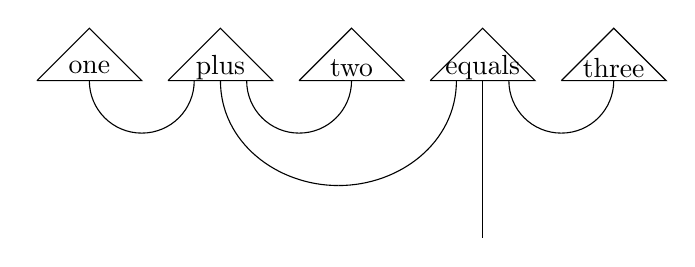
\begin{tikzpicture}[baseline=(O.base), scale=0.666]
\node (O) at (0, 0) {};
\draw (0.0, 0) -- (2.0, 0) -- (1.0, 1) -- (0.0, 0);
\node () at (1.0, 0.25) {one};
\draw (2.5, 0) -- (4.5, 0) -- (3.5, 1) -- (2.5, 0);
\node () at (3.5, 0.25) {plus};
\draw (5.0, 0) -- (7.0, 0) -- (6.0, 1) -- (5.0, 0);
\node () at (6.0, 0.25) {two};
\draw (7.5, 0) -- (9.5, 0) -- (8.5, 1) -- (7.5, 0);
\node () at (8.5, 0.25) {equals};
\draw (10.0, 0) -- (12.0, 0) -- (11.0, 1) -- (10.0, 0);
\node () at (11.0, 0.25) {three};
\draw [out=-90, in=180] (1.0, 0) to (2.0, -1);
\draw [out=-90, in=0] (3.0, 0) to (2.0, -1);
\draw [out=-90, in=180] (4.0, 0) to (5.0, -1);
\draw [out=-90, in=0] (6.0, 0) to (5.0, -1);
\draw [out=-90, in=180] (9.0, 0) to (10.0, -1);
\draw [out=-90, in=0] (11.0, 0) to (10.0, -1);
\draw [out=-90, in=180] (3.5, 0) to (5.75, -2);
\draw [out=-90, in=0] (8.0, 0) to (5.75, -2);
\draw [out=-90, in=90] (8.5, 0) to (8.5, -3);
\end{tikzpicture}

\end{center}
\end{example}

\begin{example}
For any monoidal category $\mathbf{C}$, there is a free rigid category $A(\mathbf{C})$ with a fully-faithful monoidal functor $\mathbf{C} \injects A(\mathbf{C})$, see \cite{Delpeuch14a}.
Concretely, this means that in a rigid diagram with boxes coming from a monoidal category, if the domain and codomain have no adjoint types then all snakes can be removed.
This allows to give a semantics to a pregroup grammar $G$ as a rigid functor $F : \mathbf{G} \to A(\mathbf{C})$.
For example, let $\text{one, two} : 1 \to n$ and $\text{plus} : n \times n \to n$ be functions, then we can compute the meaning of ``one plus two'':
\begin{center}
\begin{tikzpicture}[baseline=(O.base), scale=0.666]
\node (O) at (0, 3.5) {};
\node [scale=0.8] () at (0.5, 6.05) {$n$};
\node [scale=0.8] () at (2.5, 5.05) {$n^r$};
\node [scale=0.8] () at (4.5, 5.05) {$n$};
\node [scale=0.8] () at (6.5, 4.05) {$n$};
\node [scale=0.8] () at (8.5, 4.05) {$n^l$};
\node [scale=0.8] () at (5.5, 3.05) {$n$};
\node [scale=0.8] () at (10.5, 2.05) {$n$};
\draw (0.0, 6.25) .. controls (0.0, 1.75) .. (0.0, 1.75);
\draw (3.0, 5.5) .. controls (2.0, 5.5) .. (2.0, 5.25);
\draw (3.0, 5.5) .. controls (4.0, 5.5) .. (4.0, 5.25);
\draw (2.0, 5.25) .. controls (2.0, 1.75) .. (2.0, 1.75);
\draw (4.0, 5.25) .. controls (4.0, 3.75) .. (4.0, 3.75);
\draw (7.0, 4.5) .. controls (6.0, 4.5) .. (6.0, 4.25);
\draw (7.0, 4.5) .. controls (8.0, 4.5) .. (8.0, 4.25);
\draw (6.0, 4.25) .. controls (6.0, 3.75) .. (6.0, 3.75);
\draw (8.0, 4.25) .. controls (8.0, 0.75) .. (8.0, 0.75);
\draw (5.0, 3.25) .. controls (5.0, 0.0) .. (5.0, 0.0);
\draw (10.0, 2.25) .. controls (10.0, 0.75) .. (10.0, 0.75);
\draw (0.0, 1.75) .. controls (0.0, 1.5) .. (1.0, 1.5);
\draw (2.0, 1.75) .. controls (2.0, 1.5) .. (1.0, 1.5);
\draw (8.0, 0.75) .. controls (8.0, 0.5) .. (9.0, 0.5);
\draw (10.0, 0.75) .. controls (10.0, 0.5) .. (9.0, 0.5);
\draw (-0.5, 6.25) -- (0.5, 6.25) -- (0.5, 6.75) -- (-0.5, 6.75) -- (-0.5, 6.25);
\node [scale=0.8] () at (0, 6.5) {one};
\draw (3.5, 3.25) -- (6.5, 3.25) -- (6.5, 3.75) -- (3.5, 3.75) -- (3.5, 3.25);
\node [scale=0.8] () at (5.0, 3.5) {plus};
\draw (9.5, 2.25) -- (10.5, 2.25) -- (10.5, 2.75) -- (9.5, 2.75) -- (9.5, 2.25);
\node [scale=0.8] () at (10.0, 2.5) {two};
\node () at (12.0, 3.5) {$\mapsto$};
\node [scale=0.8] () at (14.5, 5.383333333333333) {$n$};
\node [scale=0.8] () at (16.5, 3.0500000000000003) {$n$};
\node [scale=0.8] () at (15.5, 0.7166666666666668) {$n$};
\draw (14.0, 5.583333333333333) .. controls (14.0, 1.4166666666666665) .. (14.0, 1.4166666666666665);
\draw (16.0, 3.2500000000000004) .. controls (16.0, 1.4166666666666665) .. (16.0, 1.4166666666666665);
\draw (15.0, 0.9166666666666667) .. controls (15.0, 0.0) .. (15.0, 0.0);
\draw (13.5, 5.583333333333334) -- (14.5, 5.583333333333334) -- (14.5, 6.083333333333334) -- (13.5, 6.083333333333334) -- (13.5, 5.583333333333334);
\node [scale=0.8] () at (14.0, 5.833333333333334) {one};
\draw (15.5, 3.25) -- (16.5, 3.25) -- (16.5, 3.75) -- (15.5, 3.75) -- (15.5, 3.25);
\node [scale=0.8] () at (16.0, 3.5) {two};
\draw (13.5, 0.9166666666666667) -- (16.5, 0.9166666666666667) -- (16.5, 1.4166666666666667) -- (13.5, 1.4166666666666667) -- (13.5, 0.9166666666666667);
\node [scale=0.8] () at (15.0, 1.1666666666666667) {plus};
\end{tikzpicture}
 $\quad \mapsto \quad 3$
\end{center}
where the first step is snake removal and the second is function evaluation as in appendix~\ref{3-cartesian}.
\end{example}

% \section{tensor.py}\label{5-tensor}%!TEX root = ms.tex

Let $\mathbf{Mat}_\bb{S}$ be the category with objects the natural numbers and arrows $m \to n$ the matrices $[n] \times [m] \to \bb{S}$ for a commutative semiring $\bb{S}$, with Kronecker product as tensor.
$\mathbf{Mat}_\bb{S}$ is compact closed, i.e. both symmetric monoidal and rigid. It is furthermore self-dual, i.e. objects are isomorphic to their adjoints.
For $\bb{S} = \bb{B}$, we get a category equivalent to finite sets and relations with Cartesian product.
For $\bb{S} = \bb{C}$, it is equivalent to finite-dimensional complex vector spaces and linear maps with the usual tensor product.
In practice, it is more convenient to consider an equivalent category $\mathbf{Tensor}_\bb{S}$ where objects are lists of natural numbers and adjoints are given by list reversal.
Arrows $(m_1, \dots, m_k) \to (n_1, \dots, n_{k'})$ are tensors of order $k + k'$, i.e. matrices $m_1 \times \dots \times m_k \to n_1 \times \dots \times n_{k'}$.

\begin{class}\normalfont\texttt{Dim(n\_0, ..., n\_k)}
is a subclass of \py{rigid.Ty} generated by natural numbers.
\end{class}

\begin{class}\normalfont\texttt{Tensor(dom, cod, array)}
is a subclass of \py{rigid.Box} given by \py{Dim}-instances \py{dom} and \py{cod} and a \texttt{numpy} \cite{VanderWaltEtAl11} \py{array} of the appropriate shape.
\py{then} and \py{tensor} are both implemented using \py{numpy.tensordot}, \py{cups} and \py{caps} return a reshaped identity.
\end{class}

\begin{class}\normalfont\texttt{TensorFunctor(ob, ar)}
is a subclass of \py{rigid.Functor} where \py{ob} and \py{ar} are mappings from \py{Ty} to \py{Dim} and from \py{Box} to \py{Tensor} respectively.
\end{class}

\begin{remark}
All the methods of the \py{Tensor} class are writen in \normalfont{\texttt{jax.numpy}}, the subset of Python+\normalfont{\texttt{numpy}} that supports automatic differentiation with \normalfont{\texttt{jax}} \cite{Google/jax20}.
\end{remark}

\begin{example}
Tensor networks can be defined as diagrams with a functor into tensors, contraction is given by functor application. They have been applied to both condensed matter physics and machine learning, see \cite{Orus14} for an introduction.
Interfacing \normalfont{DisCoPy} with tensor network tools such as \cite{KossaifiEtAl18,HauschildPollmann18,RobertsEtAl19} is left for future work.
\end{example}

\begin{example}
Relational databases can be defined as Boolean tensors: a table with $k$ columns is a state $1 \to (n_1, \dots, n_k)$ in $\mathbf{Tensor}_\bb{B}$.
Conjunctive queries are diagrams, where query containment gives the structure of a free Cartesian bicategory, see \cite{BonchiEtAl18}.
Query evaluation over a relational database is the application a functor into Boolean tensors.
\end{example}

\begin{example}\label{example-discocat}
The distributional compositional (DisCo) models of Coecke et al.
\cite{ClarkEtAl08,ClarkEtAl10} can be defined as functors
$F : \mathbf{G} \to \mathbf{Tensor}_\bb{S}$ from the rigid category $\mathbf{G}$ generated by
a pregroup grammar (see example~\ref{example-pregroup}) into tensors, i.e. they map pregroup types $t \in \mathbf{G}$ to dimensions $F(t) \in \bb{N}^\star$ and dictionnary entries $w \to t$ to tensors of shape $F(t)$.
When $F(s) = 1$, the meaning for a grammatical sentence $g : w_1 \dots w_n \to s$ is a scalar $F(g) \in \bb{S}$ which can be computed as the contraction of a tensor network.
DisCo models into real vector spaces, i.e. with $\bb{S} = \bb{R}$, received experimental support, see \cite{GrefenstetteSadrzadeh11,KartsaklisEtAl12,KartsaklisEtAl13}.
Relational DisCo models, i.e. with $\bb{S} = \bb{B}$, have been applied to question answering, see \cite{CoeckeEtAl18a, DeFeliceEtAl19a}.
\end{example}

% \section{circuit.py}\label{6-circuit}%!TEX root = ms.tex

Quantum circuits are a standard model for quantum computation.
They form the arrows of a PROP, i.e. a symmetric monoidal category generated by one object, called a qubit.
We define $\mathbf{Circ}$ as the free PROP generated by
$n$-qubit gates $g : n \to n$,
scalars $\{s : 0 \to 0\}_{s \in \bb{C}}$,
post-selection $\{\mathtt{bra}_i : 1 \to 0\}_{i \in \{0, 1\}}$
and preparation $\{\mathtt{ket}_i : 0 \to 1\}_{i \in \{0, 1\}}$ of ancilla qubits in the computational basis.
Circuit evaluation is defined as a monoidal functor $\mathtt{eval} : \mathbf{Circ} \to \mathbf{Tensor}_\bb{C}$ which sends each gate $g : n \to n$ to its unitary matrix $\mathtt{eval}(g) : 2^n \to 2^n$.

Given the circuit for an $n$-qubit state $c : 0 \to n$, measurement results are a tensor $\mathtt{measure}(c) : 1 \to 2^n$ of non-negative reals in $\mathbf{Tensor}_{\bb{R}^+}$, computed using the Born rule.
Note that if a circuit contains scalars or post selection, the measurement results need not be a normalised probability distribution.

The quotient $\mathbf{Circ}_\sim$, where $c = c'$ iff $\mathtt{eval}(c) = \mathtt{eval}(c')$, is a compact-closed category.
Cups and caps are given by the (unnormalised) Bell effect and state, the snake equation implies the correctness of the teleportation protocol.
See \cite{CoeckeKissinger17} for an introduction to diagrammatic reasoning and quantum processes.

\begin{class}\normalfont\texttt{Circuit(dom, cod, boxes, offsets)}
is a subclass of \py{rigid.Diagram} with \py{PRO}-instances as \py{dom} and \py{cod}. It has methods \py{eval}, implemented as a \py{TensorFunctor}, and \py{measure} which computes the Born rule.
\end{class}

\begin{class}\normalfont\texttt{Bra(b\_0, ..., b\_n)} and \normalfont\texttt{Ket(b\_0, ..., b\_n)} are
subclasses of \py{Circuit} and \py{rigid.Box} given by a bitstring \py{b\_0, ..., b\_n}.
\end{class}

\begin{class}\normalfont\texttt{Gate(name, n\_qubits, array)}
is a subclass of \py{Circuit} and \py{rigid.Box} with instances \py{H}, \py{CX}, \py{SWAP}, etc. Phases are implemented as subclasses \py{Rx} and \py{Rz}.
\end{class}

\begin{class}\normalfont\texttt{CircuitFunctor(ob, ar)}
is a subclass of \py{rigid.Functor} where \py{ob} and \py{ar} are mappings from \py{Ty} to \py{PRO} and from \py{Box} to \py{Circuit} respectively.
\end{class}

The methods \py{to\_tk} and \py{from\_tk} translate back and forth between DisCoPy's \py{Circuit} class and that of t$\vert$ket$\rangle$ \cite{SivarajahEtAl20}, which can then be compiled and executed on quantum hardware or simplified using \texttt{pyzx} \cite{KissingervandeWetering19}.
Note that in the translation from DisCoPy diagrams to the directed acyclic graphs of t$\vert$ket$\rangle$, we treat the \py{SWAP} gate as a logical gate, i.e. it simply renames the two qubits.
In the other direction, we introduce \py{SWAP} gates whenever a t$\vert$ket$\rangle$ gate is applied to non-adjacent qubits.
Thus, \py{from\_tk(c.to\_tk())} is equal to the original circuit \py{c} up to the axioms of symmetric monoidal categories.

\begin{example}
The quantum algorithms for natural language processing (NLP) of \cite{ZengCoecke16} can be defined as rigid functors $\mathbf{G} \to \mathbf{Circ}$ from a pregroup grammar (see examples~\ref{example-pregroup} and \ref{example-discocat}) to the category of circuits.
See \cite{Coecke19} for a discussion of distributional compositional models for NLP on quantum hardware.
A proof-of-concept was implemented using \normalfont{DisCoPy}, see the notebook of the first experiments \href{https://github.com/oxford-quantum-group/discopy/blob/master/notebooks/qnlp-experiment.ipynb}{here} and \href{https://medium.com/cambridge-quantum-computing/quantum-natural-language-processing-748d6f27b31d}{there} \cite{Meichanetzidis20} for more details.
\end{example}

% \section{cartesian.py}\label{3-cartesian}%!TEX root = ms.tex

This appendix describes \py{cartesian.Diagram} and \py{PythonFunctor}, an
implementation of \emph{Lawvere theories} and their models.
We first give a short introduction to symmetric monoidal categories (SMC), PROPs and functorial semantics.

A (strict) monoidal category $\mathbf{C}$ is \emph{symmetric} when it comes equipped
with a natural transformation $\sigma_{x, y} : x \otimes y \to y \otimes x$
such that $\sigma_{y, x} \circ \sigma_{x, y} = 1_{x \otimes y}$ (involution)
and $\sigma_{x, y \otimes z} =
(1_{z} \otimes \sigma_{x, z}) \circ (\sigma_{x, y} \otimes 1_{z})$ (hexagon).
A component $\sigma_{x, y}$ is depicted as a swap of the wires for $x$ and $y$.
The free symmetric monoidal category $\mathbf{SMC}(\Sigma)$ generated by a monoidal
signature $\Sigma$ can be defined as a quotient $\mathbf{MC}(\Sigma') / \cal{S}$ of
the free monoidal category generated by the disjoint union
$\Sigma' = \Sigma + \set{\sigma_{x, y}}_{x, y \in \Sigma_0}$. The relation
$\cal{S}$ is generated by the rules for involution and naturality:
\begin{center}
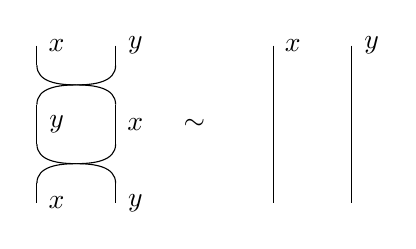
\begin{tikzpicture}[baseline=(O.base)]
\node (O) at (0, 1.0) {};
\node () at (0.25, 2.0) {$x$};
\node () at (1.25, 2.0) {$y$};
\node () at (0.25, 1.0) {$y$};
\node () at (1.25, 1.0) {$x$};
\node () at (0.25, 0.0) {$x$};
\node () at (1.25, 0.0) {$y$};
\draw [out=-90, in=90] (0, 2.0) to (0, 1.75);
\draw [out=-90, in=90] (1, 2.0) to (1, 1.75);
\draw [out=180, in=90] (0.5, 1.5) to (0.0, 1.25);
\draw [out=0, in=90] (0.5, 1.5) to (1.0, 1.25);
\draw [out=-90, in=180] (0, 1.75) to (0.5, 1.5);
\draw [out=-90, in=0] (1, 1.75) to (0.5, 1.5);
\draw [out=-90, in=90] (0.0, 1.25) to (0.0, 0.75);
\draw [out=-90, in=90] (1.0, 1.25) to (1.0, 0.75);
\draw [out=180, in=90] (0.5, 0.5) to (0.0, 0.25);
\draw [out=0, in=90] (0.5, 0.5) to (1.0, 0.25);
\draw [out=-90, in=180] (0.0, 0.75) to (0.5, 0.5);
\draw [out=-90, in=0] (1.0, 0.75) to (0.5, 0.5);
\draw [out=-90, in=90] (0.0, 0.25) to (0.0, 0.0);
\draw [out=-90, in=90] (1.0, 0.25) to (1.0, 0.0);
\node () at (2, 1.0) {$\sim$};
\node () at (3.25, 2.0) {$x$};
\node () at (4.25, 2.0) {$y$};
\draw [out=-90, in=90] (3, 2.0) to (3, 0.0);
\draw [out=-90, in=90] (4, 2.0) to (4, 0.0);
\end{tikzpicture}

\qquad and \qquad \quad
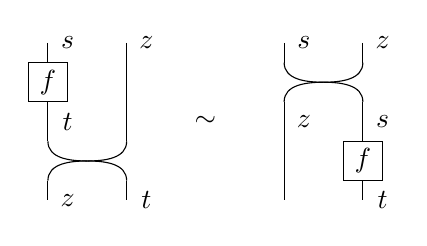
\begin{tikzpicture}[baseline=(O.base)]
\node (O) at (0, 1.0) {};
\node () at (0.25, 2.0) {$s$};
\node () at (1.25, 2.0) {$z$};
\node () at (0.25, 1.0) {$t$};
\node () at (0.25, 0.0) {$z$};
\node () at (1.25, 0.0) {$t$};
\draw [out=-90, in=90] (0, 2.0) to (0, 1.75);
\draw [out=-90, in=90] (1, 2.0) to (1, 0.75);
\draw [out=-90, in=90] (0.0, 1.25) to (0.0, 0.75);
\draw [out=180, in=90] (0.5, 0.5) to (0.0, 0.25);
\draw [out=0, in=90] (0.5, 0.5) to (1.0, 0.25);
\draw [out=-90, in=180] (0.0, 0.75) to (0.5, 0.5);
\draw [out=-90, in=0] (1, 0.75) to (0.5, 0.5);
\draw [out=-90, in=90] (0.0, 0.25) to (0.0, 0.0);
\draw [out=-90, in=90] (1.0, 0.25) to (1.0, 0.0);
\draw (-0.25, 1.25) -- (0.25, 1.25) -- (0.25, 1.75) -- (-0.25, 1.75) -- (-0.25, 1.25);
\node () at (0.0, 1.5) {$f$};
\node () at (2, 1.0) {$\sim$};
\node () at (3.25, 2.0) {$s$};
\node () at (4.25, 2.0) {$z$};
\node () at (3.25, 1.0) {$z$};
\node () at (4.25, 1.0) {$s$};
\node () at (4.25, 0.0) {$t$};
\draw [out=-90, in=90] (3, 2.0) to (3, 1.75);
\draw [out=-90, in=90] (4, 2.0) to (4, 1.75);
\draw [out=180, in=90] (3.5, 1.5) to (3.0, 1.25);
\draw [out=0, in=90] (3.5, 1.5) to (4.0, 1.25);
\draw [out=-90, in=180] (3, 1.75) to (3.5, 1.5);
\draw [out=-90, in=0] (4, 1.75) to (3.5, 1.5);
\draw [out=-90, in=90] (3.0, 1.25) to (3.0, 0.0);
\draw [out=-90, in=90] (4.0, 1.25) to (4.0, 0.75);
\draw [out=-90, in=90] (4.0, 0.25) to (4.0, 0.0);
\draw (3.75, 0.25) -- (4.25, 0.25) -- (4.25, 0.75) -- (3.75, 0.75) -- (3.75, 0.25);
\node () at (4.0, 0.5) {$f$};
\end{tikzpicture}

\end{center}
for all $x, y, z \in \Sigma_0$ and $f : s \to t$ in $\Sigma'$. Note that
$s, t \in \Sigma_0^\star$ may be of arbitrary length, in which case $\sigma_{s, z}$ and $\sigma_{t, z}$ are defined as ladders of swaps,
i.e. the symmetry for compound types $\sigma_{x \otimes y, z}$ and
$\sigma_{x, y \otimes z}$ is defined inductively by:
\begin{center}
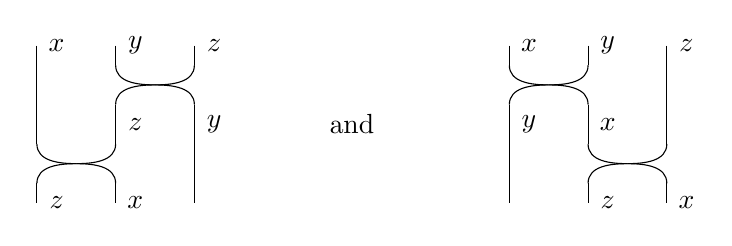
\begin{tikzpicture}[baseline=(O.base)]
\node (O) at (0, 1.0) {};
\node () at (0.25, 2.0) {$x$};
\node () at (1.25, 2.0) {$y$};
\node () at (2.25, 2.0) {$z$};
\node () at (1.25, 1.0) {$z$};
\node () at (2.25, 1.0) {$y$};
\node () at (0.25, 0.0) {$z$};
\node () at (1.25, 0.0) {$x$};
\draw [out=-90, in=90] (0, 2.0) to (0, 0.75);
\draw [out=-90, in=90] (1, 2.0) to (1, 1.75);
\draw [out=-90, in=90] (2, 2.0) to (2, 1.75);
\draw [out=180, in=90] (1.5, 1.5) to (1.0, 1.25);
\draw [out=0, in=90] (1.5, 1.5) to (2.0, 1.25);
\draw [out=-90, in=180] (1, 1.75) to (1.5, 1.5);
\draw [out=-90, in=0] (2, 1.75) to (1.5, 1.5);
\draw [out=-90, in=90] (1.0, 1.25) to (1.0, 0.75);
\draw [out=-90, in=90] (2.0, 1.25) to (2.0, 0.0);
\draw [out=180, in=90] (0.5, 0.5) to (0.0, 0.25);
\draw [out=0, in=90] (0.5, 0.5) to (1.0, 0.25);
\draw [out=-90, in=180] (0, 0.75) to (0.5, 0.5);
\draw [out=-90, in=0] (1.0, 0.75) to (0.5, 0.5);
\draw [out=-90, in=90] (0.0, 0.25) to (0.0, 0.0);
\draw [out=-90, in=90] (1.0, 0.25) to (1.0, 0.0);
\node () at (4, 1.0) {and};
\node () at (6.25, 2.0) {$x$};
\node () at (7.25, 2.0) {$y$};
\node () at (8.25, 2.0) {$z$};
\node () at (6.25, 1.0) {$y$};
\node () at (7.25, 1.0) {$x$};
\node () at (7.25, 0.0) {$z$};
\node () at (8.25, 0.0) {$x$};
\draw [out=-90, in=90] (6, 2.0) to (6, 1.75);
\draw [out=-90, in=90] (7, 2.0) to (7, 1.75);
\draw [out=-90, in=90] (8, 2.0) to (8, 0.75);
\draw [out=180, in=90] (6.5, 1.5) to (6.0, 1.25);
\draw [out=0, in=90] (6.5, 1.5) to (7.0, 1.25);
\draw [out=-90, in=180] (6, 1.75) to (6.5, 1.5);
\draw [out=-90, in=0] (7, 1.75) to (6.5, 1.5);
\draw [out=-90, in=90] (6.0, 1.25) to (6.0, 0.0);
\draw [out=-90, in=90] (7.0, 1.25) to (7.0, 0.75);
\draw [out=180, in=90] (7.5, 0.5) to (7.0, 0.25);
\draw [out=0, in=90] (7.5, 0.5) to (8.0, 0.25);
\draw [out=-90, in=180] (7.0, 0.75) to (7.5, 0.5);
\draw [out=-90, in=0] (8, 0.75) to (7.5, 0.5);
\draw [out=-90, in=90] (7.0, 0.25) to (7.0, 0.0);
\draw [out=-90, in=90] (8.0, 0.25) to (8.0, 0.0);
\end{tikzpicture}

\end{center}
The symmetry for the empty type is defined to be the identity
$\sigma_{x, 1} = \sigma_{1, x} = 1_x$.
% Thus, the hexagon identity holds on the nose. Picking $f = \sigma_{x, y}$ in
% the naturality rule yields the Yang-Baxter identity:
% \begin{center}
% 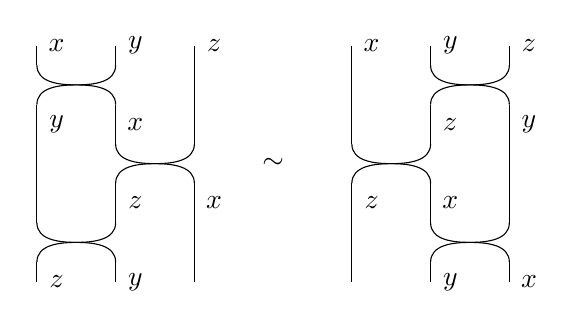
\begin{tikzpicture}[baseline=(O.base)]
\node (O) at (0, 1.5) {};
\node () at (0.25, 3.0) {$x$};
\node () at (1.25, 3.0) {$y$};
\node () at (2.25, 3.0) {$z$};
\node () at (0.25, 2.0) {$y$};
\node () at (1.25, 2.0) {$x$};
\node () at (1.25, 1.0) {$z$};
\node () at (2.25, 1.0) {$x$};
\node () at (0.25, 0.0) {$z$};
\node () at (1.25, 0.0) {$y$};
\draw [out=-90, in=90] (0, 3.0) to (0, 2.75);
\draw [out=-90, in=90] (1, 3.0) to (1, 2.75);
\draw [out=-90, in=90] (2, 3.0) to (2, 1.75);
\draw [out=180, in=90] (0.5, 2.5) to (0.0, 2.25);
\draw [out=0, in=90] (0.5, 2.5) to (1.0, 2.25);
\draw [out=-90, in=180] (0, 2.75) to (0.5, 2.5);
\draw [out=-90, in=0] (1, 2.75) to (0.5, 2.5);
\draw [out=-90, in=90] (0.0, 2.25) to (0.0, 0.75);
\draw [out=-90, in=90] (1.0, 2.25) to (1.0, 1.75);
\draw [out=180, in=90] (1.5, 1.5) to (1.0, 1.25);
\draw [out=0, in=90] (1.5, 1.5) to (2.0, 1.25);
\draw [out=-90, in=180] (1.0, 1.75) to (1.5, 1.5);
\draw [out=-90, in=0] (2, 1.75) to (1.5, 1.5);
\draw [out=-90, in=90] (1.0, 1.25) to (1.0, 0.75);
\draw [out=-90, in=90] (2.0, 1.25) to (2.0, 0.0);
\draw [out=180, in=90] (0.5, 0.5) to (0.0, 0.25);
\draw [out=0, in=90] (0.5, 0.5) to (1.0, 0.25);
\draw [out=-90, in=180] (0.0, 0.75) to (0.5, 0.5);
\draw [out=-90, in=0] (1.0, 0.75) to (0.5, 0.5);
\draw [out=-90, in=90] (0.0, 0.25) to (0.0, 0.0);
\draw [out=-90, in=90] (1.0, 0.25) to (1.0, 0.0);
\node () at (3, 1.5) {$\sim$};
\node () at (4.25, 3.0) {$x$};
\node () at (5.25, 3.0) {$y$};
\node () at (6.25, 3.0) {$z$};
\node () at (5.25, 2.0) {$z$};
\node () at (6.25, 2.0) {$y$};
\node () at (4.25, 1.0) {$z$};
\node () at (5.25, 1.0) {$x$};
\node () at (5.25, 0.0) {$y$};
\node () at (6.25, 0.0) {$x$};
\draw [out=-90, in=90] (4, 3.0) to (4, 1.75);
\draw [out=-90, in=90] (5, 3.0) to (5, 2.75);
\draw [out=-90, in=90] (6, 3.0) to (6, 2.75);
\draw [out=180, in=90] (5.5, 2.5) to (5.0, 2.25);
\draw [out=0, in=90] (5.5, 2.5) to (6.0, 2.25);
\draw [out=-90, in=180] (5, 2.75) to (5.5, 2.5);
\draw [out=-90, in=0] (6, 2.75) to (5.5, 2.5);
\draw [out=-90, in=90] (5.0, 2.25) to (5.0, 1.75);
\draw [out=-90, in=90] (6.0, 2.25) to (6.0, 0.75);
\draw [out=180, in=90] (4.5, 1.5) to (4.0, 1.25);
\draw [out=0, in=90] (4.5, 1.5) to (5.0, 1.25);
\draw [out=-90, in=180] (4, 1.75) to (4.5, 1.5);
\draw [out=-90, in=0] (5.0, 1.75) to (4.5, 1.5);
\draw [out=-90, in=90] (4.0, 1.25) to (4.0, 0.0);
\draw [out=-90, in=90] (5.0, 1.25) to (5.0, 0.75);
\draw [out=180, in=90] (5.5, 0.5) to (5.0, 0.25);
\draw [out=0, in=90] (5.5, 0.5) to (6.0, 0.25);
\draw [out=-90, in=180] (5.0, 0.75) to (5.5, 0.5);
\draw [out=-90, in=0] (6.0, 0.75) to (5.5, 0.5);
\draw [out=-90, in=90] (5.0, 0.25) to (5.0, 0.0);
\draw [out=-90, in=90] (6.0, 0.25) to (6.0, 0.0);
\end{tikzpicture}

% \end{center}
An SMC where the tensor is the Cartesian product and the unit is terminal
(i.e. a category with finite products) is called a \emph{Cartesian category}.
Equivalently, an SMC is Cartesian when objects carry a natural
commutative comonoid structure \cite[6.1]{Selinger10}.
Given a monoidal signature $\Sigma$, the free Cartesian category
$\mathbf{CC}(\Sigma)$ is the quotient
$\mathbf{MC}(\Sigma'') / (\cal{S} + \cal{P})$ for
$\Sigma'' = \Sigma' + \set{\mu_{x} : x \to x \otimes x}_{x \in \Sigma_0} + \set{\epsilon_x : x \to 1}_{x \in \Sigma_0}$.
The components $\mu_{x}$ and $\epsilon_{x}$ are depicted as wire splitting and
ending respectively. The comonoids of non-atomic
types inductively. That for the unit is the identity and the comonoid
of $x \otimes y$ is given by:
\begin{center}
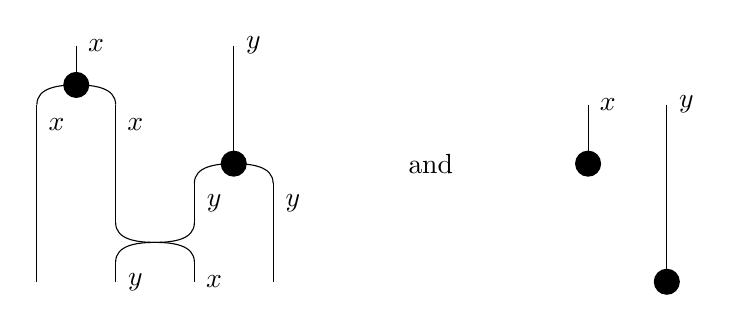
\begin{tikzpicture}[baseline=(O.base)]
\node (O) at (0, 1.5) {};
\node () at (0.75, 3.0) {$x$};
\node () at (2.75, 3.0) {$y$};
\node () at (0.25, 2.0) {$x$};
\node () at (1.25, 2.0) {$x$};
\node () at (2.25, 1.0) {$y$};
\node () at (3.25, 1.0) {$y$};
\node () at (1.25, 0.0) {$y$};
\node () at (2.25, 0.0) {$x$};
\draw [out=-90, in=90] (0.5, 3.0) to (0.5, 2.75);
\draw [out=-90, in=90] (2.5, 3.0) to (2.5, 1.75);
\draw [out=180, in=90] (0.5, 2.5) to (0.0, 2.25);
\draw [out=0, in=90] (0.5, 2.5) to (1.0, 2.25);
\draw [out=-90, in=90] (0.5, 2.75) to (0.5, 2.5);
\draw [out=-90, in=90] (0.0, 2.25) to (0.0, 0.0);
\draw [out=-90, in=90] (1.0, 2.25) to (1.0, 0.75);
\draw [out=180, in=90] (2.5, 1.5) to (2.0, 1.25);
\draw [out=0, in=90] (2.5, 1.5) to (3.0, 1.25);
\draw [out=-90, in=90] (2.5, 1.75) to (2.5, 1.5);
\draw [out=-90, in=90] (2.0, 1.25) to (2.0, 0.75);
\draw [out=-90, in=90] (3.0, 1.25) to (3.0, 0.0);
\draw [out=180, in=90] (1.5, 0.5) to (1.0, 0.25);
\draw [out=0, in=90] (1.5, 0.5) to (2.0, 0.25);
\draw [out=-90, in=180] (1.0, 0.75) to (1.5, 0.5);
\draw [out=-90, in=0] (2.0, 0.75) to (1.5, 0.5);
\draw [out=-90, in=90] (1.0, 0.25) to (1.0, 0.0);
\draw [out=-90, in=90] (2.0, 0.25) to (2.0, 0.0);
\node [circle, fill=black] () at (0.5, 2.5) {};
\node [circle, fill=black] () at (2.5, 1.5) {};
\node () at (5.0, 1.5) {and};
\node () at (7.25, 2.25) {$x$};
\node () at (8.25, 2.25) {$y$};
\draw [out=-90, in=90] (7.0, 2.25) to (7.0, 1.75);
\draw [out=-90, in=90] (8.0, 2.25) to (8.0, 0.25);
\draw [out=-90, in=90] (7.0, 1.75) to (7.0, 1.5);
\draw [out=-90, in=90] (8.0, 0.25) to (8.0, 0.0);
\node [circle, fill=black] () at (7.0, 1.5) {};
\node [circle, fill=black] () at (8.0, 0.0) {};
\end{tikzpicture}

\end{center}
The relation $(\cal{S} + \cal{P})$ is given by the axioms for commutative
comonoids plus naturality of symmetry, coproduct and counit for each generating
arrow.
A \emph{PROP} (PROduct and Permutation) \cite{Lack04} is an SMC generated by one object, a \emph{Lawvere theory} \cite{Lawvere63} is a Cartesian category generated one object.

Lawvere theories are implemented by the class \py{cartesian.Diagram}, a subclass of \linebreak \py{monoidal.Diagram} with static methods \py{swap}, \py{copy} and \py{delete} implementing the structural morphisms.
\py{cartesian.Box} is a subclass of \py{monoidal.Box} where each instance holds a Python function with natural numbers as domain and codomain. A Cartesian box \py{f} with \py{f.dom, f.cod == (m, n)} sends $m$-tuples to $n$-tuples, it can be defined in the standard syntax for Python functions using the decorator \py{@disco(m, n)}.
\py{Swap}, \py{Copy} and \py{Del} are subclasses of \py{cartesian.Box} which implement the symmetry and comonoid on the generating object.
\py{cartesian.Functor} is a subclass of \py{monoidal.Functor} which preserves symmetry and product.
\py{Function} is a subclass of \py{cartesian.Box} where \py{then} and \py{tensor} are overriden by function composition and tuple concatenation.
The \py{PythonFunctor} class implements Cartesian functors into \py{Function}, i.e. it maps the formal composition of diagrams to the concrete composition of functions.
Note that when \py{f} and \py{g} have side-effects, the tensor \py{f @ g} is in
general different from \py{Id(f.dom) @ g >> f @ Id(g.cod)}. Thus, \py{Function}
is closer to the implementation of a premonoidal than a monoidal category,
see example~\ref{example-2}.

\begin{example}
The Lawvere theory $\mathbf{F}$ with no generating arrows is the
opposite of the category of finite sets with disjoint union as monoidal structure: diagrams $f : m \to n$ in
$\mathbf{F}$ correspond precisely to the graphs of the functions $f : [n] \to [m]$.
The subcategories of diagrams in $\mathbf{F}$ with no coproduct, no counit and no symmetry correspond to injective, surjective and monotone functions respectively.
The subcategory of $\mathbf{F}$ generated by symmetry alone, i.e. the free SMC generated by one object, corresponds to bijections.
The normal form for diagrams in $\mathbf{F}$ is given by decomposing any function into a surjection and a monotone injection, see \cite[Theorem~3]{Lafont03}.
\end{example}

\begin{example}
For a semiring $\bb{S}$, the category of matrices over $\bb{S}$ with direct sum as monoidal product can be defined as a Lawvere theory generated by a commutative monoid $+ : 2 \to 1$ with unit $e : 0 \to 1$ and scalars $\set{s : 1 \to 1}_{s \in \bb{S}}$.
The relations are given by the axioms for semirings, see \cite{WadsleyWoods15}.
The naturality relation for the comonoid with respect to $+$ and $e$ are called the bialgebra laws, they have applications in control and network theory \cite{BaezErbele14,BaezEtAl18}.
\end{example}

\begin{example}
Let $\mathbf{NN}$ be the Lawvere
theory generated by sum $+ : 2 \to 1$, activation $a : 1 \to 1$,
finite sets of weights $\set{w_i : 1 \to 1}_{i \in W}$ and biases
$\set{b_i : 0 \to 1}_{i \in B}$. The arrows of $\mathbf{NN}$ are the diagrams
of neural network architectures.
Given a set of parameters $\theta : W + B \to \bb{R}$, an implementation is
given by the model $F_\theta : \mathbf{NN} \to \mathbf{Set}$ such that
$F_\theta(1) = \bb{R}$,
$F_\theta(b_i) = \set{() \mapsto \theta(b_i)}$,
$F_\theta(w_i) = \set{x \mapsto \theta(w_i) \cdot x}$,
$F_\theta(+) = \set{(x, y) \mapsto x + y}$
and $F_\theta(a) : \bb{R} \to \bb{R}$ is a non-linearity such as sigmoid.
A loss $l : (\bb{R}^m \to \bb{R}^n) \to \bb{R}$ for an architecture $f : m \to n$ in $\mathbf{NN}$ takes an implementation and
returns a real number encoding its success at some data-driven task.
The gradient of $\theta \mapsto l(F_\theta(f))$ can be computed by
back-propagation over the architecture $f$, using automatic differentiation tools such as $\mathtt{jax}$ \cite{Google/jax20}. The back-propagation algorithm is
itself part of a functor $\mathbf{NN} \to \mathbf{Learn}$, where $\mathbf{Learn}$ is a
Cartesian category of supervised learning algorithms, see \cite{FongEtAl17, FongJohnson19}.
\end{example}

% \section{drawing.py}\label{a-draw}%!TEX root = ms.tex

We reformulate some of the definitions and results from Joyal, Street \cite{JoyalStreet88}.

\begin{definition}
A \emph{topological graph}, also called 1d cell complex, is a tuple $(\Gamma, \Gamma_0, \Gamma_1)$ of a Hausdorff space $\Gamma$ and a closed, discrete subset $\Gamma_0 \sub \Gamma$ of nodes such that $\Gamma - \Gamma_0 = \bigsqcup \Gamma_1$ is the sum of its connected components $\Gamma_1$, called edges, each homeomorphic to an open intervals with boundary in $\Gamma_0$.
\end{definition}

\begin{definition}
A planar graph between two real numbers $a < b$ is a finite topological graph $\Gamma$ embedded in $\bb{R} \times [a, b]$ such that every $x \in \Gamma \cap (\bb{R} \times \set{a, b})$ is a node in $\Gamma_0$ and belongs to the closure of exactly one edge in $\Gamma_1$.
\end{definition}

The points in $\Gamma_0 \cap (\bb{R} \times \set{a, b})$ are called outer nodes,
they are the boundary of the domain and codomain $\mathtt{dom}(\Gamma), \mathtt{cod}(\Gamma) \in \Gamma_1^\star$ of the planar graph $\Gamma$.
The points $f \in \Gamma_0 - (\bb{R} \times \set{a, b})$ are called inner nodes, they have a domain and codomain $\mathtt{dom}(f), \mathtt{cod}(f) \in \Gamma_1^\star$ given by the edges that have $f$ as boundary.
The composition $\Gamma \circ \Gamma'$ and tensor $\Gamma \otimes \Gamma'$ are defined by rescaling and pasting the two planar graphs $\Gamma, \Gamma'$ vertically and horizontally respectively, see \cite[§4]{JoyalStreet88}.

A planar graph $\Gamma$ is \emph{progressive}, or recumbent, when the second projection $e \to [a, b]$ is injective for every edge $e \in \Gamma_1$. Progressive planar graphs have no cups or caps.
A progressive planar graph is \emph{generic} when the projection $\Gamma_0 - (\bb{R} \times \set{a, b}) \to (a, b)$ is injective, i.e. there are no two inner nodes at the same height.
A deformation of planar graphs is a continuous map $h : \Gamma \times [0, 1] \to [a, b] \times \bb{R}$ such that 1) for all $t \in [0, 1]$, $h(-, t)$ is an embedding whose image is a planar graph, and 2) for all $x \in \Gamma_0$, if $h(x, t)$ is inner for some $t$ then it is inner for all values of $t \in [0, 1]$.
A deformation of planar graphs is progressive (generic) when for all $t \in [0, 1]$, $h(-, t)$ is progressive (generic).

The induced equivalence relation --- with $\Gamma_0 \sim \Gamma_1$ if and only if there is a deformation $h$ with $h(-, 0) = \Gamma_0$ and $h(-, 1) = \Gamma_1$ --- is a congruence with respect to composition and tensor of planar graphs,
i.e. if $\Gamma_0 \sim \Gamma_1$ and $\Omega_0 \sim \Omega_1$ then $\Gamma_0 \otimes \Omega_0 \sim \Gamma_1 \otimes \Omega_1$ and $\Gamma_0 \circ \Omega_0 \sim \Gamma_1 \circ \Omega_1$.
Furthermore, tensor and composition are associative and they respect the interchange law up to progessive deformation.
Thus, progessive planar graphs up to progessive deformation form a strict monoidal category \cite[Proposition~4]{JoyalStreet88}.

Given a monoidal signature $\Sigma$, a \emph{valuation} $v$ of a planar graph $\Gamma$ is a pair of functions $v_0 : \Gamma_1 \to \Sigma_0$ and $v_1 : \Gamma_0 - (\bb{R} \times \set{a, b}) \to \Sigma_1$ that send edges to objects and inner nodes to arrows, which commute with domain and codomain.
Progressive planar graphs valued in $\Sigma$ (up to progressive deformation) are the free monoidal category \cite[Theorem~5]{JoyalStreet88}.
We conjecture that generic planar graphs up to generic deformation are the free premonoidal category.

From the universal property, we know that the category of progressive planar graph is equivalent to the combinatorial definition of free monoidal categories given in section~\ref{2-monoidal}.
Concretely, this equivalence is witnessed by the following pair of algorithms translating between planar graphs and diagrams.

\vspace{-5pt}
\begin{algorithm}
\SetKwInOut{Input}{Input}\SetKwInOut{Output}{Output}
\Input{A progressive planar graph $\Gamma$}
\Output{\py{Diagram(dom, cod, boxes, offsets)}}
\BlankLine
\DontPrintSemicolon
Compute the connected components $\Gamma_1$ and their boundaries $\Gamma_0$.\;
Order the nodes by height and partition them into $\Gamma_0 = \py{dom} + \py{boxes} + \py{cod}$.\;
Find the start and end points $\Gamma_1 \to (\py{dom} + \py{boxes}) \times (\py{boxes} + \py{cod})$ for each edge, the preimage of this map gives the domain and codomain for each box.\;
Compute $\py{offsets}$ as the number of edges to the left of each box.\;
\caption{read}
\end{algorithm}
\vspace{-22pt}
\begin{algorithm}
\SetKwInOut{Input}{Input}\SetKwInOut{Output}{Output}
\Input{\py{Diagram(dom, cod, boxes, offsets)}}
\Output{A progressive planar graph $\Gamma$}
\BlankLine
\DontPrintSemicolon
Set $\Gamma_0 := \set{(i, 0) \ \vert \ i < \py{len(dom)}}$ and $\Gamma_1 := \emptyset$.\;
\For{\py{height, (box, offset) in enumerate(zip(boxes, offsets))}}{
Deform $\Gamma$ so that there is at least \py{len(box.cod) + 1} horizontal space between the edges of $\mathtt{cod}(\Gamma)$ at index \py{offset} and \py{offset + len(box.dom)}.\label{step-3}\;
Set $\Gamma_0 := \Gamma_0 + \{\py{box}\}$ for $\py{box} = (m, \py{height} +\frac{1}{2})$ with $m$ computed at step~\ref{step-3} and $\Gamma_1 := \Gamma_1 + \{x \to \py{box} \ \vert \ x \in
\py{box.dom}\} + \{\py{box} \to x \ \vert \ x \in
\py{box.cod}\}$.
}
Return $\Gamma := \Gamma + \{(i, j) \to (i, \py{max(len(boxes), 1)}) \ \vert \ (i, j) \in \mathtt{cod}(\Gamma)\}$.
\caption{draw}
\end{algorithm}


\chapter{Quantum natural language processing}

\chapter{Diagrammatic differentiation}

% %!TEX root = main.tex

\begin{abstract}
We introduce diagrammatic differentiation for tensor calculus by generalising the
dual number construction from rigs to monoidal categories. Applying this to ZX
diagrams, we show how to calculate diagrammatically the gradient of a linear map
with respect to a phase parameter. For diagrams of parametrised quantum circuits,
we get the well-known parameter-shift rule at the basis of many variational
quantum algorithms. We then extend our method to the automatic
differentation of hybrid classical-quantum circuits, using diagrams with bubbles
to encode arbitrary non-linear operators. Moreover, diagrammatic differentiation
comes with an open-source implementation in DisCoPy, the Python library for
monoidal categories.
Diagrammatic gradients of classical-quantum circuits can then be simplified
using the PyZX library and executed on quantum hardware via the
tket compiler. This opens the door to many practical applications
harnessing both the structure of string diagrams and the computational power of
quantum machine learning.
\end{abstract}

\section*{Introduction}

String diagrams are a graphical language introduced by Penrose \cite{Penrose71}
to manipulate tensor expressions: wires represent vector spaces, nodes represent
multi-linear maps between them. In \cite{PenroseRindler84}, these diagrams are
used to describe the geometry of space-time and an extra piece of notation is
introduced: the covariant derivative is represented as a bubble around the tensor
to be differentiated. Joyal and Street \cite{JoyalStreet88,JoyalStreet91}
characterised string diagrams as the arrows of free monoidal categories, however
their geometry of tensor calculus makes no mention of differential calculus, it
only deals with composition and tensor.

In categorical quantum mechanics \cite{AbramskyCoecke08} string diagrams
are used to axiomatise quantum theory in terms of dagger compact-closed
categories. This culminated in the ZX-calculus \cite{CoeckeDuncan08},
a graphical language that provides a complete set of rules for qubit quantum
computing \cite{JeandelEtAl18a,HadzihasanovicEtAl18}. ZX diagrams
have recently been used for state-of-the-art quantum circuit optimisation
\cite{KissingerVanDeWetering20,DuncanEtAl20,DeBeaudrapEtAl20}, compilation
\cite{CowtanEtAl20,DeGriendDuncan20}, extraction \cite{BackensEtAl20} and error
correction \cite{ChancellorEtAl18,GidneyFowler19}. In recent work, ZX diagrams
have been used to study quantum machine learning \cite{Yeung20,ZhaoGao21} and
its application to quantum natural language processing
\cite{MeichanetzidisEtAl20a,CoeckeEtAl20}.

In this work, we introduce diagrammatic differentiation: a graphical notation
for manipulating tensor derivatives. On the theoretical side, we generalise
the dual number construction (discussed in section~\ref{1-dual-numbers})
from rigs to monoidal categories (section~\ref{2-dual-diagrams}). We then apply
this construction to the category of ZX diagrams (section~\ref{2b-differentiating-zx})
and of quantum circuits (section~\ref{3-dual-circuits}). In section~\ref{4-bubbles}
we give a formal definition of diagrams with bubbles and their gradient with the
chain rule. We use this to differentiate quantum circuits with neural
networks as classical post-processing. The theory comes with an
implementation in DisCoPy \cite{DeFeliceEtAl20}, the Python library for
monoidal categories. The gradients of classical-quantum circuits can then
be simplified using the PyZX library \cite{KissingerVanDeWetering19} and compiled
on quantum hardware via the tket compiler \cite{SivarajahEtAl20}.

\section*{Related work}

The same bubble notation for vector calculus is proposed in \cite{KimEtAl20},
but they have mainly pedagogical motivations and restrict themselves to the case
of three-dimensional Euclidean space. To the best of our knowledge, our
definition is the first formal account of string diagrams with bubbles for
tensor derivatives.

Differential categories \cite{BluteEtAl06} have been introduced to axiomatise
the notion of derivative. More recently reverse derivative categories
\cite{CockettEtAl19} generalised the notion of back-propagation, they have been
proposed as a categorical foundation for gradient-based learning
\cite{CruttwellEtAl21}. These frameworks all define the derivative
of a morphism with respect to its domain. In our setup however, we define
the derivative of parametrised morphism with respect to parameters that are
in some sense external to the category. Investigating the relationship between
these two definitions is left to future work.

% %!TEX root = main.tex

\section{Dual numbers}\label{1-dual-numbers}

Dual numbers were first introduced by Clifford in 1873 \cite{Clifford73}.
Given a commutative rig (i.e. a riNg without Negatives) $\S$, the rig of dual
numbers $\D[\S]$ extends $\S$ by adjoining a new element $\epsilon$ such that $\epsilon^2 = 0$.
Concretely, elements of $\D[\S]$ are formal sums $s + s' \epsilon$ where
$s$ and $s'$ are scalars in $\S$.
We write $\pi_0, \pi_1 : \D[\S] \to \S$
for the projection on the real and epsilon component respectively.
Addition and multiplication of dual numbers are given by:
\begin{align} \begin{split}\label{linearity}
(a + a' \ \epsilon ) + (b + b' \ \epsilon)
\quad &= \quad (a + b) \s + \s (a + b') \ \epsilon
\end{split}\\
\begin{split}\label{product-rule}
(a + a' \ \epsilon ) \times (b + b' \ \epsilon)
\quad &= \quad (a \times b) \s + \s (a \times b' \ + \ a' \times b) \ \epsilon
\end{split}
\end{align}

A related notion is that of differential rig: a rig $\S$ equipped with a
derivation, i.e. a map $\partial : \S \to \S$ which preserves sums and satisfies
the Leibniz product rule
$\partial(f \times g) = f \times \partial(g) + \partial(f) \times g$ for all
$f, g \in \S$.
An equivalent condition is that the map $f \mapsto f + (\partial f) \epsilon$
is a homomorphism of rigs $\S \to \D[\S]$. The correspondance also works the
other way around: given a homorphism $\partial : \S \to \D[\S]$ such that
$\pi_0 \circ \partial = \id_\S$, projecting on the epsilon component is a
derivation $\pi_1 \circ \partial : \S \to \S$. The motivating example is the rig
of smooth functions $\S = \R \to \R$, where differentiation is a derivation.
Concretely, we can extend any smooth function $f : \R \to \R$ to a
function $f : \D[\R] \to \D[\R]$ over the dual numbers defined by:
\begin{equation}\label{dual-numbers-eq}
f(a + a' \epsilon) \quad = \quad f(a) \s + \s a' \times (\partial f)(a) \epsilon
\end{equation}

We can use equations~\ref{linearity}, \ref{product-rule} and \ref{dual-numbers-eq}
to derive the usual rules for gradients in terms of dual numbers.
For the identity function we have $\id(a + a' \epsilon) = \id(a) + a' \epsilon$,
i.e. $\partial \id = 1$. For the constant functions we have $c(a + a' \epsilon) =
c(a) + 0 \epsilon$, i.e. $\partial c = 0$.
For addition, multiplication and composition of functions, we can derive the
following \emph{linearity}, \emph{product} and \emph{chain} rules:
\begin{align} \begin{split}
    (f + g)(a + a' \epsilon)
    \s &= \s (f + g)(a) \s + \s a' \times (\partial f + \partial g)(a) \epsilon
\end{split}\\ \begin{split}
    (f \times g)(a + a' \epsilon)
    \s &= \s (f \times g)(a) \s + \s a' \times (f \times \partial g \ + \ \partial f \times g)(a) \epsilon
\end{split}\\ \begin{split}
    (f \circ g)(a + a' \epsilon)
    \s &= \s (f \circ g)(a) \s + \s a' \times (\partial g \ \times \ \partial f \circ g)(a) \epsilon
\end{split} \end{align}

This generalises to smooth functions $\R^n \to \R^m$, where the partial
derivative $\partial_i$ is a derivation for each $i < n$.
The functions $\F_2^n \to \F_2^m$ on the two-element
field $\F_2$ with elementwise XOR as sum and conjunction as product
also forms a differential rig.
The partial derivative is given by $(\partial_i f)(\vec{x}) =
f(\vec{x}_{[x_i \mapsto 0]}) \oplus f(\vec{x}_{[x_i \mapsto 1]})$.
Intuitively, the $\F_2$ gradient $\partial_i f(\vec{x}) \in \F_2^m$ encodes
which coordinates of $f(\vec{x})$ actually depend on the input $x_i$.
An example of differential rig that isn't also a ring is given by the set
$\N[X]$ of polynomials with natural number coefficients, again each
partial derivative is a derivation.

A more exotic example is the rig of Boolean functions with elementwise
disjunction as sum and conjunction as product. Boolean functions $\B^n \to \B^m$
can be represented as tuples of $m$ propositional formulae over $n$ variables.
The partial derivative $\partial_i$ for $i < n$ is defined by induction over
the formulae: for variables we have $\partial_i x_j = \delta_{ij}$,
for constants $\partial_i 0 = \partial_i 1 = 0$ and for negation
$\partial_i \neg \phi = \neg \partial_i \phi$. The derivative of disjunctions
and conjunctions are given by the linerarity and product rules.
Equivalently, the gradient of a propositional formula can be given by
$\partial_i \phi = \neg \phi_{[x_i \mapsto 0]} \land \phi_{[x_i \mapsto 1]}$.
Concretely, a model satisfies $\partial_i \phi$ if and only if it satisfies
$\phi \leftrightarrow x_i$: the derivative is true when the variable and the
formula are positively correlated. Substituting $x_i$ with its negation,
we get that a model satisfies $\partial_i \phi_{[x_i \mapsto \neg x_i]}$
if and only if it satisfies $\phi \leftrightarrow \neg x_i$, i.e. iff variable
and formula are anti-correlated.
Note that although $\B$ and $\F_2$ are isomorphic as sets, they are distinct
rigs. Their derivations are related however by $\partial^{\F_2}_i f \mapsto
\partial^\B_i \phi \lor \partial^\B_i \phi_{[x_i \mapsto \neg x_i]}$
for $\phi : \B^n \to \B$ the formula corresponding to the function
$f : \F_2^n \to \F_2$. That is, a Boolean function depends on an input variable
precisely when either the corresponding formula is positively correlated or
anti-correlated.

Dual numbers are a fundamental tool for \emph{automatic differentiation}
\cite{Hoffmann16}, i.e.
they allow to compute the derivative of a function automatically from its
definition. The key idea is that given a definition of $f : \S^n \to \S^m$ as a
composition of elementary functions, we can compute $(\partial_i f)(a)$ by
evaluating $f(a + \epsilon)$ and projecting on the epsilon component.

% %!TEX root = main.tex

\section{Dual diagrams}\label{2-dual-diagrams}

Our main technical contribution is to generalise derivations from rigs to
monoidal categories with sums. Applying this to free monoidal categories,
where the arrows are string diagrams, we say a derivation is diagrammatic
when it commutes with the interpretation of the diagrams. We take two
different flavours of the ZX-calculus as our main examples.

Let $(\mathbf{C}, \otimes, 1)$ be a monoidal category with sums, i.e.
it has commutative monoids on each homset $(+) : \prod_{x,y}
\mathbf{C}(x, y) \times \mathbf{C}(x, y) \to \mathbf{C}(x, y)$
with unit $0 \in \prod_{x,y} \mathbf{C}(x, y)$
such that composition and tensor distribute over the sum.
Note that a one-object monoidal category with sums is simply a rig.
Our motivating example is the category $\mathbf{Mat}_\S$ with natural numbers
as objects and matrices valued in a commutative rig $\S$ as arrows, with matrix
multiplication as composition, Kronecker product as tensor and entrywise sum.
We define the category $\D[\mathbf{C}]$ by adjoining a scalar (i.e. an
endomorphism of the monoidal unit) $\epsilon$ such that $\epsilon \otimes \epsilon = 0$\footnote{
Note that in the case when $\mathbf{C}$ is not symmetric monoidal (or at least braided) the axiom $\epsilon \otimes f = f \otimes \epsilon$ is also needed.
}.
Concretely, the objects of $\D[\mathbf{C}]$ are the same as those of $\mathbf{C}$, the arrows
are given by formal sums $f + f' \epsilon$ of parallel arrows $f, f' \in \mathbf{C}$.
Composition and tensor are both given by the product rule:
\begin{align}
    (f + f' \epsilon) \ \then \ (g + g' \epsilon)
    &\s = \s f \ \then \ g \s + \s (f' \then g \ + \ f \then g') \ \epsilon\\
    (f + f' \epsilon) \tensor (g + g' \epsilon)
    &\s = \s f \tensor g \s + \s (f' \tensor g \ + \ f \tensor g') \ \epsilon
\end{align}

We say that a unary operator on homsets $\partial : \coprod_{x,y}
\mathbf{C}(x, y) \to \mathbf{C}(x, y)$ is a derivation whenever it satisfies the product rules for both composition
$\partial (f \then g) = (\partial f) \then g + f \then (\partial g)$
and tensor
$\partial (f \tensor g) = (\partial f) \tensor g + f \tensor (\partial g)$.
An equivalent condition is that the map $f \mapsto f + (\partial f) \epsilon$
is a sum-preserving monoidal functor $\mathbf{C} \to \D[\mathbf{C}]$.
Again, the correspondance between dual numbers and derivations works the other
way around: given a sum-preserving monoidal functor
$\partial : \mathbf{C} \to \D[\mathbf{C}]$ such that
$\pi_0 \circ \partial = \id_{\mathbf{C}}$, projecting on the epsilon component
gives a derivation $\pi_1 \circ \partial : \coprod_{x,y}
\mathbf{C}(x, y) \to \mathbf{C}(x, y)$. The following propositions characterise
the derivations on the category of matrices valued in a commutative rig $\S$.

\begin{proposition}
Dual matrices are matrices of dual numbers, i.e.
$\D[\mathbf{Mat}_\S] \simeq \mathbf{Mat}_{\D[\S]}$.
\end{proposition}

\begin{proof}
The isomorphism is given by
$\big( \sum_{ij} f_{ij} \ket{j} \bra{i} \big)
\ + \ \big( f'_{ij} \sum_{ij} \ket{j}  \bra{i} \big) \epsilon
\s \longleftrightarrow \s
\sum_{ij} (f_{ij} + f'_{ij} \epsilon) \ket{j} \bra{i}$.
\end{proof}

\begin{proposition}
Derivations on $\mathbf{Mat}_\S$ are in one-to-one correspondance with
derivations on $\S$.
\end{proposition}

\begin{proof}
A derivation on $\mathbf{Mat}_\S$ is uniquely determined by its action on
scalars in $\S$. Conversely, applying a derivation $\partial : \S \to \S$
entrywise on matrices yields a derivation on $\mathbf{Mat}_\S$.
\end{proof}

Fix a monoidal signature $\Sigma$ with objects $\Sigma_0$ and boxes $\Sigma_1$.
Let $\mathbf{C}_\Sigma$ be the free monoidal category it generates:
the objects are types, i.e. lists of generating objects
$t = t_1, \dots, t_n \in \Sigma_0^\star$, the arrows are
string diagrams with boxes in $\Sigma_1$.
Let $\mathbf{C}_\Sigma^+$ be the free monoidal category with sums:
the objects are also given by types, the arrows are formal sums, i.e.
bags\footnote{A bag of $X$, also called a multiset, is a function $X \to \N$.
Addition of bags is done pointwise with unit the constant zero.},
of string diagrams.
We assume our diagrams are interpreted as matrices, i.e. we fix a sum-preserving
monoidal functor $[\![-]\!]  : \mathbf{C}_\Sigma^+ \to \mathbf{Mat}_\S$
for $\S$ a commutative rig with a derivation $\partial : \S \to \S$.
Our main two examples are the standard ZX-calculus with smooth functions
$\R^n \to \R$ as phases and the algebraic ZX-calculus over $\S$,
introduced in \cite{Wang20}.

Applying the dual number construction to $\mathbf{C}_\Sigma^+$,
we get the category of dual diagrams $\D[\mathbf{C}_\Sigma^+]$ which is where
diagrammatic differentiation happens.
By the universal property of $\mathbf{C}_\Sigma^+$, every derivation
$\partial : \mathbf{C}_\Sigma^+ \to \D[\mathbf{C}_\Sigma^+]$ is uniquely
determined by its image on the generating boxes in $\Sigma_1$. Intuitively,
if we're given the derivative for each box, we can compute the derivative
for every sum of diagram using the product rule.
We say that the interpretation $[\![-]\!] : \mathbf{C}_\Sigma^+ \to \mathbf{Mat}_\S$
admits diagrammatic differentiation if there is a derivation $\partial$ on
$\mathbf{C}_\Sigma^+$ such that
$[\![-]\!] \circ \partial = \partial \circ [\![-]\!]$, i.e. the interpretation
of the gradient $[\![\partial d]\!]$ coincides with the gradient of the
interpretation $\partial [\![d]\!]$ for all sums of diagrams $d \in
\mathbf{C}_\Sigma^+$. We depict the gradient $\partial d$ as a
bubble surrounding the diagram $d$, we introduce bubbles formally in
section~\ref{4-bubbles}.
Once translated to string diagrams, the axioms for derivations on monoidal
categories with sums become:
$$\tikzfig{2-1-product-rule}$$

\section{Differentiating ZX}\label{2b-differentiating-zx}

This section applies the dual number construction to the diagrams of the ZX-calculus.

\begin{definition}
The diagrams of the ZX-calculus with smooth maps $\R^n \to \R$ as phases
form a category $\mathbf{ZX}_n = \mathbf{C}_\Sigma$ where
$\Sigma = \{ H : x \to x, \s \sigma : x^{\otimes 2} \to x^{\otimes 2} \}
+ \{ Z^{m, n}(\alpha) : x^{\otimes m} \to x^{\otimes n}
\ \vert \ m, n \in \N, \alpha : \R^n \to \R \}$.
$H$ is depicted as a yellow square, $\sigma$ as a swap and $Z^{m, n}(\alpha)$
as a green spider.
The interpretation $[\![-]\!]  : \mathbf{ZX}_n \to \mathbf{Mat}_\S$
in matrices over $\S = \R^n \to \C$ is given by on objects by $[\![x]\!] = 2$
and on arrows by $[\![H]\!] = \frac{1}{\sqrt{2}} \big(
\ket{0}\bra{0} + \ket{0}\bra{1} + \ket{1}\bra{0} - \ket{1}\bra{1}\big)$,
$[\![\sigma]\!] = \sum_{i,j \in \{ 0, 1 \}} \ket{j, i}\bra{i, j}$
and $[\![Z^{m, n}(\alpha)]\!] =
e^{-i \alpha / 2} \ket{0}^{\otimes n} \bra{0}^{\otimes m}
+ e^{i \alpha / 2} \ket{1}^{\otimes n} \bra{1}^{\otimes m}$.
We write $\mathbf{ZX}_n^+$ for the category of formal sums of parametrised
ZX diagrams.
\end{definition}

\begin{remark}
Note that we've scaled the standard interpretation of the green spider by a global phase
to match the usual definition of rotation gates in quantum circuits.
\end{remark}

\begin{remark}
For $n = 0$ we get $\mathbf{ZX}_0 = \mathbf{ZX}$ the ZX-calculus
with no parameters.
By currying, any ZX diagram $d \in \mathbf{ZX}_n$ can be seen as a function
$d : \R^n \to \text{Ar}(\mathbf{ZX})$ such that
$[\![-]\!] \circ d : \R^n \to \mathbf{Mat}_\C$ is smooth.
\end{remark}

\begin{lemma}\label{lemma-scalars}
A function $s : \R^n \to \C$ can be drawn as a scalar diagram in
$\mathbf{ZX}_n$ if and only if it is bounded.
\end{lemma}

\begin{proof}
Generalising \cite[P.~8.101]{CoeckeKissinger17} to parametrised scalars,
if there is a $k \in \N$ with $\vert s(\theta) \vert \leq 2^k$ for all
$\theta \in \R^n$ then there are parametrised
phases $\alpha, \beta : \R^n \to \R$ such that

\ctikzfig{2-2-bounded-lemma}

In the other direction, take any scalar diagram $d$ in $\mathbf{ZX}_n$.
Let $k$ be the number of spider in the diagram and $l$ the maximum number
of legs. By decomposing each spider as a sum of two disconnected diagrams,
we can write $d$ as a sum of $2^k$ diagrams. Each term of the sum is a product
of at most $\frac{1}{2} \times k \times l$ bone-shaped scalars. Each bone is
bounded by $2$, thus $[\![d]\!] : \R^n \to \C$ is bounded by $2^{k \times l}$.
\end{proof}

\begin{lemma}\label{lemma-rotations}
In $\mathbf{ZX}_n$, we have
$ \tikzfig{2-3a-lemma-rotation} = \tikzfig{2-3b-lemma-rotation} $
for all affine phases $\alpha : \R^n \to \R$.
\end{lemma}

\begin{proof}
$\partial [\![ Z(\alpha) ]\!]
= \partial \big( e^{-i \alpha / 2} \ket{0}+ e^{i \alpha / 2} \ket{1}\big)
= \frac{i\partial\alpha}{2}\big(-e^{-i \alpha / 2} \ket{0}
+ e^{i\alpha / 2} \ket{1}\big)
= \frac{\partial\alpha}{2}\big(e^{-i\frac{\alpha+\pi}{2}} \ket{0}
+ e^{i\frac{\alpha+\pi}{2}} \ket{1}\big)$.\\
$\alpha$ is affine so $\partial \alpha$ is constant, hence
bounded and from lemma~\ref{lemma-scalars} we know it can be drawn
in $\mathbf{ZX}_n$.
\end{proof}

\begin{theorem}\label{theorem-zx-diag-diff}
The ZX-calculus with affine maps $\R^n \to \R$ as phases admits diagrammatic
differentiation.
\end{theorem}

\begin{proof}
The Hadamard $H$ and swap $\sigma$ have derivative zero.
For the green spiders, we can extend lemma~\ref{lemma-rotations} from
single qubit rotations to arbitrary many legs using spider fusion:
$$\tikzfig{2-4a-zx-theorem}
= \tikzfig{2-4b-zx-theorem}
= \tikzfig{2-4c-zx-theorem}
= \tikzfig{2-4d-zx-theorem}$$
\end{proof}

Note that there is no diagrammatic differentiation for the ZX-calculus with
smooth maps as phases, even when restricted to bounded functions.
Take for example $\alpha : \R \to \R$ with $\alpha(\theta) = \sin \theta^2$,
it is smooth and bounded by $1$ but its derivative $\partial \alpha$ is
unbounded.
Thus, from lemma~\ref{lemma-scalars} we know it cannot be represented as a
scalar diagram in $\mathbf{ZX}_1$: there can be no diagrammatic
differentiation $\partial : \mathbf{ZX}_1 \to \D[\mathbf{ZX}_1]$.
In such cases, we can always extend the signature by adjoining a new box
for each derivative.

\begin{proposition}
For every interpretation $[\![-]\!] : \mathbf{C}_\Sigma^+ \to \mathbf{Mat}_\S$,
there is an extended signature $\Sigma' \supset \Sigma$
and interpretation $[\![-]\!] : \mathbf{C}_{\Sigma'}^+ \to \mathbf{Mat}_\S$
such that $\mathbf{C}_{\Sigma'}^+$ admits digrammatic differentiation.
\end{proposition}

\begin{proof}
Let $\Sigma' = \cup_{n \in \N} \Sigma^n$ where $\Sigma^0 = \Sigma$
and $\Sigma^{n + 1} = \Sigma^n \cup \{ \partial f \ \vert \ f \in \Sigma^n \}$
with $[\![\partial f]\!] = \partial [\![f]\!]$.
\end{proof}

The issue of being able to represent arbitrary scalars disappears if we work
with the algebraic ZX-calculus instead. Furthermore, we can generalise
from $\S = \R^n \to \C$ to any commutative rig.

\begin{definition}
The diagrams of the algebraic ZX-calculus over a commutative rig $\S$ form a
category $\mathbf{ZX}_\S = \mathbf{C}_\Sigma$ where the signature $\Sigma$ is
given in \cite[Table 2]{Wang20} and the interpretation
is given in \cite[§6]{Wang20}.
In particular, there is a green square $R_Z^{m, n}(a) \in \Sigma_1$ for each $a \in S$
and $m, n \in \N$ with $[\![R_Z^{m, n}(a)]\!] =
\ket{0}^{\otimes n} \bra{0}^{\otimes m}
+ a \ket{1}^{\otimes n} \bra{1}^{\otimes m}$.
Let $\mathbf{ZX}_\S^+$ be the category of formal sums of algebraic ZX
diagrams over $\S$.
\end{definition}

\begin{theorem}
Diagrammatic derivations on $[\![-]\!] : \mathbf{ZX}_\S^+ \to \mathbf{Mat}_\S$
are in one-to-one correspondance with rig derivations $\partial : \S \to \S$.
\end{theorem}

\begin{proof}
Given a derivation $\partial$ on $\S$, we have
$\partial [\![R_Z^{m, n}(a)]\!]
= (\partial a) \ket{1}^{\otimes n} \bra{1}^{\otimes m}$
and $\partial a$ can be represented by the scalar diagram
$R_Z^{1, 0}(\partial a) \ket{1}$.
In the other direction, a diagrammatic derivation $\partial$ on
$\mathbf{ZX}_\S^+$ is uniquely determined by its action on scalars
$R_Z^{1, 0}(a) \ket{1}$ for $a \in \S$.
\end{proof}

One application of diagrammatic differentiation is to solve
differential equations between diagrams. As a first step,
we apply Stone's theorem \cite{Stone32} on one-parameter unitary groups
to the ZX-calculus.

\begin{definition}
A one-parameter unitary group is a unitary matrix $U : n \to n$
in $\mathbf{Mat}_{\R \to \C}$ with $U(0) = \id_n$ and $U(\theta) U(\theta') = U(\theta + \theta')$
for all $\theta, \theta' \in \R$. It is strongly continuous when
$\lim_{\theta \to \theta_0} U(\theta) = U(\theta_0)$ for all $\theta_0 \in \R$.
We say a one-parameter diagram $d : x^{\otimes n} \to x^{\otimes n}$
is a unitary group if its interpretation $[\![d]\!]$ is.
\end{definition}

\begin{remark}
The interpretation of diagrams with smooth maps as phases must be strongly continuous.
\end{remark}

\begin{theorem}[Stone]
There is a one-to-one correspondance between strongly continuous one-parameter
unitary groups $U : n \to n$ in $\mathbf{Mat}_{\R \to \C}$ and self-adjoint
matrices $H : n \to n$ in $\mathbf{Mat}_{\C}$. The bijection is given
explicitly by $U(\theta) = \exp(i \theta H)$ and $H = - i (\partial U)(0)$,
translated in terms of diagrams with bubbles we get:
\ctikzfig{2-5-stone-theorem}
\end{theorem}

\begin{corollary}
A one-parameter diagram $d : x^{\otimes n} \to x^{\otimes n}$ in
$\mathbf{ZX}_1$ is a unitary group if and only if there is a constant
self-adjoint diagram
$h : x^{\otimes n} \to x^{\otimes n}$ such that $\partial d = i h \then d$.
\end{corollary}

\begin{proof}
Given the diagram for a unitary group $d$, we compute its diagrammatic
differentiation $\partial d$ and get $h$ by pattern matching.
Conversely given a self-adjoint $h$, the diagram $d = \exp(i \theta h)$
is a unitary group.
\end{proof}

\begin{example}
Let $d = R_z(\alpha) \otimes R_x(\alpha)$ for a smooth $\alpha : \R \to \R$,
then the following implies $d(\theta) = \exp(i \theta h)$\linebreak
$\tikzfig{2-6a-simple-example}
= \tikzfig{2-6b-simple-example}
+ \tikzfig{2-6c-simple-example} \quad$
for $h = - i \frac{\partial \alpha}{2}(Z \otimes I + I \otimes X)$.
\end{example}

\begin{example}
Let $d = P(\alpha, ZX)$ be a Pauli gadget as defined in \cite[def.~4.1]{CowtanEtAl20a} then
the following implies
$d(\theta) = \exp(i \theta h)$ for $h = -i \frac{\partial \alpha}{2} Z \otimes X$.
$\tikzfig{2-7a-pauli-gadget}
= \tikzfig{2-7b-pauli-gadget}
= \tikzfig{2-7c-pauli-gadget}$
\end{example}

% %!TEX root = main.tex

\section{Differentiating quantum circuits}\label{3-dual-circuits}

In this section, we extend diagrammatic differentiation to classical-quantum
circuits. These circuit diagrams have two kinds of wires for bits and qubits,
and boxes for pure quantum processes, measurements and preparations.
We interpret these classical-quantum circuits in terms of parametrised matrices,
where the tensor product reorders the indices to keep the classical and quantum
dimensions in order. Borrowing the term from Coecke and Kissinger
\cite{CoeckeKissinger17}, we call these matrices cq-maps.
In this context, diagrammatic derivations correspond to the notion of gradient
recipe for parametrised quantum gates \cite{SchuldEtAl19}.

We first give the definition of parametrised cq-maps which is at the basis
of our Python implementation.
The category $\mathbf{CQMap}_n$ has objects given by pairs of natural numbers
$\text{Ob}(\mathbf{CQMap}_n) = \N \times \N$, where the first and second element
of the pair encode the classical and the quantum dimension of the system respectively.
Arrows $f : (a, b) \to (c, d)$ are given by $a \times b^2 \to c \times d^2$
parametrised complex matrices, i.e. with entries in $\R^n \to \C$.
Composition of cq-maps is given by multiplying their underlying matrices.
Tensor is given on objects by pointwise multiplication and on arrows by the
following diagram in $\Mat_{\R^n \to \C}$:
$$\tikzfig{3-1-tensor}$$

Each pure map $f : a \to b$ in $\Mat_{\R^n \to \C}$ embeds as a
cq-map $(1, a) \to (1, b)$ by ``doubling'', i.e. tensoring with its complex
conjugate $f \mapsto \bar{f} \otimes f$.
Note that doubling is faithful up to a global phase.
For each dimension $a \in \N$, there are distinguished cq-maps
$M_a : (1, a) \to (a, 1), \s E_a : (a, 1) \to (1, a)$ for measurement and
preparation in the computational basis with matrices given by
$M_a = \sum_{i < a} \ket{i} \bra{i, i}$
and $E_a = \sum_{i < a} \ket{i, i} \bra{i}$.
The sum of two cq-maps is given by entrywise addition of their underlying
matrix. Note that doubling does not preserve sums,
i.e. $\overline{(\sum_i f_i)} \otimes (\sum_i f_i)
\neq \sum_i (\overline{f_i} \otimes f_i)$.
In quantum mechanical terms, this corresponds to the distinction between
quantum superposition and probabilistic mixing.

\begin{remark}
The cq-maps we have defined here differ from \cite{CoeckeKissinger17} in two
minor ways. First, we take the algebraic conjugate rather than the diagrammatic
conjugate, i.e. we take $\overline{f \otimes g}
= \overline{f} \otimes \overline{g} \neq \overline{g} \otimes \overline{f}$.
This is just a choice of convention that makes numerical computation easier.
Second, our category $\mathbf{CQMap}$ contains matrices that have no physical
interpretation, e.g. we do not ask for complete positivity. This can be fixed
by considering the subcategory in the image of the interpretation functor
defined below.
\end{remark}

Take a monoidal signature $\Sigma$ with one object $\Sigma_0 = \{ q \}$
interpreted as a qubit, and boxes interpreted as pure quantum processes with
$n$ parameters. That is, we fix a parametrised interpretation functor $[\![-]\!]
: \mathbf{C}_\Sigma \to \mathbf{Mat}_{\R^n \to \C}$ with $[\![q]\!] = 2$.
This could be the signatures for parametrised or algebraic ZX
from the previous section, or any universal quantum gate set plus boxes
for scalars, bras and kets.
We define an extended signature $cq(\Sigma) \supset \Sigma$ with two objects
$cq(\Sigma)_0 = \{ c, q \}$ interpreted as bit and qubit respectively.
Boxes are given by $cq(\Sigma)_1 =
\{ \hat{f} : q^{\otimes a} \to q^{\otimes b} \ \vert \ f \in \Sigma_1 \}
+ \{ M : q \to c, \s E : c \to q \}$.
Let $\mathbf{C}_{cq(\Sigma)}$ be the free monoidal category it generates,
i.e. arrows are classical-quantum circuits.
Their interpretation is given by a monoidal functor
$[\![-]\!] : \mathbf{C}_{cq(\Sigma)} \to \mathbf{CQMap}_n$ with
$[\![c]\!] = (2, 1)$ and $[\![q]\!] = (1, 2)$ on objects.
On arrows we define $[\![M]\!] = M_2$, $[\![E]\!] = E_2$ and
$[\![\hat{f}]\!] = \overline{[\![f]\!]} \otimes [\![f]\!]$.
We write $cq(\mathbf{ZX}_n)$ for the category of classical-quantum circuits
with parametrised ZX diagrams as pure processes.

Let $\mathbf{C}_{cq(\Sigma)}^+$ be the free monoidal category with sums,
i.e. arrows are bags of circuits.
Again, we want to find a diagrammatic derivation
$\partial : \mathbf{C}_{cq(\Sigma)}^+ \to \D[\mathbf{C}_{cq(\Sigma)}^+]$
which commutes with the interpretation, i.e. such that
$[\![\partial \hat{f}]\!] = \partial [\![\hat{f}]\!] =
\partial \big( \overline{[\![f]\!]} \otimes [\![f]\!] \big)$
for all pure maps $f \in \Sigma_1$.
Note that a diagrammatic derivation for pure processes in
$\mathbf{C}_{\Sigma}^+$ does not in general lift to one for classical-quantum
circuits in $\mathbf{C}_{\Sigma}$. Indeed, using the product rule we get
$\partial \big( \overline{[\![f]\!]} \otimes [\![f]\!] \big)
\s = \s \partial \overline{[\![f]\!]} \otimes [\![f]\!]
\ + \ \overline{[\![f]\!]} \otimes \partial [\![f]\!]
\s \neq \s \overline{[\![\partial f]\!]} \otimes [\![\partial f]\!]$.

Hence we need equations, called gradient recipes, to rewrite the gradient of a
pure map $\partial [\![\hat{f}]\!]$ as the pure map of a gradient
$[\![\partial \hat{f}]\!]$.
In the special case of Hermitian operators with at most two unique eigenvalues,
gradient recipes are given by the parameter-shift rule. In the general case
where the parameter-shift rule does not apply, gradient recipes require the
introduction of an ancilla qubit.

\begin{theorem}[Schuld et al.]
For a one-parameter unitary group $f$ with
$[\![f(\theta)]\!] = \exp (i \theta H)$, if $H$ has at most two eigenvalues
$\pm r$, then there is a shift $s \in [0, 2 \pi)$ such that
$[\![r\big(f(\theta + s) - f(\theta - s)\big)]\!] = \partial [\![f(\theta)]\!]$.
\end{theorem}

\begin{proof}
The shift is given by $s = \frac{\pi}{4 r}$, see the Taylor expansion given in
\cite[Theorem 1]{SchuldEtAl19}.
\end{proof}

\begin{corollary}
Classical-quantum circuits $cq(\mathbf{ZX}_n)$ with parametrised ZX diagrams as
pure processes admit diagrammatic differentiation.
\end{corollary}

\begin{proof}
The $Z$ rotation has eigenvalues $\pm 1$, hence the spiders with two legs have
diagrammatic differentiation given by the parameter-shift rule:

\ctikzfig{3-2-param-shift}

As for theorem~\ref{theorem-zx-diag-diff}, this extends to
arbitrary-many legs using spider fusion.
\end{proof}

\begin{remark}
All scalars in $cq(\mathbf{ZX}_n)$ are non-negative real numbers. Thus in order
to encode the substraction of the parameter shift-rule diagrammatically, we
need either to consider formal sums with minus signs (a.k.a. enrichment in
Abelian groups) or simply to extend the signature with the $-1$ scalar.
\end{remark}

\begin{example}
The quantum enhanced feature spaces of \cite{HavlicekEtAl19} are parametrised
classical-quantum circuits.
The quantum classifier can be drawn as a diagram:

\ctikzfig{3-3-quantum-enhanced}

where $U(\vec{x})$ depends on the input, $W(\vec{\theta})$ depends on the
trainable parameters and $f$ is a fixed Boolean function encoded as a linear map.
\end{example}

% %!TEX root = main.tex

\section{Bubbles and the chain rule} \label{4-bubbles}

This section introduces an extension of the language of string diagrams
that encodes arbitrary non-linear operators on matrices: bubbles.
Previous sections already used two kinds of bubbles informally:
matrix exponentials and gradients. We give a formal definition of bubbles and
their gradients with the chain rule. We then use them to compute the gradient
of hybrid classical-quantum circuits where the measurement results can be
post-processed by any classical feed-forward neural network.

Fix a set of colours $C$.
Take a monoidal signature $\Sigma$, we construct the free monoidal category with
sums and bubbles $\mathbf{C}_{\beta(\Sigma)}^+$, i.e. arrows are formal sums of
diagrams with bubbles. We define the signature of bubbled diagrams
as a union $\beta(\Sigma) = \bigcup_{n \in \N} \beta(\Sigma, n)$ where the
signature of $(\leq n)$-nested bubbles $\beta(\Sigma, n)$ is defined by
induction:
$$
\beta(\Sigma, 0) \s = \s \Sigma \qquad \text{and} \qquad
\beta(\Sigma, n + 1) \s = \s \big\{\beta^c(d) : x \to y \s \vert \s
c \in C, \s d : x \to y \in \mathbf{C}_{\beta(\Sigma, n)}^+ \big\}$$
That is, we put a formal sum of diagrams $d \in \mathbf{C}_{\beta(\Sigma, n)}^+$
with $(\leq n)$-nested bubbles inside a $c$-coloured bubble and take it as a box
$\beta^c(d) \in \beta(\Sigma, n + 1)$ for diagrams with $(n + 1)$-nested
bubbles.
We say a monoidal category $\mathbf{C}$ has bubbles when it comes equipped with
a unary operator on homsets $\beta^c :
\coprod_{x, y} \mathbf{C}(x, y) \to \mathbf{C}(x, y)$ for each colour $c \in C$.

Although it makes the bureaucracy heavier, we may consider bubbles that change
the domain and codomain of the diagram inside. Such a bubble is defined by two
operators on objects
$\beta^c_\dom, \beta^c_\cod : \text{Ob}(\mathbf{C}) \to \text{Ob}(\mathbf{C})$
and an operator on homsets $\beta^c : \coprod_{x, y}
\mathbf{C}(x, y) \to \mathbf{C}(\beta^c_\dom(x), \beta^c_\cod(y))$.

\begin{example}
Bubbles first appear in Penrose and Rindler \cite{PenroseRindler84}
where they are used to encode the covariant derivative. An extra wire comes in
the bubble to encode the dimension of the tangent vector.
\end{example}

\begin{example}
The functorial boxes of Melli\`es \cite{Mellies06} can be thought of as
well-behaved bubbles, i.e. such that the composition of bubbles is the
bubble of the composition. Indeed, a functor $F : \mathbf{C} \to \mathbf{D}$
between two categories $\mathbf{C}$ and $\mathbf{D}$ defines a bubble on the
subcategory of their coproduct $\mathbf{C} \coprod \mathbf{D}$ spanned by $\mathbf{C}$.
\end{example}

\begin{example}
Bubbles appear under the name ``uooh'' (unary operator on homsets) in
\cite{HaydonSobocinski20} where they are used to encode the sep lines of
C.S.Peirce's existential graphs.
Take the predicates of a first-order logic as signature, i.e. one
generating object $x$ and each predicate $P$ with arity $k$ as a box with
$\dom(P) = 1$ and $\cod(P) = x^{\otimes k}$. Add generators for spiders to
encode lines of identity.
Then bubbled diagrams encode first-order logic formulae, and every formula can
be represented in this way. Logical deduction rules may be given entirely
in terms of diagrammatic rules.
The evaluation of first-order logic formulae is a bubble-preserving functor
$F : \mathbf{C}_{B(\Sigma)} \to \Mat_\B$, where bubbles are interpreted
as pointwise negation.
\end{example}

\begin{example}
Take colours to be arbitrary rig-valued functions $\S \to \S$, then
the category of matrices $\mathbf{Mat}_\S$ has bubbles given by pointwise
application. Gradient bubbles $\partial : \S \to \S$ are a special case.
\end{example}

\begin{example}
In the subcategory of square matrices, matrix exponential is an example of
bubble for $\S = \R, \C$. When $\S = \B$, square matrices are finite
graphs and reflexive transitive closure is an example.
\end{example}

\begin{example}
Bubbles can encode the standard non-linear operators used in machine learning.
The sigmoid $\sigma(x) = 1 / (1 + e^{-x})$ and rectified linear unit
$\sigma(x) = \max(0, x)$ are pointwise bubbles $\sigma : \R \to \R$.
The softmax function $\sigma : \R^n \to \R^n$ takes a vector $\vec{x}$,
applies exponential pointwise then normalises by $\sum_{i<n} e^{\vec{x}_i}$.
It can be drawn as a bubble around the diagram for the vector $\vec{x}$.
Bubbles may also depend on the labels from the dataset.
Take a loss function such as the relative entropy $l(\vec{y}, \vec{y}^\star)
= \sum_{i < m} \vec{y}_i \log(\vec{y}_i / \vec{y}^\star_i)$.
The partially-applied loss function $l(-, \vec{y}^\star) : \R^m \to \R$ for the
label $\vec{y}^\star \in \R^m$ can be drawn as a bubble around the diagram for
the prediction $\vec{y} \in \R^m$.
\end{example}

Bubbles compose by nesting, this defines a category of post-processes
$pp(\mathbf{C})$. The objects are pairs of objects from $\mathbf{C}$, arrows
$(x, y) \to (x', y')$ are $c$-coloured bubbles such that
$\beta^c_\dom(x) = x'$ and $\beta^c_\cod(y) = y'$.
If we apply this to the category of matrices, $pp(\mathbf{Mat}_\S)$ is the
category of all matrix-valued functions. In particular, this includes
any feed-forward neural networks. Indeed, take
$f = f_n \circ \dots \circ f_1 : \R^a \to \R^b$
where each layer is given by $f_i(\vec{x_i}) = \sigma(W_i \vec{x_i} + \beta_i)$
for the input vector $\vec{x_i} : 1 \to a_i$,
the parametrised weight matrix $W_i : a_i \to b_i$
and bias vector $\beta_i : 1 \to b_i$ in $\mathbf{Mat}_{\R^n \to \R}$
for $n$ the total number of parameters.
Drawing both the layer $f_i$ and the activation $\sigma : \R \to \R$ as bubbles
we get the following definition:
$$\tikzfig{4-1-neural-network}$$

When the bubble $\beta$ has a derivative $\partial \beta$, we may define the
gradient of bubbled diagrams with the chain rule
$\partial(\beta(f)) = (\partial \beta)(f) \times \partial f$.
In order to make sense of the multiplication, we assume that the homsets of our
category $\mathbf{C}$ have a product on homsets which is compatible with the
sum, i.e. each homset forms a rig\footnote{
We do not assume that products are compatible with composition,
in other words $\mathbf{C}$ need not be rig-enriched.}
and which commutes with the tensor,
i.e. $(f \times f') \otimes (g \times g')
= (f \otimes g) \times (f' \otimes g')$.
The category of matrices $\mathbf{Mat}_\S$ over a rig $\S$ is an example, each
homset $\mathbf{Mat}_\S(m, n)$ is a rig with entrywise sums and products.
Another example is the category of diagrams with spiders on each object, where
the product is given by pre/post-composition with the co/monoid structure.
We get the following equation:
$$\tikzfig{4-2-chain-rule}$$
For scalar diagrams, spiders are empty diagrams and the
equation simplifies to the usual chain rule.

Thus, we can draw both a parametrised quantum circuit and its classical
post-processing as one bubbled diagram in $cq(\mathbf{ZX}_n)$. By applying the
product rule to the quantum circuit and the chain rule to its post-processing,
we can compute a diagram for the overall gradient. This applies to
parametrised quantum circuits seen as machine learning models
\cite{BenedettiEtAl19}, to the patterns of measurement-based quantum
computing seen as ZX-diagrams \cite{DuncanPerdrix10} as well as the quantum
natural language processing of \cite{MeichanetzidisEtAl20a}.

% %!TEX root = main.tex

\section*{Conclusion, implementation \& future work}

We introduced diagrammatic differentiation for tensor calculus, using bubbles
to represent the partial derivative of a subdiagram. The product rule
allows to compute the gradient of a diagram from the gradient of its boxes.
Applying this to ZX diagrams, we showed how to compute the gradient of any linear
map with respect to a phase parameter. We then extended this to quantum circuits
with the parameter-shift rule and to neural networks with the chain rule.

Although this work focused on the theoretical foundations of diagrammatic
differentiation, we briefly describe its implementation as
part of the open-source DisCoPy library \cite{DeFeliceEtAl20}. A notebook
with examples is available in the documentation\footnote{
\href{https://discopy.readthedocs.io/en/main/notebooks/diag-diff.html}{
https://discopy.readthedocs.io/en/main/notebooks/diag-diff.html}}.
The \texttt{cqmap} module implements classical-quantum maps as NumPy arrays
\cite{VanDerWaltEtAl11}, with SymPy \cite{MeurerEtAl17} symbols as parameters.
The two modules \texttt{zx} and \texttt{circuit} build upon \texttt{monoidal},
the implementation of diagrams in monoidal categories. They both come with
an \texttt{eval} method which evaluates a diagram as a NumPy array and a
\texttt{grad} method which returns a formal sum of diagrams given a SymPy symbol.
The \texttt{zx} module comes with back-and-forth translations with the PyZX
library \cite{KissingerVanDeWetering19} for automated diagram simplification.
The \texttt{circuit} module interfaces with the tket compiler \cite{SivarajahEtAl20},
allowing to execute the diagrams for circuits and their gradient on quantum hardware.

For now, we have only defined gradients of diagrams with respect to one
parameter at a time. In future work, we plan to extend our definition to
compute the Jacobian of a tensor with respect to a vector of variables.
Other promising directions for research include the study of diagrammatic
differential equations, as well as a definition of integration for diagrams.

\section*{Acknowledgements}

The authors would like to thank the members of the Oxford quantum group for
their insightful feedback.
Special thanks go to Stefano Gogioso for developing the idea of
diagrammatic differentiation with RY during his MSc project \cite{Yeung20}.
We thank the QPL reviewers for their constructive feedback which improved the
presentation of this work.
We also thank Nicola Mariella for his contribution
to the implementation. AT thanks Simon Harrison for the Wolfson Harrison Quantum
Foundation Scholarship.


% \chapter{Computational Monoidal Categories}
%
% %!TEX root = ../THESIS.tex

\chapter{Diagrams: the premonoidal approach}

\section{Free categories}

% \section{Functors: evaluating diagrams}
% \section{Rewrites: simplifying diagrams}
% \section{From planar to hypergraph diagrams}
%
% \chapter{Quantum Natural Language Processing}
%
% \section{Quantum processes as diagrams}
% \section{Formal grammars with diagrams}
% \section{Functorial learning}
%
% \chapter{Diagrammatic Differentiation}
%
% \addcontentsline{toc}{chapter}{Conclusion}
% \chapter*{Conclusion}

\setlength{\baselineskip}{0pt} % JEM: Single-space References

{\renewcommand*\MakeUppercase[1]{#1}%
\printbibliography[heading=bibintoc,title=References]}

\end{document}
